\documentclass{iuthesis}

\usepackage[utf8]{inputenc}
\usepackage{bigstrut}
\usepackage{cite}
\usepackage{graphicx}
\usepackage{latexsym}
\usepackage{lingmacros}
\usepackage{rotating}
\usepackage{setspace}
\usepackage{textcomp}
\usepackage{url}

\title{Cross-lingual Word Sense Disambiguation for Low-Resource Hybrid Machine
Translation}

\author{Alexander James Rudnick}

\advisor{Michael E. Gasser}
\secondreader{Sandra C. Kübler}
\thirdreader{Markus Dickinson}
\fourthreader{David J. Crandall}
\fifthreader{John S. DeNero}
\departmentname{School}
\department{Informatics and Computing}
\copyrightyear{2014}
\submitdate{September 2014}
\acceptdate{09/24/2014}

% for use with the iuthesis-alt.cls
% \parskip=6pt
% \parindent=0pt
% \normalparindent=0pt

% Helpful for TODO and TBD in the output of the file (in red)
\newcommand{\TBD}[0]{{\color{red}TBD}}
\newcommand{\TODO}[1]{\noindent{\color{red} TODO: #1}\\}

\makeindex

\begin{document}
\frontmatter

% somewhere in here is also the dedication, which is not the same as the
% acknowledgements, but sort of similar.
\begin{acknowledgements}
TBD
\end{acknowledgements}

\begin{abstract}
Abstract Here
\end{abstract}

\maketitle
\signaturepage
\copyrightpage
\makededication
\makeabstract
\tableofcontents

\mainmatter

\section{Overview}
In this dissertation, I will investigate techniques for building a hybrid
machine translation (HMT) system for a language pair with relatively modest
resources.
I propose that cross-lingual word sense disambiguation (CL-WSD) is a feasible
and practical means for lexical selection in this setting, and will work to
demonstrate this by using it to construct a HMT system for Spanish and Guarani,
the co-official languages of Paraguay.
Along the way, I will develop new CL-WSD approaches, including the use of
multilingual evidence and sequence-labeling techniques, and also crowdsourcing
approaches for collecting larger corpora for disadvantaged languages.

Lexical ambiguity presents a serious challenge for rule-based machine
translation (RBMT) systems, since many words will have multiple possible
translations in the target language. Moreover, several translations of a given
word may all be syntactically valid in context, but have significantly
different meanings. Even when choosing among near-synonyms, we would like to
respect the selectional preferences of the target language so as to produce
natural-sounding output text.

Writing lexical selection rules by hand is tedious and error-prone; bilingual
informants, if available, may not be able to enumerate the contexts in which
they would choose one alternative over another. Thus we would like to learn
from corpora when possible. However, for most language pairs, suitably large
sentence-aligned bitext corpora are not available, so creating and deploying a
translation system based on machine learning techniques will require collecting
a larger corpus.

The major contributions of this work will be new approaches for: CL-WSD,
integrating CL-WSD into RBMT systems, and crowdsourcing bilingual data
collection to a relatively small though engaged population.
Additionally, on a practical level we will develop: a suite of reusable
open-source software; a practical MT system for the Spanish-Guarani language
pair; a website where language learners and activists can help build large
bilingual corpora; and a freely available corpus of Spanish-Guarani bitext.

In this work I will focus on Spanish and Guarani, the co-official languages of
Paraguay. I will describe novel approaches to CL-WSD, including using evidence
from multilingual sources and sequence labeling techniques.  I will also
investigate the collection of a larger bilingual corpus through crowdsourcing
and the integration of the disambiguation techniques into a rule-based
translation engine, producing a hybrid rule-based/statistical translation
system. Along the way, I will also work on integrating our CL-WSD techniques
into other rule-based MT engines.

\subsection{Thesis statement}
Cross-lingual word sense disambiguation (CL-WSD) is a feasible and practical
means for lexical selection in a hybrid machine translation system for a
language pair with relatively modest resources.

\subsection{Questions to address}
\begin{enumerate}
\item Which CL-WSD techniques are useful for our purposes?
\item Which kinds of MT systems can benefit from CL-WSD?
\item How can we collect bigger corpora to train our system?
\end{enumerate}


\chapter{Background}
\label{chap:background}

In this chapter, I will discuss some of the background relevant to the task at
hand, including a short overview of word-sense disambiguation broadly, its
history with respect to machine translation, and how the cross-lingual framing
of WSD addresses some of the difficulties in successfully applying WSD
techniques to MT. I also give a short description of the languages we aim to
support with this work, Guarani and Quechua.

\section{Word-Sense Disambiguation}
Word types often -- perhaps always -- have many possible meanings. Given a
string of characters or an utterance, the reader or listener must do some
computational work to interpret the received message, and this may fail.
In the simplest case, one could be faced with
a homophone or homograph and need to distinguish between different lexemes that
could be intended. There could be technical or jargon senses that conflict with
colloquial uses of a word; consider the many different meanings of ``kernel",
``type" and ``kind" in computer science and mathematics. In the most difficult
case, the usages can be hyperbolic, metaphorical, sarcastic, or oblique
references. Understanding these usages will require understanding the broader
discourse context and the goals of the speaker. Discourse modeling is outside
the scope of this work, but in practice, for machine translation, we will need
to get some sense of the particular meaning of polysemous words in context.

What we mean by word sense disambiguation is just this:
when faced with a token in a piece of text, we want to be able to
decide which \emph{word sense} from a \emph{sense inventory} is the intended
meaning. The sense inventory might come from a pre-set ontology built by
lexicographers, such as a
dictionary or a wordnet\footnote{Such as WordNet\textregistered, 
the original wordnet for English \cite{DBLP:journals/cacm/Miller95}}, or it
might have been discovered in some automatic
way. Word-sense disambiguation tasks have typically been divided into two
varieties, where \emph{lexical sample} tasks require labeling occurrences of
some small number of words types, and \emph{all-words} tasks, in which every
word in the input text must be labeled. In NLP applications that must handle
arbitrary text, this distinction breaks down somewhat, as the application will
encounter previously unseen words for which there are no known senses in the
ontology.

When making use of WSD for some other purpose -- say in information retrieval,
information extraction, or machine translation -- choosing an appropriate sense
inventory can be a difficult design task, as applications may require different
granularities, while different lexicographers will have made their own
editorial decisions about what constitutes a distinct sense of a word.

\begin{figure}
  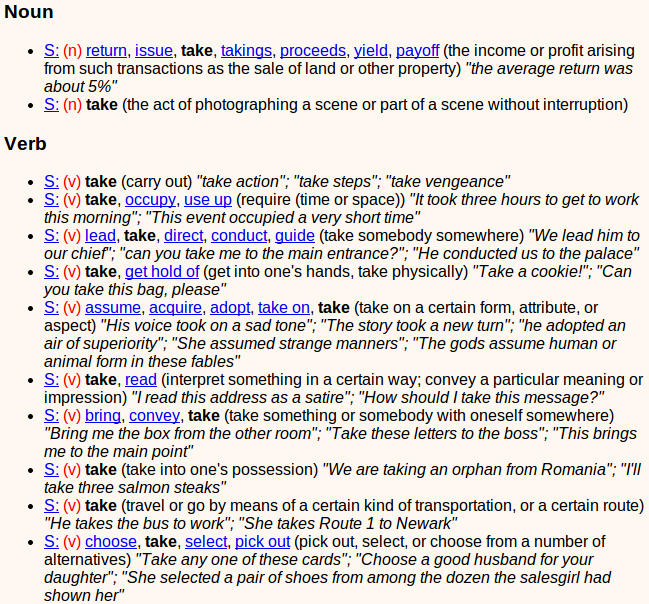
\includegraphics[width=12cm]{take-wordnet-31.png}
  \caption{Some of the WordNet 3.1 senses for ``take": there are two noun
  senses and 42 distinct verb senses, though we only show the first ten. In
  WordNet and similar projects, word senses are called \emph{synsets}, as there
  will be a set of synonyms that share the sense.}
  \label{fig:wordnet-senses-take}
\end{figure}

Treating WSD as a supervised learning problem requires labeled training data,
which for this task means text where each token has been annotated with its
appropriate sense identifier. 
Such corpora must be created manually specifically for this purpose, and this kind
of annotation is very labor-intensive, especially when annotating data for an
all-words WSD task, as the annotators must consider the many possible senses
for each word, and new words will occur during the course of annotation.

Sense-annotated corpora have been created for supervised WSD for both the
lexical selection and all-words settings, but they are only available for a few
languages, due to the time and effort required to prepare them.  Some famous
sense-annotated corpora include the ``hard/line/serve" corpus, originally
prepared by Leacock \emph{et al.}
\cite{Leacock:1993:CSS:1075671.1075730,leacock1998using}, which
marks occurrences of the adjective ``hard", noun ``line" and verb ``serve" with
their respective senses from WordNet.\footnote{Available at
\url{http://www.d.umn.edu/~tpederse/data.html}}
These feature roughly four thousand annotated instances of each word. Larger
lexical selection data sets were prepared for the first three SensEval shared
tasks\footnote{Archived at the same URL} (\cite{Kilgarriff98senseval}, XXX what
about 2 and 3?),
each of which featured 12 to 20 thousand labeled instances of 35 to 73
different word types.

There have also been all-words annotated corpora, such as the MASC and
SemCor corpora, which included XXX sentences annotated with their WordNet
senses... (XXX cite these too), and larger corpora produced with semi-automated
methods and manually verified.

In order to ameliorate this WSD data acquisition bottleneck and allow WSD
research to move forward in the absence of annotated training data, researchers
have also created corpora with artificially-ambiguous ``pseudo-words".  The
original uses are then considered two senses of the new pseudo-word, and
researchers can check whether their WSD algorithms can recover the original
token.

For a broad overview of the history of and different approaches to word sense
disambiguation, please see Agirre \emph{et al.}'s book on the topic.
\cite{agirre2006word}
Supervised-learning approaches are by no means the only strand of research;
there are also unsupervised word-sense induction approaches,
knowledge-based heuristics that make use of hand-crafted resources such as
dictionaries...
%% XXX

It has long been held that word sense disambiguation is a central problem in
NLP applications, including machine translation.
Even in popular culture, the dangers of misunderstanding and thus
mistranslating individual words is well-understood; many have heard the
(apparently apocryphal \cite{hutchins:whiskey}) story about an early MT system
faced with the Biblical saying ``the spirit is willing but the flesh is
weak" in Russian and producing (variations on the story abound) ``the vodka is
good but the meat is rotten".
Warren Weaver described, in his prescient 1949 memorandum \cite{weavermemo},
both an essentially modern conception of WSD and why a translation system would
need it.

As early as 1960, Yehoshua Bar-Hillel wrote that general-purpose machine
translation (``fully automatic high-quality  translation", as it was  called at
the  time) was impossible due to the insurmountable task of writing WSD
routines for all source-language words. \cite{barhillel1960}

\begin{quote}
During the past year I have repeatedly tried to point out the illusory
character of the FAHQT ideal even in respect to the mechanical determination of
the syntactical structure of a given source-language sentence... Here I shall
show that there exist extremely simple sentences in English -- and the same
holds, I am sure, for any other natural language -- which within certain
linguistic contexts, would be uniquely (up to plain synonymy) and unambiguously
translated into any other language by anyone with a sufficient knowledge of the
two languages involved, though I know of no program that would enable a machine
to come up with this unique rendering unless by a completely arbitrary and
\emph{ad hoc} procedure whose futility would show itself in the next example.

A sentence of this kind is the following: \emph{The box was in the pen.}
\end{quote}

To produce a correct rendering of this sentence in Spanish, for example, the
translation system must decide between translating ``pen" as \emph{corral} (an
enclosure, like for an animal) or as \emph{pluma} (the instrument for writing).

As of this writing, for this particular example, Google Translate picks the
correct rendering, although in September 2013, it chose the less-sensible 
``in the writing implement" translation (see Figure \ref{fig:box-in-pen}).

One wonders how this could have come about -- we would hope that the n-gram
language model for Spanish would prefer sentences about things in enclosures to
things in writing implements.
But the word \emph{en} can be a translation of either the English ``in" or
``on", and \emph{pluma} can also mean ``feather", so \emph{en la pluma} will be
attested in a large corpus of Spanish; we could easily imagine a sentence
containing ``on the feather". This situation is fairly complex.

\begin{figure}
  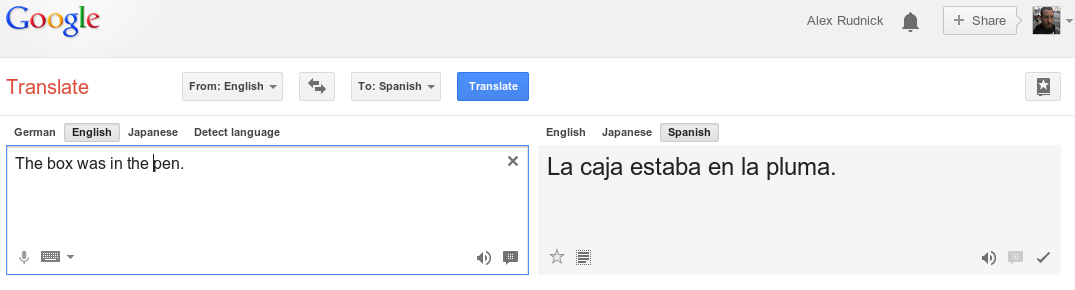
\includegraphics[width=12cm]{box-in-pen.png}
  \caption{Google Translate, September 17, 2013; interestingly, adding or
  removing the final period in the English sentence caused a switch between the
  ``pluma" and ``corral" renderings.}
  \label{fig:box-in-pen}
\end{figure}

In a translation task, even if we are able to assign a particular sense to a
given word, we must still map these senses to translations in the target
language, and there is no guarantee that senses identified by source-language
lexicographers will map neatly to distinctions made by the target language.

\section{Cross-lingual word sense disambiguation}
\label{sec:clwsd}

This problem that Bar-Hillel identified as difficult, the one that arises
in the apocryphal ``spirit is willing" story, is a particular variant of word
sense disambiguation that we here call \emph{cross-lingual WSD} (CL-WSD).
In a CL-WSD task, we  want to label words or phrases in the input text with
their contextually-appropriate translations in some target language. In this
case the
sense inventory for each word is defined as its possible translations.
Typically, the possible translations are discovered automatically from a
word-aligned bitext corpus, although a dictionary or other bilingual lexicon
may also be used as source of possible translations.

This setting for WSD has an immediate application in machine translation, and
in this case, it
also neatly addresses the problem of choosing an appropriate sense inventory,
which has historically been a difficult problem for the practical application
of WSD systems \cite{agirre2006word}. The sense distinctions that the system
should learn are exactly those that are lexicalized in the target language.
CL-WSD also sidesteps the ``knowledge acquisition bottleneck" hampering other
work in WSD \cite{lefever-hoste-decock:2011:ACL-HLT2011}.
While supervised CL-WSD methods typically require bitext for training, this is
more readily available than the sense-annotated text that would otherwise be
required; Gale \emph{et al.} suggested the use of sentence-aligned bitexts for
WSD research as early as 1992 \cite{gale1992method}.

WSD applied directly to machine translation has a long history; practical work
in integrating WSD with statistical machine translation particularly dates back
to early SMT work at IBM \cite{Brown91word-sensedisambiguation}.
Despite all of the ambiguities in translation,
most statistical MT systems do not use an explicit WSD module
\cite[Chapter~3]{agirre2006word};
the language model and phrase tables of these systems mitigate lexical
ambiguities by encouraging words used collocationally to appear together in the
output. Entire phrases\footnote{Not necessarily ``phrases" in a syntactic
sense, but subsequences of sentences} such as verbs with their common objects
may be learned and stored in the phrase table, and the language model will
encourage common collocations as well. CL-WSD techniques have been successfully
used to improve SMT, especially when it is applied not just to individual
tokens but to phrases present in the phrase table, as in the work of Carpuat
and Wu \cite{carpuatpsd}; there have also been discriminative classifiers used
to aid in selecting phrase table entries, as in the work of XXX (somebody from
Charles University or something? ...), which is equivalent, even if not
described by the authors in terms of word-sense disambiguation.

This cross-lingual variant of WSD has received enough attention to warrant
shared tasks at recent SemEval workshops: SemEval 2010 Task 3
\cite{lefever-hoste:2010:SemEval} and SemEval 2013 Task 10 \cite{task10} were
both classical cross-lingual lexical sample tasks. 
A similar task was also run in 2014 \cite{vangompel-EtAl:2014:SemEval},
although this task provides a target-language context rather than a
source-language one, more closely representing the problem faced by an agent
trying to help a second-language learner compose a sentence in their L2 than
that faced by a machine translation system.
Some approaches to the first two tasks, along with a number of other projects,
are described in Chapter~\ref{chap:relatedwork}.

In general, there is a many-to-many relationship across language boundaries
between words and their possible translations.
This happens for a number of reasons: figurative or metaphorical uses may not
translate directly,
obligatory information in one language may be left unspecified in another,
or the criteria for selecting a word may simply differ.
To give some familiar examples, a ``leg" of a trip in English is typically
translated as \emph{etape} in French, which is unrelated to limbs used for
walking (see Figure \ref{fig:leg} for a fuller view of the situation's
complexity);
translating ``brother" to Japanese requires specifying whether the brother is
older (\emph{ani}) or younger (\emph{ot\=oto});
a soap bubble or a ceramic plate can be destroyed with the same word in
Chinese, whereas English speakers distinguish between the verbs
``pop" and ``break" \cite{majid2007semantic}.

To take a look at some apparently easier examples, let us also consider the
following usages of \emph{letter}, from the test set of a recent SemEval shared
task \cite{task10}, and how to translate them into Spanish.

\enumsentence{
But a quick look at today's \emph{letters} to the editor in the Times suggest
that here at least is one department of the paper that could use a little more
fact-checking. }
\label{sent:carta}
\enumsentence{
All over the ice were little Cohens, little Levys, their names sewed in block
\emph{letters} on the backs of their jerseys. }
\label{sent:letra}

We would want (\ref{sent:carta}) to be translated with the word \emph{carta},
and (\ref{sent:letra}) to be translated with \emph{letra} or something similar.
Google Translate (as of this writing) handles both of these sentences well,
rendering the first with ``cartas" and the second with an even better choice,
translating the phrase ``block letters" as \emph{mayúsculas}.
However longer-distance relationships, search errors, or simple statistical
accidents can still cause strange translations in practice.

\begin{figure}
  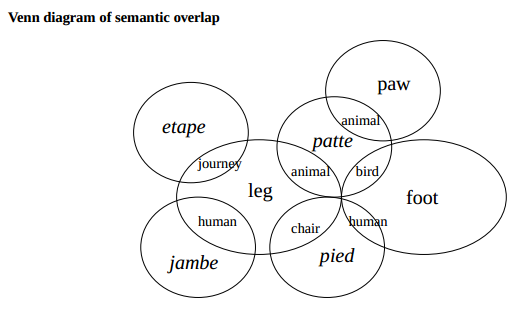
\includegraphics[width=12cm]{hutchins-leg-etc.png}
  \caption{Overlap of words related to ``leg"; relationships between English
  and French words. Figure 21.2 from \protect\cite{slp1}; example originally
  from \protect\cite[Chapter 6]{hutchins1992introduction}.}
  \label{fig:leg}
\end{figure}

\section{Hybrid MT}
Recently there has been renewed interest in machine translation systems that
take into account syntactic structure, linguistic knowledge, and semantic
representations, perhaps due to a perception that statistical approaches
relying on flatter phrase-based representations and hierarchical
representations not based on linguistic intuitions are reaching a performance
plateau.

%% XXX: could use some citations.
The boundaries between rule-based and statistical MT systems are becoming
increasingly blurred, and hybrid systems are being developed in both
directions, with RBMT systems incorporating components based on machine
learning, as well as SMT systems making use of linguistic knowledge for
morphology and syntax.
Rule-based components are especially applicable in cases where the language
pair involves predictable reordering through syntactic divergences
(XXX citation)
and in cases where one or both sides of the translation pair exhibits rich
morphology; morphological analysis and generation software generally consists
of hand-written rules in the form of finite-state transducers.

Additionally, for most of the world's language pairs, there is simply no large
bitext corpus available, so training a purely statistical machine translation
system is infeasible.\footnote{Techniques for learning from comparable corpora,
such as translation spotting, are under development, and there has been some
work on building sufficiently large bitext corpora through crowdsourcing, but
these approaches have not yet reached wide adoption.}
As such, RBMT approaches are still relevant for many language pairs, and there
is a vibrant research community focused on building linguistically-informed
primarily rule-based machine translation systems.

We would like for RBMT or hybrid systems, once developed, to be able to make
use of any bitext resources that are available, or that become available later.
Like SMT systems, they should be able to produce better translations as larger
corpora are developed, without additional code changes: this is the main
engineering goal for the Chipa software.

\urldef{\leydelenguas}\url{http://www.cultura.gov.py/lang/es-es/2011/05/ley-de-lenguas-n%C2%BA-4251/}

\section{Paraguay and the Guarani Language}
Guarani is an indigenous language spoken in Paraguay and the surrounding
region.
It is the historical native language of the indigenous Guarani people. The
word for the Guarani language in Guarani is \emph{avañe'e} (``people's
language", where \emph{ñe'e} means ``language").

Guarani is unique among indigenous American languages in that a substantial
number of non-indigenous people speak it. The majority of Paraguayans are
conversant in Guarani, although they are likely to be bilingual with Spanish.
In practice, many Paraguayans use a combination of Guarani and Spanish called
\emph{Jopar{\'a}}, which is the Guarani word for ``mixture".

Paraguay is officially a bilingual, pluricultural country, as described by its
famous \emph{Ley de Lenguas} \footnote{\leydelenguas} (``Law of Languages").
However, the Guarani language is at a significant social and economic
disadvantage and is typically not used in formal situations, as Spanish is
considered more prestigious. There are, however, an engaged activist
community, many Guarani-language educators, and a government agency devoted
specifically to policy regarding language.
The Guarani language figures significantly into a sense of Paraguayan national
identity and history.

Guarani has a rich, polysynthetic, agglutinative morphology, in which roots can
derive into different parts of speech, and often several roots can combine into
a single word. Guarani morphology can mark tense, aspect (even on nouns),
number, negation, and other features. However, unlike Spanish, it has no
grammatical gender.  Guarani's rich morphology can make many NLP tasks,
including ones seemingly as simple as spell-checking, rather challenging.

We are in contact with a number of collaborators in Paraguay, including
language activists and educators from the \emph{Ateneo de la Lengua y Cultura
Guaraní} \footnote{\url{http://www.ateneoguarani.edu.py/}} and the
\emph{Fundación Yvy Marãe'{\~y}} \footnote{\url{http://yvymaraey.org/}},
both of which are schools that offer training for Guarani-language translators.
We have also been discussing plans with several local software
developers, including members of the local One Laptop Per Child organization
and the Secretariat of Language Policies. Our crowdsourcing and
collaborative translation system \cite{RUDNICK14.151} is currently under
development with feedback from professors from the \emph{Ateneo} and
policymakers at the Secretariat.

\subsection{Online Language Tools for Guarani}
There are currently very few online language tools for Guarani; some of the
best available ones are iGuarani \footnote{\url{http://iguarani.com/}}, a
searchable online dictionary and gisting translation system developed by young
Paraguayan programmer Diego Alejandro Gavilán.

There is also a small searchable online dictionary developed by Wolf Lustig
\footnote{\url{http://www.uni-mainz.de/cgi-bin/guarani2/dictionary.pl}},
which has versions in Spanish, German, and English. He has graciously made this
dictionary available for our use, and this will provide a starting point for
our Spanish-Guarani translation system.

The Guarani activist and education community has a presence on the Web,
although a startlingly large fraction of this presence is a single author,
David Galeano Olivera, the president of the \emph{Ateneo}.
He has collected a number of resources, written in Spanish
and Guarani, about the Guarani language and the culture surrounding it.
\footnote{\url{http://cafehistoria.ning.com/profiles/blogs/la-lengua-guarani-o-avanee-en}}

\chapter{Data Sets, Tasks, Software and Evaluation}
\label{chap:evaluation}
In order to evaluate our CL-WSD approaches and their effects on translation
quality, we will need to have a basis for comparison between our proposed
techniques and sensible baselines, including results reported by other
researchers.

In this chapter, I describe the tasks and data sets that we will investigate
for the rest of the dissertation, as well as the basic version of the Chipa
software, which we extend in a variety of directions in the following chapters.

As discussed in Section \ref{sec:background-wsd}, for many years word sense
disambiguation systems have been evaluated \emph{in vitro} and in a monolingual
setting. The test sets for such WSD evaluations include sentences
hand-annotated with a word senses from a particular sense inventory, such as,
typically, the WordNet senses. These monolingual WSD evaluations often include
both coarse-grained and fine-grained distinctions and allow for several
possible correct answers; some word senses identified by lexicographers are
more closely related than others.  While the senses in a sense inventory will
contain many useful and interesting distinctions, they do not necessarily make
the distinctions most appropriate for a given task, wich will vary by
application. As such, accuracy improvements on these tasks do not necessarily
lead to performance gains for an NLP system making use of word-sense
disambiguations \cite{resnikwsdapplications}.

This style of evaluation relies on a fairly scarce resource: sentences
hand-annotated with a particular sense inventory.
In the CL-WSD setting, where we consider target-language lexical items to be
the salient senses of source-language words, we could also ask annotators to
hand-label each word of our test sentences with their translations.
For many language pairs, however, this annotation task has nearly been
performed by translators. We do not strictly have the labels for each token in
the source document, but with automatic word alignment techniques, we can infer
these labels with high confidence.

\section{Measuring MT Improvements}
We will additionally want to conduct \emph{in vivo} evaluations of our CL-WSD
techniques as applied to running MT systems. Here we can use standard
approaches for evaluating MT, such as BLEU and METEOR scores, or simply show
that where word choices differ with the application of CL-WSD, the changes are
for the most part improvements. For these experiments, we sample sentences
from the available bitext -- particularly sentences that contain polysemous
words for which we can train classifiers -- and run the MT systems both with
and without Chipa enabled.

We want to make the argument that improved classification accuracy on CL-WSD
tasks leads to improved translation results.
But in general, the addition of CL-WSD has not been an overwhelming success in
statistical machine translation, especially when we have large corpora
available for language modeling \cite{carpuatpsd}.
It seems intuitive that a
classifier producing correct word choices would lead an MT system to produce
better results. But we do not have a system that always indicates correct word
choices, nor are we likely to have one in the near future. And it is an
empirical question, whether the suggestions made by the CL-WSD system,
imperfect as they are sure to be, will improve translation results. We could
imagine gains failing to materialize, for example, if the CL-WSD system's
correct choices are mostly those that the MT system would have made on its own,
say with the guidance of a language model and phrase-table probabilities. 
We could even imagine its incorrect choices being misleading to the point of
doing harm to our translation quality.

These experiments are described in more detail in
Chapter~\ref{chap:integration}, where I also discuss how to integrate Chipa
into the different machine translation packages.

\section{Measuring CL-WSD Classification Accuracy}
One straightforward \emph{in vitro} approach for evaluating a CL-WSD system is
to measure classification accuracy over pre-labeled data. Here by
classification accuracy, we mean measuring how often the system is able to
correctly choose an appropriate translation for the focus word in a given
context.
Strictly speaking, we
do not have pre-labeled data: our bitext does not come with sub-sentential
alignments. But automatic word alignments provide a good approximation, as long
as our sentence alignments (or verse alignments, for Bible text) are accurate.
For the purposes of this work, we will assume that the automatic word-level
alignments are correct, putting in our best effort at preprocessing the
available text so that the aligner can produce useful output.

Using our automatically-aligned bitext as labeled data allows us to closely
mirror the lexical selection task faced by an MT system while translating
running text. We can train classifiers for many different word types, but we
will generally not have training examples available for all words in the input
at test time. This is a problem faced by data-driven NLP systems broadly.

For comparison with other work, in Section \ref{sec:baseline-semeval} we run
our systems on the SemEval CL-WSD shared task test sets, which are publicly
available.  Our larger task here is framed in the same way as the CL-WSD shared
tasks from 2010 and 2013, so measuring performance on these test sets allows a
straightforward comparison between the variations explored in this work and
several other CL-WSD systems from recent years. These test sets are limited in
scope, however, and will only demonstrate Chipa's performance for translating
individual English nouns. It is also worth noting that our more immediate
practical goal is to aid translation from Spanish into lower-resourced
languages. 

\section{Data Sets and Preprocessing}
The largest corpus that we have available for all of our source and target
languages is the Bible. There are translations available for many different
languages, and while these were not always produced by native speakers, the
translators are often driven by missionary zeal to produce high-quality
translations~\cite{DBLP:journals/lre/ResnikOD99}, so we can be reasonably
confident of the (linguistic) accuracy of our text.

In this work, we focus on one Bible translation per language. For Spanish, we
use the Reina-Valera translation (1995 edition), which I was able to scrape
from a Bible study website. Our Guarani translation, \emph{Ñandejara Ñe'e}
(1997 edition) was scraped from the same site. Our Quechua version (the 2004
translation published by the Peruvian Bible Society) was provided by Chris Loza
and Rada Mihalcea; the preparation of the Quechua corpus is described in Loza's
masters thesis \cite{chrisloza}. For English, we use the public domain World
English Bible translation.
While there are a large number of translations available online, different
``Bible societies" often own the associated copyrights and thus redistribution
of the complete texts is often restricted \cite{MAYER14.220.L14-1215}.

\subsection{Source-side annotations}
\label{sec:annotations}
In order to gracefully include a variety of features and build on
any available analysis tools for the source language, Chipa's input format and
feature functions allow for arbitrary annotations on source-language tokens.

Chipa's input file format describes one token per line, with fields split by
tabs.  The first field of a line is a token's lemma, and the second field is
its surface form. Following this are an arbitrary number of annotations for
that token, which may encode information such as part-of-speech, dependency
relations, or similar.  Sentence boundaries are indicated by blank lines. An
annotated sentence with one annotation per token might look like Figure
\ref{fig:quickbrownfox}, for example:

\begin{figure*}
\raggedright \texttt{\\
the	The	pos=DET \\
quick	quick	pos=ADJ \\
brown	brown	pos=ADJ \\
fox	fox	pos=NOUN \\
jump	jumped	pos=VERB \\
over	over	POS=ADP \\
the	the	POS=DET \\
lazy	lazy	POS=ADJ \\
sleep sleeping	POS=VERB \\
dog	dog	POS=NOUN \\
.	.	POS=. \\
  }
  \caption{Example annotated sentence.}
  \label{fig:quickbrownfox}
\end{figure*}

The Chipa software has been developed with a number of tools that consume and
produce this format, typically taking in sentences annotated in this way,
calling another NLP tool to generate more annotations, and then adding the new
annotations to those already present. The experiments in this chapter only use
one of these tools, \texttt{freeling\_to\_annotated.py}, which produces Chipa's
input format given output from Freeling.  In the following chapters, we will
make use of these tools and the extra information they make available to our
classifiers; in Chapter \ref{chap:monolingual} we add annotations learnable
with monolingual resources, and in Chapter \ref{chap:multilingual} we describe
tools and annotations that require parallel data.

\subsection{Preprocessing}
There is a nontrivial amount of preprocessing required in order to get our
Bible text into a format suitable for our tools.  This is largely due to the
varying markup formats used by different translation publishers.
For each of the available translations, we need to understand its formatting
enough to know which text comes from which book, chapter, and verse number.
This triple uniquely identifies a unit of text, and verse numbers are nearly
standardized across translations.  There are a few exceptions, however:
translations produced by different religious traditions may include different
books. Most notably, Catholic editions have a superset of the books found in
modern Protestant editions, and include slightly different chapters.
Additionally, in some translations, such as our Guarani edition, a few verses
have been combined into a single segment for a more natural translation.

In any case, if a particular book/chapter/verse is present in two Bibles, then
the two verses are very likely translations of one another. Once we find all of
the matching verses, we can build a bitext corpus suitable for use in our
pipeline.  In all four of our translations, we find all 66 books of the
Protestant Bible. Furthermore, we find matches for nearly all of the verses
across all of the language pairs considered. For English/Spanish and
Spanish/Quechua, the intersection of book/chapter/verse tuples across Bibles
contains over 99\% of the verses in any given Bible. For the Guarani
translation, however, we are only able to match 95.2\% of the verses. The
Guarani text contains fewer verses, $29,867$ versus the $31,104$ in Spanish,
showing that the translators were more willing here to combine verses and that
the translations may be more interpretive.

Our English translation is distributed in a format called USFM (Unified
Standard Format Markers), which is a markup language developed by a working
group of Bible translators and used widely by the Bible-related software
community; see Figure \ref{fig:usfmsample} for some sample input text in this
format.
\footnote{See \url{http://paratext.org/about/usfm} for more about USFM. USFM is
widely deployed; the website from which we scraped the Spanish and Guarani
corpora appears to render its HTML from a USFM source.  There is an entire
community of Bible software developers, and it has a wing that advocates Open
Source software and translations unencumbered by copyright.  One could delve
arbitrarily deeply into the history of religious-text translators and their
relationships with technology and copyright, but one has an NLP dissertation to
write.}
While there are a number of tools that consume USFM, I did not find one that
handles our particular use case of stripping metadata and simply mapping from
verses to flat text, so I wrote a short script, \texttt{parse\_usfm.py}, to
parse USFM and produce text in an easily-alignable format.

Our Spanish and Guarani corpora are extracted from HTML pages scraped from an
online Bible study website. In practice, the scraping was done by predicting
the URLs for each chapter of each book and requesting those URLs
programmatically. We then extract the text from the saved HTML pages with a
Python script and the BeautifulSoup library for HTML parsing.
\footnote{\url{http://www.crummy.com/software/BeautifulSoup/}}
As a side note, since websites change over time and we
downloaded the Guarani translation at an earlier date (from a mobile version of
the site that is no longer available), the HTML takes a significantly different
structure in the Spanish and Guarani editions, so they require different
versions of the script for preprocessing; see Figures \ref{fig:es-html-sample}
and \ref{fig:gn-html-sample} respectively for representative Spanish and
Guarani input.

Our Quechua translation came in an easily parseable format, with individual
verses already identified by Loza and Mihalcea; for this corpus, relatively
little preprocessing was necessary since lines begin with the book, chapter,
and verse already labeled. See Figure \ref{fig:loza} for a sample of the input
format.
It is conceivable that there are inconsistencies introduced by the
text-extraction processes for these different data sources, but for the most
part the scripts seem reliable, since they result in approximately the same
number of verses and tokens for our different languages, and the great majority
of the sentences are alignable (see subsequent discussion on bitext alignment).
Additionally, hand inspection of the text for the languages that I can
personally read (English and Spanish) show that the text contains fairly close
translations, and loan words and similar named entities appear in the Quechua
and Guarani texts.

\begin{figure*}
\raggedright \begin{verbatim}
\id LAM 25-LAM-web.sfm World English Bible (WEB) 
\ide UTF-8
\h Lamentations 
\toc1 The Lamentations of Jeremiah 
\toc2 Lamentations 
\toc3 Lam 
\mt2 The 
\mt Lamentations 
\mt2 of Jeremiah 
\c 1  
\p
\v 1 How the city sits solitary, 
\q2 that was full of people! 
\q She has become as a widow, 
\q2 who was great among the nations! 
\q She who was a princess among the provinces 
\q2 has become a slave! 
\b
\q
\v 2 She weeps bitterly in the night. 
\q2 Her tears are on her cheeks. 
\q Among all her lovers 
\q2 she has no one to comfort her. 
\q All her friends have dealt treacherously with her. 
\q2 They have become her enemies. 
\end{verbatim}
  \caption{The first two verses of the Book of Lamentations (World English
  Bible translation) in USFM format.}
  \label{fig:usfmsample}
\end{figure*}

\begin{figure*}
\raggedright \begin{verbatim}
[999,31,1,1] ¡Ay, imaraqmi Jerusalenqa sapan kapushan, haqay hina
  askha runakunayoq llaqta! ¡Ay, imaraqmi viuda warmi hina kapushan,
  lliw suyukunaq uman kashaqqa! Mit'anipina llank'apushan, lliw
  llaqtakunaq ñust'an kashaqqa.
[999,31,1,2] Tutan-tutanmi unuy-parata waqayku- shan, uyapas
  p'aspay-p'aspallaña. Llapan munaqninkunamanta manan hukllapas kanchu
  sonqochay- kuqnin. Llapan reqsinakuq-masinkunapas manan rikuqpas
  tukupunkuchu, llapallanmi awqanman tukupunku.
\end{verbatim}
  \caption{The first two verses of the Book of Lamentations in Quechua, from
  the 2004 Peruvian Bible Society translation. Whitespace changes added here
  for readability.}
  \label{fig:loza}
\end{figure*}

\begin{figure*}
\raggedright \begin{verbatim}
<div id="reader" class="content text_ltr">
  <a name="1"></a>
  <a href="/bible/more/Lam.1.1"
     style="color:black;text-decoration:none">
    <h2>El profeta </h2>
    <span class="verse" id="Lam_1_1">
    <strong class="verseno">1</strong>
    &nbsp;¡Pobrecita de ti, Jerusalén! <br />
    Antes eras la más famosa <br />
    de todas las ciudades. <br />
    ¡Antes estabas llena de gente, <br />
    pero te has quedado muy sola, <br />
    te has quedado viuda!  <br />
    ¡Fuiste la reina de las naciones, <br />
    pero hoy eres esclava de ellas! <br /> <p> </p></span>
  </a>
  <a name="2"></a>
  <a href="/bible/more/Lam.1.2"
     style="color:black;text-decoration:none">
    <span class="verse" id="Lam_1_2">
  <strong class="verseno">2</strong>
    &nbsp;Olvidada y bañada en lágrimas <br />
    pasas todas las noches. <br />
    Muchos decían que te amaban, <br />
    pero hoy nadie te consuela. <br />
    Los que se decían tus amigos <br />
    hoy son tus enemigos. <br />
    <p> </p></span>            </a>
\end{verbatim}
  \caption{The first two verses of the Book of Lamentations, \emph{Traducción en
  Lenguaje Actual} (TLA) version, in HTML as scraped from the web. Whitespace
  changes added here for readability.}
  \label{fig:es-html-sample}
\end{figure*}

\begin{figure*}
\raggedright \begin{verbatim}
<div class="ltr" data-abbreviation="gdc" data-reference="lam.1.gdc"
     data-usfm="LAM.1" id="version_primary">
    <div class="version vid66 iso6393nhd" data-vid="66"
         data-iso6393="nhd">
        <div class="book bkLAM">
            <div class="chapter ch1" data-usfm="LAM.1">
                <div class="label">1</div>
                <div class="s">
                    <span class="heading">Ñembyasy Jerusalén oñehundi
                    haguére</span>
                </div>
                <div class="q1">
                    <span class="content" />
                    <span class="verse v1" data-usfm="LAM.1.1">
                        <span class="label">1</span>
                        <span class="content">Ajépa ha'eño
                        ajejuhu</span>
                    </span>
                </div>
                <div class="q1">
                    <span class="verse v1" data-usfm="LAM.1.1">
                        <span class="content">upe táva
                        guasuete,</span>
                    </span>
                </div>
    ...
\end{verbatim}
  \caption{The beginning of the Book of Lamentations in Guarani,
  \emph{Ñandejara Ñe'e} version, in HTML as scraped from the web. Whitespace
  changes added here for readability. Note the metadata included here,
  suggesting that the HTML is generated programmatically from an underlying
  USFM document.}
  \label{fig:gn-html-sample}
\end{figure*}

Each of the different formatting schemes uses its own encoding to identify the
different books of the Bible, so when producing output for alignment, we must
map to a standard encoding. For example, our Quechua edition marks the book of
Lamentations with the numerical code $31$ (it is the thirty-first book in
modern Catholic editions), but in the USFM markup for the English translation,
we find a header with the string ``Lamentations". For our Spanish and Quechua
editions from the web, we find the code ``LAM" in the markup. In any case, we
map each of these identifiers to a single code ``Lam", so that we can match
books, chapters and verses across translations.

\subsection{Morphological Analysis}
\label{sec:guaranima}

For each of our languages, whether on the source or target side, in addition to
tokenizing, lowercasing and verse-alignment, we extract the lemmas (the
citation forms, normalized with respect to inflection) from each surface word.
Especially when working with smaller data sets and morphologically rich
languages, this is an important step; working primarily with lemmas rather than
surface-form words allows us to group, for example, the plural form of a word
with its singular.

For English and Spanish, we use the FreeLing suite of NLP tools
\cite{padro12} to extract lemmas. FreeLing provides a variety of analyses,
including tokenization, sentence splitting, multi-word expression and named
entity detection, part-of-speech tagging and parsing.  We start out using just
a few of these tools -- initially only tokenization and lemmatization. We
discuss making use of more of them in Chapter \ref{chap:monolingual},
leveraging the quality NLP tools that we have for our resource-rich source
languages.

The use of FreeLing for English is a noted improvement over initial
experiments, which used the WordNet lemmatizer and the default NLTK
part-of-speech tagger; these tools do not, as distributed, support Spanish.
The WordNet lemmatizer has a fairly small vocabulary, did not
provide a good strategy for dealing with unknown words, and could only address
nouns, verbs, and adjectives.
There are a very large number of named entities in the source text, most of
which are not present in WordNet. It cannot, by itself, help us know that
``Zebulonites" is the plural of "Zebulonite".  37\% of the tokens in our
English translation of the Bible are not present in WordNet, and many of these
tokens are function words. However, there are quite a few named entities in the
Bible: 33\% of the word types are not covered by WordNet either.

For Guarani and Quechua, we use Michael Gasser's ParaMorfo and AntiMorfo
analyzers.\footnote{Prof. Gasser's morphology software for Guarani, Quechua,
Spanish, and other languages is available at
\url{http://www.cs.indiana.edu/~gasser/Research/software.html}} Guarani text is
analyzed with ParaMorfo 1.1, and Quechua with AntiMorfo 1.2.  These packages
are based on software originally developed for Ethiopian Semitic languages
\cite{gasser:eacl09}, and use cascades of finite-state transducers (FSTs),
which is a common approach in morphological analysis \cite{beesley+karttunen}.
ParaMorfo and AntiMorfo use weighted FSTs to handle long-distance dependencies
between morphemes, but rather than having weights correspond to probabilities
to be combined with multiplication, the FSTs are weighted with feature
structures that are combined via unification. This approach was originally
introduced by Amtrup \cite{amtrup:03}. In an FST weighted with feature
structures, the result of a successful traversal is the unification of the
feature structure ``weights'' on the traversed arcs, as well as an output
string. All possible paths through the FST are searched, though many of these
paths will not lead to accepting states, or will fail due to unification
conflicts.  Because a feature structure is accumulated during the process of
transduction, each traversal through the transducer retains a memory of where
it has been, permitting the incorporation of long-distance constraints such as
those relating the negative prefix and suffix of Guarani verbs.

Here the result of morphological analysis of a word is a root and a feature
structure representing the grammatical features of the word.  For the basic
version of Chipa, we are only concerned with the lemmatized forms of the words
in our corpora, so we ignore the grammatical features for now.  In cases of
morphological ambiguity, which is to say cases where a surface form could be an
inflection of multiple distinct lemmas, we maintain this ambiguity rather than
trying to disambiguate from context.  The different possible lemmas are
separated by a slash; there are examples of this in
Figure ~\ref{fig:gn-qu-morpho-ambiguity}.

\begin{figure*}
\begin{itemize}
  \item Quechua: \emph{Llapan munaqninkunamanta manan hukllapas kanchu
  sonqochay- kuqnin.} is analyzed by AntiMorfo as \texttt{llapan
  munaqninkunamanta ma/mana huk/huklla ka/kanchu sonqochay - kuqnin}.
  \emph{manan} here could be an inflection of \emph{ma} 'certainly' or
  \emph{mana} 'no, none'. Similarly with \emph{huk} 'one, another one' /
  \emph{huklla} 'only, lonesome, single' and \emph{ka} 'yours' /
  \emph{kanchu} (a kind of bird).
  \item Guarani: \emph{Upe che ro'o ha upe che pire ombyaipa, umi che kãngue
  omopẽmba.} is analyzed by ParaMorfo as \texttt{upe
  che so'o ha upe che pire ombyaipa , umi che kã mopẽ/pẽ . }. Here
  \emph{omopẽmba} is ambiguous, and could be an inflection of \emph{mopẽ} 'to
  break (something)' or \emph{pẽ} 'to break (oneself)'.
\end{itemize}
\caption{Examples of morphological ambiguity in Quechua and Guarani,
having been run through AntiMorfo and ParaMorfo. The Quechua text is the first
sentence of Lamentations 1:2; the Guarani is Lamentations 3:4.}
\label{fig:gn-qu-morpho-ambiguity}
\end{figure*}

%% TODO "Did you run / are you planning to run another experiment where you
%force disambiguation? Either use the highest weights, or the first analysis
%..."
%% Force morphological disambiguation on the gn side, not a bad idea.

There are, of course, examples of morphological ambiguity in English and
Spanish. A familiar example from Spanish is that \emph{ir} 'to
go' and \emph{ser} 'to be' sharing their preterite-tense forms; this is a
fairly common phenomenon. However, the FreeLing analysis tools can typically
(heuristically) resolve these ambiguities for us, and in this work we assume
that the Freeling output is correct, or at least correct enough.

\subsection{Alignment}
As a precaution against verses that are not close translations, or perhaps have
combined several parts of the text together into one verse on only one side, we
run the cdec filtering tool (\texttt{filter-length.pl}) with its default
settings, which checks for unusual length disparities in the bitext. This ends
up removing roughly 7\% of the verses\footnote{Specifically, length filtering
removes $7.12\%$ of the verse pairs for Spanish-English and thus
English-Spanish, $6.69\%$ for Spanish-Guarani, and $6.72\%$ for
Spanish-Quechua.}, but manual inspection shows that those verses removed are in
general very loose translations, or that additional material is present on one
side.

Having tokenized, lowercased, verse-aligned and lemmatized, our corpora, we are
ready to extract word-level alignments.
For this we use the \texttt{fast\_align} tool from cdec
\cite{dyer-EtAl:2010:Demos}, with its default settings\footnote{With the
command given at \url{http://www.cdec-decoder.org/guide/fast_align.html}} and
the lemmatized text as input.
\texttt{fast\_align} runs several iterations of a variant of IBM Models 1 and
2, with a prior encouraging diagonal alignments
\cite{dyer-chahuneau-smith:2013:NAACL-HLT}.
While running, it tunes the parameters on the priors, and having learned a
translation model, outputs the single most likely one-to-many word alignments,
such that each source language token is linked with zero or more
target-language tokens in the corresponding verse.

%% XXX: should explain the difference between what fast_align is doing and the
%% basic Models 1 & 2.
%% TODO "explain? example?"
%% XXX: working here

\TODO{add a clear example alignment here, maybe a word aligned to a multi-word
expression}

\subsection{A deeper dive: producing Spanish-Guarani bitext}
To get a concrete idea about the process of producing our bitext and our
annotated source corpus, we will now step through the bitext production process
for our Spanish-Guarani language pair. For the precise process, please see the
source code
\footnote{\url{https://github.com/alexrudnick/terere/tree/master/bibletools}}.

We consider the ``raw materials" for this process to be the scraped Spanish and
Guarani bibles; see Figure \ref{fig:es-html-sample} for an example.  In order
to replicate this work, or to extend it to more languages, one will have to
acquire bitext covering one's preferred language. There are translations in
many different languages available on various Bible websites, however.

The result of the scraping process is a directory full of HTML files, the raw
HTML that was served by the Bible websites. For the sites that we scraped, each
chapter is served as an individual HTML file. From these HTML files, we must
extract the flat text of all of the available Bible verses.  We do this with
the \texttt{get\_verses.py}, a tool that uses BeautifulSoup to parse the input
HTML and navigate its structure, extracting the verse identifiers and verse
text as it goes. We call the output of \texttt{get\_verses.py} a ``Bible file";
it consists of tab-separated values, one per line, in which (book, chapter,
verse) tuples are paired with the text of those verses.

We then call the \texttt{print\_bitext.py} on pairs of Bible files. This script
finds matching verses (book, chapter, verse tuples) and produces bitext files
in the format expected by the cdec alignment tools, which is simply
source-language segments and target-language segments, separated by
\texttt{|||}. The output of \texttt{print\_bitext.py} is called
\texttt{bible.es-gn.unfiltered}, which contains some non-parallel "sentences"
and is untokenized. Individual sentences have not been preprocessed at all.

We then a filtering script from cdec, \texttt{filter-length.pl}, which filters
out segments where either side is too long, or where there is a large disparity
in length between source and target text, which indicates input segments that
are not close translations. After this filtering step, we have selected the
bitext from which we will train Chipa. See Sentences \ref{sent:wood-en} and
\ref{sent:wood-es} for an example of a pair of segments that is filtered by
this step. This is 1 Kings 18:33, and the beginnings of these segments clearly
have the same meaning; for the Spanish translation, though, the material in the
second sentence of the English text has simply been moved into the subsequent
verse (1 Kings 18:34) for whatever reason.

\begin{figure}
\enumsentence{
He put the wood in order, and cut the bull in pieces, and laid it on the wood.
He said, “Fill four jars with water, and pour it on the burnt offering, and on
the wood.”}
\label{sent:wood-en}
\enumsentence{
 Preparó la leña, cortó el buey en pedazos, lo puso sobre la leña,
}
\label{sent:wood-es}
  \caption{Segments filtered due to length disparity. Our English and Spanish
  versions of 1 Kings 18:33.}
  \label{fig:length-disparity}
\end{figure}

Given the sentence-aligned bitext corpus, which contains only the subset of the
source and target Bibles that we were able to verse-align (roughly, ``sentence
align", in more common MT terms, though a verse need not be a single sentence),
we now want to preprocess the source text to produce the annotated version used
for training. We call cdec's \texttt{cut-corpus.pl} to select just the source
side of the bitext, in this case the Spanish. Then we call Freeling to do basic
analysis on the input Spanish text: it provides tokenizing (for example,
splitting out punctuation adjacent to words), lemmatizing and tagging
\footnote{See the checked-in Freeling configuration file for the exact settings
used:
\url{https://github.com/alexrudnick/terere/blob/master/bibletools/freeling-config/es.cfg}}.
Then we run a Python script, \texttt{freeling\_to\_annotated.py}, to convert
the FreeLing output format into Chipa's source-language input format.

Now on the target language side, we do something analogous, although less
analysis of the target text is required, and Freeling does not support our
target languages. We again use \texttt{cut-corpus.pl} to select just the target
side, in this case the Guarani, and cdec's \texttt{tokenize-anything.sh} and
\texttt{lowercase.pl} to tokenize and lowercase the Guarani text. Then we run
Chipa's lemmatizer script over the Guarani text. It calls the Paramorfo
morphological analyzer on the Guarani tokens, producing Guarani lemmas. In
cases of morphological ambiguity, we produce tokens that maintain that
ambiguity, simply joining the possible lemmas with a slash.  Once lemmatization
is complete, we have produced the target-language lemmatized text.

Then we join together each line of the source-language lemmatized text with its
corresponding target-language lemmatized text, using cdec's
\texttt{paste-files.pl} script. The output of this is the sentence-aligned,
tokenized, lowercased, lemmatized bitext corpus, which is ready for word
alignment. To generate the word alignments, we call cdec's \texttt{fast\_align}
tool.

\begin{figure*}
\begin{tikzpicture}[scale=0.7]
  \tikzstyle{vertex}=[rectangle,rounded corners, fill=gray!80!white,draw=gray!70!black,
  minimum size=0.6cm,line width=1]
  \draw[step=1cm,draw=gray] (0,0) grid (10,13);

  \foreach \y/\f in {0/Amargamente, 1/llora, 2/en, 3/la, 4/noche, 5/y, 6/las,
  7/lagrimas, 8/corren, 9/por, 10/sus, 11/mejillas, 12/.} {
    \node[left] at (-.2,12.5-\y) {{\raggedleft \f }};
  }
  \foreach \x/\e in {
  0/Pyhare, 1/pukukue, 2/hasẽ, 3/{,}, 4/ha, 5/hesay, 6/mante, 7/hováre,
  8/osyry, 9/. } {
    \node[rotate=60,right] at (\x+.4,13.2) {{\raggedright \e}};
  }

  % draw word alignment
  \foreach \y/\x in {
  4/0, 4/1, 1/2, 3/3, 5/4, 7/5, 9/6, 11/7, 8/8, 12/9
  } {
    \node[vertex] at (\x+.5, 12.5-\y) {};
  }
\end{tikzpicture}
  \caption{A sample word alignment. The beginning of Lamentations 1:2, mapping
  from Spanish to Guarani. Alignment produced with \texttt{fast\_align}.}
  \label{fig:example-word-alignment}
\end{figure*}

After all of this preprocessing and alignment, we have produced three files of
interest to Chipa: first, we have the lemmatized bitext corpus. Second, we have
the one-to-many word alignments between the two sides of the bitext. These two
files taken together constitute the ground truth for the Chipa system -- the
source lemmas, and the subsequences of the target text that are considered to
be their translations. Note that these alignments could be NULL -- a source
word could correspond with an empty subsequence of target-language tokens. At
test time, we will want to predict those translations, whatever they happen to
be.

The third file contains the annotated version of the source text, which
includes all of the information of the source side of the preprocessed bitext,
in addition to the original surface forms and the annotations extracted from
FreeLing analysis. Further annotations can be added by other tools; in general,
annotated source-language corpora could contain whatever kinds of signals we
might like to add to aid classifiers in predicting translations. In Chapter
\ref{chap:monolingual}, for example, we discuss features learnable with
monolingual resources such as part of speech tags, Brown clusters, and
embeddings learned with neural networks. In Chapter \ref{chap:multilingual}, we
discuss features that require parallel corpora, such as CL-WSD predictions into
languages other than the current target language. But in all of these cases,
the additional features are passed to the classifiers via this
corpus-annotation approach.


\section{Exploring the Bitext}
\label{sec:exploring}
Even using only the Bible as bitext, we find a substantial number of
training examples for many of the most common word types, which, due to the
Zipfian distribution of word types in most texts, constitute a significant
fraction of the tokens exhibited. See Figures \ref{fig:mostcommon-lemmas} and
\ref{fig:mostcommon-surface} for more detail.
%% TODO: quantify this, per language!!
Some of these most common words
in the text are proper names or exhibit only one translation in the target
language, but for the most part we see, through the aligned bitext, that
the most common words are polysemous.
To take a few salient examples from the Spanish-English aligned text,
the verb \emph{hacer} can translate in a number of different ways: 'do',
'make', 'cause'; for \emph{decir}, we must choose between 'say', 'tell' or
'speak'; \emph{mujer} can mean either 'wife' or 'woman'; and \emph{reina} can
translate to 'reign' or 'queen'.  

\begin{figure*}
TODO: plot of rank of each word type versus the cumulative fraction of the text
covered by that word type. Do this for both surface forms and lemmas, for each
of en, es, qu, gn.
  \caption{Word ranks versus fraction of Bible tokens covered, for lemmas.}
  \label{fig:mostcommon-lemmas}
\end{figure*}

\begin{figure*}
TODO: plot of rank of each word type versus the cumulative fraction of the text
covered by that word type. Do this for both surface forms and lemmas, for each
of en, es, qu, gn.
  \caption{Word ranks versus fraction of Bible tokens covered, for
  (case-insensitive) surface forms.}
  \label{fig:mostcommon-lemmas}
\end{figure*}

There are analogous lexical ambiguities when translating from Spanish to
Guarani and Quechua.
For example, the Spanish \emph{pueblo} 'town' or 'people' can translate into
Quechua as \emph{llaqta} 'town/city', or \emph{runa} 'person'.
For translating from Spanish to Guarani, we see the verb \emph{volver}
'turn/return/repeat' translated as \emph{jey} 'again', but also as \emph{jere}
'turn'.

Figure~\ref{fig:mostcommon-en-es} gives the most common lemmas used in our
corpus for the four languages, along with their counts. In
Figure~\ref{fig:mostcommon-es-translations}, we see common lemmas from
Spanish along with their most likely translations into English, Guarani and
Quechua (as extracted from the bitext). For the purposes of this work, we will
consider words to be in-vocabulary if they appear at least fifty times in the
training corpus; we also do not include punctuation marks and stopwords (as
defined by the default NLTK stopword lists for English and Spanish) other than
common verbs.
%% XXX: magic number. Do we need to argue about fifty? What if we went down to
%% forty? Lower than that and this looks pretty ridiculous.

\TODO{update based on most recent preprocessing pipeline}

\begin{figure*}
  \begin{tiny}
  \begin{centering}
  \begin{tabular}{|r|c|c|}
    \hline
    rank & word type & count \\
    \hline
1 & be & 23542 \\
2 & have & 9389 \\
3 & say & 6664 \\
4 & yahweh & 6508 \\
5 & shall & 4413 \\
6 & god & 4112 \\
7 & come & 3603 \\
8 & son & 3303 \\
9 & go & 2985 \\
10 & do & 2799 \\
11 & king & 2744 \\
12 & one & 2547 \\
13 & israel & 2476 \\
14 & make & 2349 \\
15 & day & 2246 \\
16 & man & 2190 \\
17 & people & 2052 \\
18 & house & 2050 \\
19 & give & 1997 \\
20 & child & 1902 \\
21 & take & 1843 \\
22 & hand & 1793 \\
23 & father & 1782 \\
24 & land & 1758 \\
25 & men & 1518 \\
26 & also & 1456 \\
27 & let & 1386 \\
28 & bring & 1384 \\
29 & thing & 1375 \\
30 & lord & 1374 \\
31 & know & 1328 \\
32 & us & 1326 \\
33 & may & 1290 \\
34 & behold & 1289 \\
35 & city & 1233 \\
36 & therefore & 1220 \\
37 & word & 1195 \\
38 & speak & 1187 \\
39 & even & 1107 \\
40 & like & 1106 \\
41 & servant & 1073 \\
42 & name & 1060 \\
43 & see & 1037 \\
44 & offering & 1000 \\
45 & away & 1000 \\
46 & place & 993 \\
47 & david & 992 \\
48 & great & 936 \\
49 & among & 932 \\
50 & jesus & 930 \\
    \hline
  \end{tabular}
  \quad
  \begin{tabular}{|r|c|c|}
    \hline
    rank & word type & count \\
    \hline
1 & ser & 8436 \\
2 & haber & 8418 \\
3 & jehová & 6515 \\
4 & decir & 6006 \\
5 & hijo & 4955 \\
6 & dios & 4164 \\
7 & estar & 3925 \\
8 & hacer & 3872 \\
9 & tierra & 2832 \\
10 & rey & 2676 \\
11 & israel & 2445 \\
12 & hombre & 2418 \\
13 & tener & 2276 \\
14 & día & 2146 \\
15 & casa & 2056 \\
16 & dar & 2053 \\
17 & entonces & 2026 \\
18 & ir/ser & 1967 \\
19 & pueblo & 1918 \\
20 & pues & 1909 \\
21 & si & 1690 \\
22 & vosotros & 1623 \\
23 & así & 1597 \\
24 & mano & 1535 \\
25 & padre & 1521 \\
26 & señor & 1411 \\
27 & delante & 1292 \\
28 & ciudad & 1259 \\
29 & ver & 1241 \\
30 & poner & 1238 \\
31 & venir & 1182 \\
32 & palabra & 1178 \\
33 & tomar & 1105 \\
34 & cosa & 992 \\
35 & david & 976 \\
36 & responder & 957 \\
37 & mujer & 950 \\
38 & volver & 944 \\
39 & poder & 939 \\
40 & grande & 926 \\
41 & hermano & 912 \\
42 & ir & 904 \\
43 & corazón & 883 \\
44 & sacerdote & 873 \\
45 & lugar & 868 \\
46 & nombre & 867 \\
47 & salir & 833 \\
48 & sino & 831 \\
49 & hablar & 829 \\
50 & año & 823 \\
    \hline
  \end{tabular}
  \end{centering}
  \end{tiny}
  \caption{Some of the most common (lemmatized, non-stopword) word types in our
  English and Spanish Bibles}
  \label{fig:mostcommon-en-es}
\end{figure*}

\begin{figure*}
  \begin{tiny}
  \begin{centering}
  \begin{tabular}{|r|p{4.2cm}|p{4.2cm}|p{4.2cm}|}
    \hline
    es & translations (en)                    & translations (gn) & translations (qu) \\
    \hline
ser & be,  will be, it be, shall be              &   hína, niko, mba'e, ramo                                                              &  ka, kanqa, chayqa, kanki \\
haber & have,  there, i have, i                  &   vaekue, {\textlangle}hague, che, {\textlangle}ha'e                                   &  qan, chay, ma/mana, ni \\
%jehová & yahweh,  yahweh s, to, s                &  ñandejára,  jára, tupã, opa/pa                                                        & señor,  señor diosqa, señor diosmi, señor diospa \\
decir & say,  tell, speak, say to                &  'e,  'e ha'e, ha'e, 'e/ha'e                                                           &  ni, chaymi, hina/hinan, ni/nina/ninaku \\
dios & god,  lord, gods, yahweh                  &  tupã,  jára, momba'e, tupã jára                                                       &  diospa, diosqa, dios, diosmi \\
estar & be,  stand, now, behold                  &   \~{i}{i}, ime, hína, iko/ko                                                          &  ka/kasha, kasha, ka, kaq \\
hacer &  do, make, cause, he                     &   {\textlangle}japo, mba'e, haguã, japouka                                             &  ruwa, chay, ruwa/ruway, ruwa/ruwana \\
tierra & land, earth, ground,  country           &   yvy, {\textlangle}hetã, ko yvy, yvy ári                                              &  suyu, hallp'a, ka/kay pacha \\ %% , ka/kay \\
ir/ser & be,  go, come, depart                   &   ha, vaekue, upe, kuéra                                                               &  karqan, ri, ripu, hina/hinan \\
pueblo & people, among,  nation, multitude       &   {\textlangle}hetã, {\textlangle}hetã gua, opavave, israelgua                         & llaqta,  runa, llaq/llaqta, israel runa \\
pues &  for, therefore, so, then                 &   upe, niko, aipórõ, che                                                               &  chay, chaymi, chay hinaqa, chhaynaqa \\
si & if,  if you, but if, whether                &  ramo,  rire, ime, pende                                                               &  chayqa, ma/mana, chaypas, icha \\
así &  so, thus, this, therefore                 &   upe, péicha, kóicha, avei                                                            &  chay, ahi/ahina, chay hina, hina \\
%%padre & father,  parent, his father, father s    &  ru,  ru ypy, ypy, vaekue                                                              & tayta,  yaya, ñawpa tayta, tayta/taytay \\
padre & father,  parent, his father              &  ru,  ru ypy, ypy, vaekue                                                              & tayta,  yaya, ñawpa tayta, tayta/taytay \\
señor & lord, master,  sir, ruler                &  ñandejára,  jára, karai, che jára                                                     &  señor, apu, señorpa, señorníy \\
poner &  put, set, lay, make                     &   mo\~{i}{i}/\~{i}{i}, mo\~{i}{i}, mo\~{i}{i}/ñemo\~{i}{i}/\~{i}{i}, upéi              &  chura, hina, hinaspa, chay \\
%venir & come,  will come, behold, will           &   ju, guah\~{i}{i}{e}, aju/ju, rendápe                                                 &  hamu, chaya/chayamu, hamu/hamuq, chaya \\
%tomar & take,  shall take, took, he take         &   raha, momba'e, {\textlangle}hupi, japyhy                                             &  hap'i, hina, hina/hinan, apa \\
%responder & answer,  say, then, but              &  'e,  'e ha'e, katu, katu 'e                                                           &  kuti/kutichi, ni, chaymi, hina/hinan \\
mujer & woman, wife,  a wife, a woman            &  kuña, {\textlangle}hembireko,  menda, kuñakarai                                       & warmi,  war, warmi/warmiy, qhari \\
volver & return,  turn, again, back              &   jey, jeýta, ju jey, jere                                                             &  kutipu, wakmanta, kuti, kuti/kutimu \\
poder & can,  power, able, could                 &  katu,  pu'aka, ndaikatu, mbarete                                                      &  ati, ati/atiy, ma/mana, atiyniyoq \\
ir & go,  come, will, let                        &   ha, s\~{i}{i}{e}, ha ha, {\textlangle}hasa                                           &  ri, ripu, ri/rina, ri/risa \\
%% lugar & place,  instead, in, place where         &   {\textlangle}henda, {\textlangle}hendague/{\textlangle}hendaguépe/hendague, {\textlangle}henda/ha'e, {\textlangle}hendague/{\textlangle}hendaguépe/rendague  &  ranti, cheqasta, ma, cheqasman \\
salir & go out, come out,  out, go               &  s\~{i}{i}{e},  upe, ha, s\~{i}{i}{e} okápe                                            &  ri, lloqsispa, puriri, hina/hinan \\
%siervo & servant,  slave, male servant, young    &  {\textlangle}hembiguái,  mburuvicha, che, {\textlangle}huvicha                        &  kamachi, kama/kamachi, kama/kamachi/kamachiy, kama \\
judá & judah, jew,  belongs, of judah            &  judá, judagua,  judápe, judágui                                                       & judá, judá suyu,  judapi, judá ayllu \\
mismo &  same, himself, own, myself              &   voi, avei, upe, pete\~{i}{i}                                                         &  kikin, kaq, chay, hina/hinalla \\
% oír & hear, heard, listen,  when                 &  {\textlangle}hendu,  kuaa, {\textlangle}hendu/ndu, japysaka                           & uyari,  uya, uyari/uyarina, uyari/uyariqkuna \\
llevar & bring,  carry, take, bear               &  raha,  {\textlangle}hupi, raha hikuái, hikuái                                         &  apa, pusa, apa/apamu, apari/apariku \\
% hecho & do,  make, done, work                    &   {\textlangle}japo, {\textlangle}japo vaekue, {\textlangle}hembiapo, mba'e            &  ruwa, ru, kama, allinta \\
dicho & say, speak,  tell, word                  &  'e,  'e/ha'e, kóicha 'e, {\textlangle}he'ika                                          & ni,  diosmi ni, apu, diosmi \\
cielo & heaven, sky,  heavens, cloud             &  yvága,  ára, yvate, yvága pe/pegua                                                    & hana/hanaq pacha,  pacha, hana/hanaq, hana/hanaq pa \\
ojo & eye, sight,  in, his eye                   &   {\textlangle}hesa, {\textlangle}hecha, ma'\~{i}{i}{e}, che                           &  ñawi, qhawari, ri/riku, ruwa \\
llegar & come,  have come, reach, when           &  guah\~{i}{i}{e},  guah\~{i}{i}{e} hikuái, ke, ja/mboja/ñemboja                        &  chaya, chaya/chayamu, hamu, cha \\
%quedar & be,  stay, remain, be leave             &   pyta, {\textlangle}hemby, {\textlangle}heja, ndopyta                                 &  kapu/kapun, kanqa, qhepaq, qhepakurqan \\
%aquel & that,  him, will, everyone               &  upe,  pe, upe upe, umiha                                                              & chay,  pipas, haqay, chaypachan \\
%% cada & each, every,  everyone, every man         &   te\~{i}{i}, opa/pa, {\textlangle}he\~{i}{i}/{\textlangle}he\~{i}{i}me/te\~{i}{i}, pete\~{i}{i} te\~{i}{i}    &  sapanka, sapa, sapa/sapan, sapankanku \\
% medio &  middle, among, through, within          &   rupi, mbytépe, apytépe, pende                                                        &  ukhu, ukhupi, chawpi, qankuna \\
entrar & enter into, come, come into, go into, go&  ke,  guah\~{i}{i}{e}, ndoike, hikuái                                                  & hayku,  hayku/haykuna, ri, hay \\
%% llamar & call, name,  whose name, summon         &  {\textlangle}héra, {\textlangle}henói,  {\textlangle}henoika/henoika, {\textlangle}henói/nói                                          &  waq/waqya, sutiyoq, waqya, suti/suticha \\
llamar & call, name, summon                      &  {\textlangle}héra, {\textlangle}henói,  {\textlangle}henoika/henoika, {\textlangle}henói/nói                                          &  waq/waqya, sutiyoq, waqya, suti/suticha \\
%espíritu & spirit,  breath, by, trouble          &  espíritu,  espíritu santo, py'a, pu'aka                                               &  santo espirituq, santo, espiritun, santo espirituqa \\
%monte & mountain, on,  mount, hill country       &  yvyty,  yvyty {\textlangle}hu'ã, ka'aguy, yvyty rupi                                  & orqo,  orqopi, orqoman, orqokuna \\
subir & go up, come up, up,  ascend              &   jupi, ha, s\~{i}{i}{e}, ju                                                           &  wicha, ri, wichari, chay/chayman \\
obra & work, do,  deed, doings                   &   {\textlangle}hembiapo, {\textlangle}japo, mba'e, mba'e {\textlangle}japo             & ruwa,  llank'a, ruwa/ruwana, ruwa/ruway \\
%% puerta & gate, door, at,  threshold              &  {\textlangle}hok\~{i}{i}{e},  k\~{i}{i}{e}, táva {\textlangle}hok\~{i}{i}{e}, {\textlangle}hok\~{i}{i}{e} nguéra          & punku,  hayku/haykuna, punku/punkuta, pun \\
% pecado & sin, iniquity, trespass,  transgression &  angaipa,  {\textlangle}hembiapo vai, vai, {\textlangle}heja rei                       & hucha, huchalli/huchalliku,  hucha/huchaku, hu \\
hija & daughter,  her, her daughter, woman       &  rajy,  kuña, memby, táva                                                              & ususi,  warmi, warmi wawa, llaq/llaqta \\
% junto & by,  together, beside, at                &   {\textlangle}hembe'y, ypýpe, ykére, \~{i}{i}                                         &  qaylla, patapi, kuska, qayllapi \\
dejar & leave,  let, allow, they                 &   {\textlangle}heja, poi, ja, jei                                                      &  kachari, ama, ma/mana, maña/mañana \\
    \hline
  \end{tabular}
  \end{centering}
  \end{tiny}
  \caption{Selected common Spanish word types with their most likely
translations. These were picked for interesting polysemy from the 100 most
common word types.}
  \label{fig:mostcommon-es-translations}
\end{figure*}

\begin{figure*}
  \begin{tiny}
  \begin{centering}
  \begin{tabular}{|r|c|c|c|c|}
    \hline
    es & entropy (en) & entropy (gn) & entropy (qu) \\
    \hline
ser    &     2.49         &      3.90        &       3.25       \\  
haber  &     2.88         &      3.57        &       2.70       \\
decir  &     1.57         &      2.05        &       1.82       \\
dios   &     0.33         &      1.56        &       3.99       \\
estar  &     2.07         &      3.01        &       2.61       \\
hacer  &     4.07         &      2.68        &       2.67       \\
tierra &     2.00         &      2.96        &       3.58       \\
ir/ser &     2.65         &      3.19        &       2.92       \\
pueblo &     0.56         &      3.36        &       3.21       \\
pues   &     3.18         &      3.73        &       2.90       \\
si     &     2.68         &      3.06        &       2.91       \\
así    &     2.95         &      2.73        &       3.27       \\
padre  &     0.53         &      1.48        &       2.60       \\
señor  &     0.78         &      3.15        &       3.38       \\
poner  &     4.32         &      3.05        &       2.93       \\
mujer  &     2.11         &      2.28        &       1.88       \\
volver &     3.89         &      3.59        &       3.65       \\
poder  &     3.51         &      3.12        &       3.36       \\
ir     &     3.49         &      2.96        &       2.77       \\
salir  &     3.43         &      2.40        &       3.91       \\
judá   &     0.23         &      2.07        &       2.81       \\
mismo  &     3.27         &      2.94        &       2.87       \\
llevar &     3.70         &      1.81        &       2.79       \\
dicho  &     1.91         &      2.60        &       2.99       \\
cielo  &     1.32         &      2.21        &       2.13       \\
ojo    &     2.03         &      2.52        &       2.57       \\
llegar &     3.23         &      2.76        &       3.27       \\
entrar &     3.77         &      1.88        &       2.71       \\
llamar &     1.64         &      2.69        &       3.49       \\
subir  &     2.85         &      3.39        &       3.19       \\
obra   &     1.99         &      3.27        &       3.42       \\
hija   &     0.35         &      2.33        &       2.29       \\
dejar  &     4.03         &      2.67        &       2.80       \\
    \hline
  \end{tabular}
  \end{centering}
  \end{tiny}
  \caption{Common Spanish word types and the entropy, in bits, faced by a
  system that must choose among the possible alternatives} 
  \label{fig:mostcommon-es-entropy}
\end{figure*}
%% TODO "I did not find a mention / explanation of this figure in the text."


Using larger bitexts of course will allow us to construct training and test
sets for a broader vocabulary, and with better statistical support for the
words already present. However even when working with the Bible, we
have at least fifty uses of over a thousand different lemmas, for English and
Spanish, as shown in Figure \ref{fig:mostcommon-en-es}.

\TODO{For comparison, do we want to include the stats for Europarl here too? Or
maybe we could put that in the ``multilingual" chapter?}

\section{Baseline Chipa System}
At its core, the Chipa software takes in a word-aligned bitext corpus, with
annotations for the source tokens. It then trains CL-WSD classifiers for
source-language word types on demand. 

The software holds all of the available bitext in memory. On request, it
constructs a training set for learning to disambiguate a given word
by retrieving all sentences that contain that word,
finding the instances of that word and its aligned translations, and extracting
features (see Figure~\ref{fig:baselinefeatures}) from the source side and its
annotations.
If a source-language word has been seen aligned to only one target-language
type, then this is simply noted, and if the source word is not present in the
training data, then that word is marked as out-of-vocabulary. In these two
cases, we do not train a classifier for that word, since there is no
ambiguity present in our examples and the Chipa software cannot provide any
useful guidance to its caller. A machine translation system may, for example,
refuse to translate sentences with OOV words, or more likely, will simply
assume the identity translation, effectively passing them through untranslted.

Since source-language tokens may be NULL-aligned (i.e., not all words in the
source text will have corresponding words in the target text), both in the
training data and in translations, Chipa provides the option to request
classifiers that consider NULL as a valid label for classification, or not, as
appropriate for the translation application. We here report classification
accuracies for both settings.

Memory permitting, Chipa classifiers are kept cached for later usage. Chipa can
also be run as a server, providing an interface whereby client programs can
request CL-WSD decisions over remote procedure calls (RPC).

Chipa's classifiers are trained with the scikit-learn machine learning toolkit
\cite{scikit-learn} for Python and its associated NLTK interface, though in
earlier versions, we used the megam package \cite{daume04cg-bfgs}, also through
NLTK. By default, we use Logistic Regression classifiers (also known as
Maximum Entropy), with the default scikit-learn settings.
Maximum entropy classifiers are well-suited to this sort of classification
task, as they are robust to adding large numbers of features, even
highly-correlated ones \cite{nigam1999using}. Here we have exactly this
situation, large numbers of sparse features, where some of them are likely to
be highly correlated, since our features contain several representations of the
tokens from the input sentence -- their surface forms and their lemmatized
forms, and the presence of a word in the window surrounding the focus word
guarantees its presence in the bag of words representing the entire sentence.
This is fairly typical of text classification problems.

Furthermore, because we have a large number of features but a relatively small
number of samples per classifier, we train with L1 regularization rather than
L2~\cite{ng2004feature}.
We can also set a regularization parameter during training, to encourage
more parsimonious solutions and thus avoid overfitting.
Here by default we set the regularization parameter to $C=1.0$.
%% TODO "If the results were worse, you can just report this in one sentence."

We have also tried a variety of classification algorithms; scikit-learn makes
experimentation with different classifiers and parameter settings
straightforward. We have tried random forests and linear support vector
machines, and of course compare these to the most-frequent-sense baseline.

\TODO{Report results with a few different regularization settings}
\TODO{Report results with SVMs and random forests too.}

\begin{figure*}
  \begin{centering}
  \begin{tabular}{|r|p{11cm}|}
    \hline
    name          & description  \\
    \hline
    \texttt{bagofwords}    & a feature counting each lemma in the source sentence \\
    \hline
    \texttt{bagofsurface}  & like \texttt{bagofwords}, but with surface forms \\
    \hline
    \texttt{window}       & a binary feature for each of the lemmas in the immediately surrounding three-word context window \\
    \hline
    \texttt{surfacewindow} & like \texttt{window}, but with surface forms \\
    \hline
  \end{tabular}
  \end{centering}
  \caption{Features for the baseline Chipa system}
  \label{fig:baselinefeatures}
\end{figure*}

\section{Classification Results for the Baseline System}

\TODO{insert a bunch of numbers here}

\begin{itemize}
\item en-es
\item es-en
\item es-gn
\item es-qu
\end{itemize}

\TODO{Words in Spanish for which we gain the most by training a classifier --
measured as the difference in accuracy between MFS}

\section{For Comparison: the Baseline Chipa System On the SemEval 2010 and 2013
Shared Tasks}
\label{sec:baseline-semeval}
\TODO{this means we have to actually run the latest Chipa on the SemEval test sets too}
%% """if you end up using these data set for evaluation, I'd like to see
%information here about how the data were annotated, where the translation
%candidates came form, how big the data sets were ""


\chapter{Learning from Monolingual Data}
\label{chap:monolingual}
While in this work our target languages are under-resourced, we have many
resources available for the source languages. We would like to use these to
make better sense of the input text, giving our classifiers clearer signals and
better representations for lexical selection in the target language. The
approaches considered in this chapter make additional features or different
representations available to the CL-WSD classifiers based on knowledge of the
source language, either gleaned through unsupervised methods or baked into
extant tools. Since we have relatively little bitext available for
Spanish-Guaraní and Spanish-Quechua, we will need to lean more on our Spanish
resources, software and data, in order to make better sense of the input text.

Perhaps most saliently for Spanish, we have abundant monolingual text
available, which suggests that we could use unsupervised methods to discover
regularities in the language, yielding better features for our classifiers.
This approach has been broadly successful in the literature
\cite{turian-ratinov-bengio:2010:ACL,baroni2014don}, and here we adapt some of
the methods explored in previous work on text classification to our task.

Concretely, in this chapter we explore labels learned from existing NLP tools
such as off-the-shelf taggers and parsers for Spanish, Brown clustering
\cite{brown1992class}, and a few related approaches to neural embeddings. There
are of course other related methods that one could investigate, especially
making use of the broader literature on distributional semantics, but these
will be left to future work. First we will describe the methods used in some
detail, and then towards the end of the chapter, in Sections
\ref{sec:monolingual-experiments} and \ref{sec:monolingual-results}
respectively, we describe experiments and present experimental results.

\section{Monolingual features from existing NLP tools}
There are a large number off-the-shelf NLP tools available for Spanish. Here we
will look into part of speech taggers and syntactic parsers specifically.
Tagging can help us capture abstractions over particular word types, and
provides some disambiguation on its own. For example, in Spanish, \emph{poder}
can be the infinitive verb ``to be able", or it can be a noun, meaning ``power,
ability". And if these different meanings are surfaced as different words in
the target language (as they are in English), then simply having an accurate
POS tag makes the CL-WSD task much easier. More generally, perhaps a noun in
the window surrounding a focus word could be indicative of a particular
meaning.

Similarly, syntactic structure may also provide useful features.  Verbs
especially may have drastically different translations in the target language
based on their objects. There are many familiar examples of this phenomenon,
especially among the ``light verbs" and ``phrasal verbs" with noncompositional
meanings in English and Spanish.

In the Chipa software, we can make use of arbitrary annotations for the input
text (see Section \ref{sec:annotations}), so adding more features based on
analysis by external tools is straightforward.

As a first step, we synthesize features based on the part-of-speech tags of the
tokens surrounding the focus word, and using a syntactic parser,
the heads and children of the current focus word. In principle, we could use
other annotations, such as sense annotations from a monolingual WSD system,
given a good one. This idea is akin to one that we will explore in Chapter
\ref{chap:multilingual}, in which we use Chipa itself (trained for other
language pairs, and with larger data sets) to provide annotations, effectively
using some other target language as a tagset for WSD.

For POS tagging, we run the open source FreeLing text analysis suite
\cite{padro12} on input sentences. FreeLing can perform a number of analyses
for Spanish, including POS tagging, dependency parsing, lemmatization, and
named entity recognition, of which the latter two are part of the standard
preprocessing done for all experiments in this work. When all the text for an
experiment is known beforehand, as in the experiments reported in this chapter,
we can run FreeLing during the data annotation step (see Section
\ref{sec:datasetsandpreprocessing}) and simply record FreeLing's output as text
annotations. When running on novel test sentences, as in server mode, we must
run it on those sentences just before inference time.

Similarly, for syntactic features, we use MaltParser\cite{Nivre06maltparser:a}
\footnote{Available at \url{http://maltparser.org/} ; in this work we use
version 1.9.0 of the parser, and the ``espmalt" pretrained model, which is
available at \url{http://www.iula.upf.edu/recurs01_mpars_uk.htm}, and was
trained on the IULA Treebank\cite{MARIMON12.519}, by researchers from the IULA
group at Universitat Pompeu Fabra.} to get dependency parses of the input
sentence. This is also performed as a corpus annotation, making the syntactic
relationships for each token available during feature extraction. The parser
here depends on the POS tags produced by FreeLing. Conveniently, FreeLing and
the espmalt parser model assume the same tag set, but as with any pipeline of
NLP systems, using the inferred output from the tagger as input to the parser
carries the risk that errors at early stages in the pipeline could propagate
and cause problems at the later stages of processing. Here we note this concern
but move on; it is a very general problem, and solutions to it are an open area
of research. The parser also depends on the coarse-grained ``universal" POS
tags \cite{PETROV12.274}, which we manually map from the IULA tagset to
universal coarse tags during corpus annotation.

Operationally, before training our CL-WSD system, we parse all of the training
data with the ``espmalt" model, using the tags inferred by FreeLing during
preprocessing. The dependency parses output by MaltParser are stored on disk in
CONLL-X format. Then with a corpus annotation script, we walk the dependency
graphs to find each token's immediate syntactic head (or the root of the
sentence) and every token's immediate syntactic children, if any. All of these
dependency heads and children are annotated in the training data, to be made
available during feature extraction. Then at feature extraction time, chipa
turns these stored annotations into sparse binary features. The list of all
syntactic features made available to the classifier is given in Figure
\ref{fig:syntacticfeatures}.

\begin{figure*}
  \begin{centering}
  \begin{tabular}{|r|p{11cm}|}
    \hline
    name          & description  \\
    \hline
    \texttt{postag}    & part-of-speech tag for the focus token \\
    \hline
    \texttt{postag\_left}  & POS tag for the token to the left of focus token \\
    \hline
    \texttt{postag\_right} & \emph{ibid.}, for the right \\
    \hline
    \texttt{head\_lemma} & lemma of the focus word's syntactic head, or ROOT if
    it has no head). \\
    \hline
    \texttt{head\_surface} & \emph{ibid.}, but for the syntactic head's surface
    form. \\
    \hline
    \texttt{child\_lemma} & lemma of the syntactic child or children of the
    focus word. Feature appears multiple times for multiple children. \\
    \hline
    \texttt{child\_surface} & \emph{ibid.}, but for the children's surface
    forms. \\
    \hline
  \end{tabular}
  \end{centering}
  \caption{Additional syntactic features}
  \label{fig:syntacticfeatures}
\end{figure*}

\section{Brown Clustering}
The Brown clustering algorithm\cite{brown1992class}, also known as IBM
clustering, as it was developed by the Candide group at IBM, takes an
unannotated text corpus as input and assigns each word type found the corpus
into hierarchical clusters, such that types in the same cluster have similar
usage patterns based on the bigram statistics of the corpus. The tree of
clusters is binary-branching, so the identity of a cluster is simply its path
from the root of the tree, and clusters that are close in the tree have similar
usage patterns. The desired number of ``leaf" clusters must be set ahead of
time as a tunable parameter.

Each of the word types present in the input corpus is allocated to one of the
leaf clusters, such that the assignment attempts to maximize the probability of
the input corpus.  These clusters were originally intended for use in
class-based language modeling, and as such the scoring function is the mutual
information between subsequent tokens. Concretely, the optimization process is
searching for a clustering $C$ that maximizes the probability of the corpus
$\boldsymbol{w}$, according to the formula in Figure~\ref{fig:brownprob}.

\begin{figure*}

  \begin{equation} \label{eq:brownclassprob}
  P(\boldsymbol{w}; C) = \prod_{w_i} p(w_i | C(w_i)) p(C(w_i) | C(w_{i-1}))
  \end{equation}

  \caption{The Brown clustering expression for the probability of a corpus with
  a specific clustering $C$. It is the product, for each token, of the
  probability of that token given its cluster, and the probability of that
  current cluster given the previous cluster. This is analogous to the
  ``emission" and ``transition" probabilities used in an HMM-based tagger.}
  \label{fig:brownprob}
\end{figure*}

Finding an optimal assignment of all word types in the corpus into these
hierarchical clusters is an intractable problem, but several greedy approaches
that find local optima have been explored in the literature.  Notably, in
addition to Liang's approach, Franz Och's \texttt{mkcls} package (familiar to
Moses users, and described in \cite{och1999efficient}) optimizes the same
function when assigning words to classes. In any case, with the available
software running on modern hardware, we can find a clustering for the corpora
used in this work in a fairly short time, on the order of hours.

Here our immediate use for these clusters is to create more features for our
classifiers, interpreting the clusters into which a word type falls as a tag
for instances of that type. These annotations give a more abstract, less sparse
representation than surface forms or lemmas, hopefully providing useful
semantic and syntactic generalizations. We may also preprocess the input to
the clustering algorithm beforehand, as long as we can reproduce the
preprocessing for unseen input text at query time.

In applying Brown clusters to this task, we would like to answer several
questions.

\begin{itemize}
  \item Can learning Brown clusters from monolingual source text improve our
  performance on this CL-WSD task?
  \item Does more source-language text help us learn more helpful Brown
  clusters, with respect to the CL-WSD task? Can a large enough monolingual
  corpus help us overcome domain mismatches?
  \item What kinds of preprocessing should we do on the source text?
  Particularly, should Spanish source text be lemmatized?
\end{itemize}

\subsection{Clustering in practice}
In this work we use Percy Liang's implementation \footnote{Available at
\url{https://github.com/percyliang/brown-cluster}} of Brown clustering
\cite{Liang05semi-supervisedlearning}. We ran this tool on two different
monolingual corpora, the Spanish section of the Europarl corpus \cite{europarl}
(2 million sentences) and a dump of Spanish-language Wikipedia (20 million
sentences). In all cases, we set the number of leaf clusters to 1000, which is
the default for the package.
When working with Spanish, considering its relative morphological richness, we
may consider lemmatizing our input text before clustering. This decision will
be more significant than it would be for English, given the inflections present
in Spanish, especially verb conjugations and adjective-noun agreement.
We might expect that Brown clustering on surface forms would help us find
abstractions over syntax, but perhaps lemmatization will turn it toward more
semantic abstractions. This is an empirical question, and we briefly look into
it here, first by qualitatively examining the clusters that we learned, but
later extrinsically evaluating the clusters to see how they affect the CL-WSD
task.

\begin{figure*}[t!]
  \begin{tabular}{|r|p{10cm}|}
    \hline
    category  & top twenty word types by frequency \\
    \hline
    countries &  \\
    \hline
    more places & \\
    \hline
    mostly people & \\
    \hline
    infrastructure & \\
    \hline
    common verbs & \\
    \hline
  \end{tabular}
\caption{Selected clusters found in the surface version of Spanish Europarl}
\label{fig:clusters-europarl-surface}
\end{figure*}

\begin{figure*}[t!]
  \begin{tabular}{|r|p{10cm}|}
    \hline
    cluster description  & top twenty word types by frequency \\
    \hline
    countries & francia irlanda alemania grecia italia españa rumanía portugal polonia suecia bulgaria austria finlandia hungría bélgica japón gran\_bretaña dinamarca luxemburgo bosnia \\
    \hline
    more places & kosovo internet bruselas áfrica iraq lisboa chipre afganistán estrasburgo oriente\_próximo copenhague asia chechenia gaza oriente\_medio birmania londres irlanda\_del\_norte berlín barcelona \\
    \hline
    mostly people & hombre periodista jefes\_de\_estado individuo profesor soldado abogado delincuente demócrata dictador iglesia alumno adolescente perro chico economista gato jurista caballero bebé \\
    \hline
    infrastructure & infraestructura vehículo buque servicio\_público cultivo edificio barco negocio motor avión monopolio planta ruta coche libro aparato tren billete actividad\_económica camión \\
    \hline
    common verbs & pagar comprar vender explotar practicar soportar exportar comer consumir suministrar sacrificar fabricar gobernar comercializar cultivar fumar capturar almacenar curar beber \\
    \hline
  \end{tabular}
\caption{Selected clusters found in the lemmatized version of Spanish Europarl}
\label{fig:clusters-europarl-lemma}
\end{figure*}

\begin{figure*}[t!]
  \begin{tabular}{|r|p{10cm}|}
    \hline
    category  & top twenty word types by frequency \\
    \hline
    countries &  \\
    \hline
    more places & \\
    \hline
    mostly people & \\
    \hline
    infrastructure & \\
    \hline
    common verbs & \\
    \hline
  \end{tabular}
\caption{Selected clusters found in the surface version of Spanish Wikipedia}
\label{fig:clusters-wikipedia-surface}
\end{figure*}

\begin{figure*}[t!]
  \begin{tabular}{|r|p{10cm}|}
    \hline
    category  & top twenty word types by frequency \\
    \hline
    countries &  \\
    \hline
    more places & \\
    \hline
    mostly people & \\
    \hline
    infrastructure & \\
    \hline
    common verbs & \\
    \hline
  \end{tabular}
\caption{Selected clusters found in the lemmatized version of Spanish Wikipedia}
\label{fig:clusters-wikipedia-lemma}
\end{figure*}



Figures \ref{fig:clusters-europarl-surface}, \ref{fig:clusters-europarl-lemma},
\ref{fig:clusters-wikipedia-surface} and \ref{fig:clusters-wikipedia-lemma}
show some hand-selected illustrative examples of clusters that we found in our
monolingual Spanish corpora, Europarl and Wikipedia, in both surface-form and
lemmatized versions. Examining the output of the clustering algorithm, we see
some intuitively satisfying results; there are clusters corresponding to the
names of many countries, nouns referring to people by profession, and some
semantically similar verbs. The words listed in these figures are the top
twenty terms from that cluster, by frequency in the corpus. Note that the names
given for the clusters were also chosen by hand, rather than through some
automatic process. It is reassuring that the clustering process, over all of
these corpora, is finding some interpretable generalizations in the text.

Comparing the lemmatized versus the surface-form versions of the clustering, we
note that, as expected, the clusters capture more syntactic regularities when
given the inflected forms. Consider, for example the cluster containing
\emph{infraestructura} in Figure~\ref{fig:clusters-europarl-lemma}, as compared
to its cluster in Figure~\ref{fig:clusters-europarl-surface}. In the lemmatized
version, we see that \emph{infraestructura} falls into a cluster primarily
composed of words pertaining to transportation-related concepts, such as
\emph{vehículo} 'vehicle', \emph{billete} 'ticket' and \emph{avión} 'airplane'.
In the Wikipedia lemma clusters, shown in Figure
\ref{fig:clusters-wikipedia-lemma}, we see some satisfying semantic clusters as
well, such as adjectives describing political positions, verbs about making
choices, and a cluster of locations, mostly cities.

Contrastingly, on the surface-form side, the cluster that contains
\emph{infraestructura} does not immediately reveal the same conceptual
similarity: we see \emph{formación} 'education (formal)' \emph{creatividad}
'creativity', and \emph{comida} 'food' in the same cluster. While a few of the
words have similar meanings, the clustering seems to have found that these
words cluster together as singular feminine nouns, which is more of a
syntactic commonality than a semantic one. This is not to say that the
surface-form clusters do not exhibit semantic relatedness; in the ``profession
nouns" cluster in Figure~\ref{fig:clusters-wikipedia-surface}, we see nouns
that refer to people's professions, although it should also be noted that these
are all singular masculine nouns. Also in the Wikipedia surface clusters, we
see a cluster containing almost entirely words referring to cardinal
directions\footnote{With the inclusion of \emph{voivodato} (English:
'voivodeship' or Polish 'województwo') which, I have just learned from
Wikipedia, is an administrative region in eastern Europe, similar to a
historical duchy or modern province.}.

So a qualitative look at the clusters found in these corpora shows some
promising regularities found in the text. As expected, when we cluster on the
surface forms, we find both syntactic and semantic similarities, but using the
lemmatized forms seems to push the clusters towards conceptual similarity. It
is still an empirical question which of these approaches will help more for our
CL-WSD task, but we will try them both.

\subsection{Classification features based on Brown clusters}
Given a clustering learned from a large monolingual corpus, we must still
decide how to extract classification features from those clusters. If we know,
for example, that the token to the left of the focus word is in cluster
``010111111100", what information do we provide to the classifier? We could
interpret this cluster atomically, as a tag for that token, and create sparse
features for an input sentence based on the clusters present in it, perhaps
focusing on the window surrounding the focus word. However, following the work
of Turian \emph{et al.} \cite{turian-ratinov-bengio:2010:ACL}, we also take the
prefixes of each cluster's bit strings at 4, 6, and 10 bits, taking advantage
of the hierarchical structure in the clusters, and used these separate sparse
features.

As a concrete example using the lemmatized Wikipedia clusters, if we find that
the lemma \emph{rioplatense} is in a three-token window around the current
focus word, and that this lemma in in cluster ``111110111111111110", then we
extract the following features, setting each of them to $1$.

\begin{itemize}
\item \texttt{brown\_window\_wikipedia\_lemma(111110111111111110)}
\item \texttt{brown\_window\_wikipedia\_lemma\_4(1111)}
\item \texttt{brown\_window\_wikipedia\_lemma\_6(111110)}
\item \texttt{brown\_window\_wikipedia\_lemma\_10(1111101111)}
\end{itemize}

We additionally extract analogous features for all tokens in the sentence;
these would be called \texttt{brown\_bag\_wikipedia\_lemma},
\texttt{brown\_bag\_wikipedia\_4}, and so on. If we are using clusters based on
the surface forms, these simply do not have \texttt{lemma} in their name, and
features based on Europarl, are marked with \texttt{europarl} rather than
\texttt{wikipedia}.

\begin{figure*}
  \begin{centering}
  \begin{tabular}{|r|p{11cm}|}
    \hline
    name          & description  \\
    \hline
    \texttt{brown\_bag}    & Bag of all Brown clusters for the entire sentence \\
    \hline
    \texttt{brown\_window}  & All Brown clusters for the three-token window around the focus word \\
    \hline
  \end{tabular}
  \end{centering}
  \caption{Features extracted from Brown clusters. These came in surface-form
  and lemma variants, and were trained on both the Europarl for Spanish, and
  our Wikipedia dump. Additionally, we add variants for the 4, 6, and 10-bit
  prefixes of the clusters.}
  \label{fig:brownfeatures}
\end{figure*}

In cases of unknown words, where we do not have a cluster assignment for a word
in the input text, we simply do not extract cluster features for that word.
This will happen in practice, even for a fairly large monolingual corpus, but
may be especially common in this setting due to domain mismatches. Many
biblical names, for example, are not present in Europarl.

\section{Neural Word Embeddings}
Another rich source of features that has proved useful for many text
classification problems in recent years is neural word embeddings, perhaps most
famously developed in the work of Mikolov et al. \cite{mikolovword2vec} and
their associated open source implementation of the technique,
word2vec\footnote{Available at
\url{https://code.google.com/archive/p/word2vec/}}. In this work we investigate
the use of ``word2vec"-style word embeddings, as well as the related technique,
``doc2vec" or ``paragraph vectors"
\cite{dai-document-embedding-2015,quocle-distributed-representations-2014}.
These techniques let our classifiers operate on lower-dimensional dense vectors
(of a few hundred dimensions, typically), as opposed to the high-dimensional
sparse vectors typically used in earlier NLP literature\footnote{
What we might consider to be ``symbolic" binary features used in machine
learning systems for NLP in recent decades -- such as ``the word `dog` appears
in the sentence" -- are effectively equivalent to these very sparse ``one hot"
representations of words, in which, for a vocabulary of size $|V|$, words are
represented by a length-$V$ vector in which all but one of the elements are
0.}.

There is a rich literature on continuous representations for words; the idea
has a long lineage in NLP, and we could try any number of dimensionality
reduction or distributional semantics approaches here. However, recent
empirical work by Baroni et al \cite{baroni2014don} (summed up by the title of
the paper, ``Don't Count, Predict!") has shown that representations built
during discriminative learning tasks are typically more effective for text
classification problems similar to ours.

Unlike Brown Clustering, which infers hierarchical clusters for each word type,
but like other embedding techniques, word2vec learns multidimensional
representations for word types, turning the very sparse ``one hot"
representation in which words with similar uses or meanings do not have any
obvious similarity into a much denser continuous space, wherein words with
related meanings are placed nearby. These ``embeddings", or placements of word
types in a continuous space, are learned latently during some other
classification task, and are performed by the early layers of a neural network.

The word2vec model in particular has two variations, useful in different
contexts. One, called Continuous Bag-of-Words (CBOW) learns a classifier that
can predict individual words based on their context, while the ``skip-grams"
variant does the reverse and learns to predict context words based on an
individual focus word. The received wisdom\footnote{According to the TensorFlow
tutorial on word2vec, available at
\url{https://www.tensorflow.org/tutorials/word2vec}} is that CBOW is more
appropriate when training on smaller data sets, but this is an empirical
question and here we try out both variants.

In either case, running a word2vec training process results in a static mapping
from word types to their embeddings in a vector space of a given size,
typically a few hundred dimensions. These embeddings have been shown to be
helpful as features in a number of different NLP tasks \cite{baroni2014don},
allowing us to learn richer representations of word types from plentiful
unannotated monolingual text. This effectively turns what was a purely
supervised task, requiring labeled training data, into a semi-supervised task,
in which the representation-learning phase can be carried out on unlabeled data
by synthesizing a supervised learning task that can be performed with simple
monolingual text as its training data.

We trained a variety of word2vec embeddings for our text classification tasks,
again training on the Spanish-language section of the Europarl corpus (roughly
57 million words or 2 million sentences) and a dump of Spanish Wikipedia (449
million words, 20 million sentences). We learned embeddings using both CBOW and
skip-gram approaches, in 50, 100, 200, and 400 dimensions. We also
used the associated \texttt{word2phrase} tool, distributed with the public
\texttt{word2vec} implementation, which finds collocations in the input text
and treats them as individual tokens. The same collocations must be identified
in the input text for their embeddings to be used. At lookup time, we keep a
list of all the multiword expressions present in the dictionary of embeddings,
sorted from longest to shortest, first considering number of tokens, then
breaking ties by considering number of characters, and greedily replace any of
these multiword expressions (starting with the longest) found in the input text
with the token representing that MWE.

\subsection{From word embeddings to classification features}
We should note that, like Brown clusters, the embeddings learned for a word
type are fixed for that word type, and do not reflect the context of a
particular token, so a focus word's embedding vector will not provide useful
classification features on its own. This leaves us with the problem of how to
make use of the word vectors in a given sentence. Concretely, we must decide
how to combine several word vectors together, and which word vectors in a
sentence to choose for combination. A typical approach is to take element-wise
sums or averages over the embedding vectors for the tokens in a context
\cite[Chapter 8]{Goldberg17}.

There are a variety of approaches we could take, even within summing and
averaging. We could sum (element-wise) all of the word vectors for all the
tokens in the entire sentence. We could only consider the words in a narrow
window around the focus word. Or we could perform a weighted sum, in which
words nearer to the focus word are given more weight, but these weights drop
off according to some function, scaling with the distance from the focus word.
For our experiments here, we try these three different approaches, resulting in
three different feature sets.

In the first feature set, called ``window", we present the classifier with the
element-wise sum of the vectors for the focus word (or the token containing the
focus word, if it is inside a multi-word expression) and the three tokens on
either side. The resulting vector thus has the same dimensionality as the word
embeddings that we learned. Secondly, in the ``fullsent" feature set, we
perform an unweighted element-wise sum of the word embeddings for the entire
input sentence. Finally, in the ``pyramid" feature set, we sum the embeddings
for each token in a broad window around the focus word, but before summing,
scale each embeddings by $max(0, 1.0 - (0.1 * d))$, where $d$ is the distance
between that token and the focus word.

For all of the variations considered here, whether we are using skipgrams or
CBOW, for whichever dimensionality we choose, and for any of the methods of
combining the vectors, when using these word embeddings without other
resources, we end up representing a CL-WSD problem as a dense vector
of the same dimensionality as the current set of word embeddings;
these dense vectors can be passed along to any machine learning algorithm
that we care to use.

\section{Neural Document Embeddings}
Rather than coming up with representations for individual words and then
combining them to get a representation of a sentence or a local context, we
might want a technique that directly finds representations of sequences of
text. One such technique, called ``paragraph vectors" or ``doc2vec", does just
this. doc2vec was developed by some of the same researchers that produced
word2vec, and it can build representations for arbitrary sequences of text,
rather than individual word types
\cite{dai-document-embedding-2015,quocle-distributed-representations-2014}.
This approach takes unlabeled text and learns representations for word types
jointly with representations for each \emph{document}. Here a ``document" is an
arbitrary sequence of tokens, perhaps a single sentence, or perhaps much
longer, depending on the intended application.

Similar to word2vec, here doc2vec uses a neural network with a single hidden
layer to predict words in the current context. Here however, the hidden layer
contains not only an embedding trained for word types, but also an embedding
for the current document. Training proceeds by loading the current
representation for the current word and the current document, attempting to
predict some other word in the context (analogous to training for word2vec),
and then updating both of these representations based on the gradients between
the desired output and the actual output. 

Also similar to word2vec, there are two variants of the approach that can be
used for training. One variant of doc2vec, the ``Distributed Memory Model of
Paragraph Vectors", uses a paragraph embedding combined with word embeddings
for several words in the current context to predict a single individual word.
The other variant, the ``Distributed Bag of Words model of Paragraph Vectors",
simply uses the current paragraph vector to predict all of the words in the
current context, which despite containing ``bag of words" in its name, is more
closely analogous to the skip-gram artitecture for word2vec
\cite{quocle-distributed-representations-2014}, since the model is trained to
predict the entire context based on a single embedding.

In either case, the resulting stored model consists of the embeddings for
individual word types. The embeddings for any particular document in the
training set are not stored, since that document is unlikely to appear again at
inference time, but the embeddings for individual word types provide a useful
generalization, since they constrain embeddings for new documents.

At inference time, doc2vec produces new vectors representing previously unseen
documents based on these fixed word embedding vectors. In our work, as in many
text classification tasks, documents will be input sentences, or perhaps
sentence-length Bible verses, or smaller windows of text around a
word-in-context. To produce a representation for a new document, the embeddings
for word types are held constant and we run stochastic gradient descent
optimization to infer an embedding for the current document, based on the fixed
word embeddings, such that it helps predict words in the current context.

doc2vec thus provides a straightforward approach for learning to produce
representations of new documents, based on an unlabeled training corpus. Here
we use the implementation of doc2vec provided by the gensim package
\footnote{Available at \url{https://radimrehurek.com/gensim/}}, with its
default settings, which uses the ``distributed memory" model
\cite{rehurek-lrec}.

During training data annotation, we pass over our bitext corpus, take the
source-language sentence from each training pair, and infer a new embedding for
it based on a doc2vec model trained on our 20 million sentences from
Spanish-language Wikipedia. These sentence-level embeddings are stored as a
token annotation on the first token of each sentence, so they can be made
available during feature extraction. We can also show the gensim software a
small context window around the focus word, rather than the entire sentence to
generate a more focused representation.

In either case, the result is a dense vector of the specified dimensionality,
again typically a few hundred, which we can pass to whichever machine learning
algorithm we like, as we did with the vectors based on word2vec, previously.

\section{Experiments}
\label{sec:monolingual-experiments}
Here we repeat the experiments from Chapter \ref{chap:baseline} for
Spanish-Guaraní and Spanish-Quechua, using the features extracted from
syntactic tools, Brown clusters, and the various kinds of neural embeddings
presented in this chapter.
These experiments were carried out with the top classification algorithms that
we used in Chapter \ref{chap:baseline}, focusing on maximum entropy (using both
L1 and L2 regularization) and random forests. While most of the experiments
here are a combination of the baseline features with the features introduced in
this chapter, we also tried using the neural embeddings features on their own,
as a replacement for the baseline features. While there are many possible
combinations of the features, we did not try all (exponentially many)
possibilities exhaustively.

Specifically, we tried the following feature sets, for both Spanish-Guaraní and
Spanish-Quechua.

\begin{itemize}
  \item POS tag features, with baseline features
  \item POS tag and dependency parse features, with baseline features

  \item Brown cluster features, with baseline features, in combinations of
  \dots{}
    \begin{itemize}
      \item trained on Europarl or Wikipedia
      \item based on lemmas or surface forms
      \item context-window only, or including both context-window and all
      clusters for the sentence as a bag.
    \end{itemize}

  \item word2vec embeddings on their own, in combinations of \dots{}
    \begin{itemize}
      \item trained on Europarl and Wikipedia
      \item skipgrams and CBOW
      \item using multi-word expression embeddings or not
      \item dimensions: 50, 100, 200, 400
      \item combination strategies: full sentence, context window, and pyramid
    \end{itemize}

  \item doc2vec embeddings on their own, trained on Wikipedia\dots{}
    \begin{itemize}
      \item embeddings for a full sentence or embeddings for a context window
    \end{itemize}

  \item Combination of promising features: baseline features, with syntactic
  features and Brown clusters (context window, surface form, Wikipedia).
  \item Combination of promising features: ``pyramid" word2vec embeddings, with
  syntactic features and Brown clusters (also context window, surface form,
  Wikipedia).
\end{itemize}

In the next section, we present and discuss the results from these experiments.

\section{Experimental Results} 
\label{sec:monolingual-results}

\subsection{Results: adding syntactic features}

\begin{figure*}
  \begin{centering}
  \begin{tabulary}{\textwidth}{|R|L|L|L|L|}
    \hline
    classifier & es-gn regular & es-gn non-null & es-qu regular & es-qu non-null \\
    \hline
    MFS    & 0.456 & 0.498 & 0.435 & 0.391 \\
    \hline
    \hline

    \multicolumn{5}{|l|}{maxent l1} \\
    \hline
    baseline features & 0.461 & 0.506 & 0.444 & 0.414 \\
    \hline
    +pos tags features & 0.464 & 0.510 & 0.449 & 0.420 \\
    \hline
    +all syntactic features & 0.465 & 0.511 & 0.450 & 0.422 \\
    \hline
    \hline

    \multicolumn{5}{|l|}{maxent l2} \\
    \hline
    baseline features & 0.475 & 0.524 & 0.458 & 0.431 \\
    \hline
    +pos tags features & 0.479 & 0.527 & 0.462 & 0.438 \\
    \hline
    +all syntactic features & 0.480 & 0.530 & 0.465 & 0.441 \\
    \hline
    \hline

    \multicolumn{5}{|l|}{random forest} \\
    \hline
    baseline features & 0.481 & 0.520 & 0.464 & 0.424 \\
    \hline
    +pos tags features & 0.485 & 0.523 & 0.467 & 0.430 \\
    \hline
    +all syntactic features & 0.486 & 0.527 & 0.471 & 0.434 \\
    \hline
  \end{tabulary}
  \end{centering}
  \caption{Classification results for adding syntactic features to the default
  feature set, as compared with the MFS baseline.}
  \label{fig:syntactic-results}
\end{figure*}

Taking a look at the scores from the features based on easily available
Spanish-language taggers and parsers, which are presented in Figure
\ref{fig:syntactic-results}, we see small but fairly consistent improvements
over the baseline features as we add syntactic features. In almost all of our
settings, we see a few tenths of a percentage point gain by adding the POS tag
features, and then another small gain on top of that by adding syntactic
dependency features. The only deviation from the trend here is the case of
Spanish-Quechua with maximum entropy (L2-norm), which sees a small loss on the
``regular" (nullable) test set when adding POS tag features, but then gets
small gains back when adding the syntactic features. The incremental
improvements seem to be in place for all other settings.

Where we see gains, the gains seem to be of roughly the same (small) magnitude;
it is not obvious whether any of the classifiers are more able to make use of
the additional features than others.

\subsection{Results: adding clustering features}

\begin{figure*}
  \begin{centering}
  \begin{tabulary}{\textwidth}{|R|L|L|L|L|}
    \hline
    features & es-gn regular & es-gn non-null & es-qu regular & es-qu non-null \\
    \hline
    MFS    & 0.456 & 0.498 & 0.435 & 0.391 \\
    \hline
    \hline
    \multicolumn{5}{|l|}{maxent l1} \\
    \hline
    baseline features & 0.461 & 0.506 & 0.444 & 0.414 \\
    \hline
    +Europarl clusters, surface & 0.446 & 0.491 & 0.429 & 0.399 \\
    \hline
    +Europarl clusters, lemmatized & 0.448 & 0.492 & 0.432 & 0.401 \\
    \hline
    +Wikipedia clusters, surface & 0.446 & 0.490 & 0.428 & 0.399 \\
    \hline
    +Wikipedia clusters, lemmatized & 0.448 & 0.490 & 0.429 & 0.401 \\
    \hline
    +Wikipedia clusters, surface, window only & 0.460 & 0.506 & 0.445 & 0.416 \\
    \hline
    \hline

    \multicolumn{5}{|l|}{maxent l2} \\
    \hline
    baseline features & 0.475 & 0.524 & 0.458 & 0.431 \\
    \hline
    +Europarl clusters, surface & 0.462 & 0.512 & 0.445 & 0.420 \\
    \hline
    +Europarl clusters, lemmatized & 0.462 & 0.512 & 0.445 & 0.419 \\
    \hline
    +Wikipedia clusters, surface & 0.461 & 0.512 & 0.445 & 0.420 \\
    \hline
    +Wikipedia clusters, lemmatized & 0.463 & 0.512 & 0.445 & 0.419 \\
    \hline
    +Wikipedia clusters, surface, window only & 0.475 & 0.525 & 0.460 & 0.436 \\
    \hline
    \hline

    \multicolumn{5}{|l|}{random forest} \\
    \hline
    baseline features & 0.481 & 0.520 & 0.464 & 0.424 \\
    \hline
    +Europarl clusters, surface & 0.476 & 0.519 & 0.461 & 0.423 \\
    \hline
    +Europarl clusters, lemmatized & 0.476 & 0.518 & 0.459 & 0.420 \\
    \hline
    +Wikipedia clusters, surface & 0.477 & 0.518 & 0.460 & 0.423 \\
    \hline
    +Wikipedia clusters, lemmatized & 0.478 & 0.517 & 0.459 & 0.418 \\
    \hline
    +Wikipedia clusters, surface, window only & 0.484 & 0.524 & 0.468 & 0.430 \\
    \hline
  \end{tabulary}
  \end{centering}
  \caption{Classification results for adding Brown cluster features to the
  default feature set.}
  \label{fig:brown-results}
\end{figure*}

We see the experimental results for adding our Brown Cluster features
(explained in Figure~\ref{fig:brownfeatures}) in Figure
\ref{fig:brown-results}.
In general, we do not see gains from adding all of the Brown Cluster features
together; this typically seems to diminish performance by a few tenths of a
percentage point, in many cases making the performance as a whole dip below the
MFS baseline. While they are intended to be helpful abstractions, we may be
adding too many irrelevant features, perhaps overwhelming the useful signals
present in the baseline feature set. There does not seem to be a consistent or
significant change due to using the lemmatized or surface forms.

However, we get substantially better results when we limit the Brown cluster
features to a narrow context words of three words on either side of the focus
word; this seems to lead to roughly the same results for the maximum entropy
classifiers -- except for the ``non-null" case for L2-norm for Spanish-Quechua,
as in the results for syntactic features in Figure~\ref{fig:syntactic-results}.
But for the random forest classifiers, we see consistent gains of three to six
tenths of a percentage point. So for random forest classifiers, it seems
worthwhile to add these window-based Brown cluster features.

\subsection{Results: combining sparse features}
\begin{figure*}
  \begin{centering}
  \begin{tabulary}{\textwidth}{|R|L|L|L|L|}
    \hline
    classifier & es-gn regular & es-gn non-null & es-qu regular & es-qu non-null \\

    \hline
    MFS    & 0.456 & 0.498 & 0.435 & 0.391 \\
    \hline
    \hline
    \multicolumn{5}{|l|}{maxent l1} \\
    \hline
    baseline features & 0.461 & 0.506 & 0.444 & 0.414 \\
    \hline
    +syntactic features, maxent l1 & 0.465 & 0.511 & 0.450 & 0.422 \\
    \hline
    combined sparse features & 0.464 & 0.510 & 0.448 & 0.422 \\
    \hline
    \hline

    \multicolumn{5}{|l|}{maxent l2} \\
    \hline
    baseline features & 0.475 & 0.524 & 0.458 & 0.431 \\
    \hline
    +syntactic features, maxent l2 & 0.480 & 0.530 & 0.465 & 0.441 \\
    \hline
    combined sparse features & 0.479 & 0.530 & 0.465 & 0.443 \\
    \hline
    \hline

    \multicolumn{5}{|l|}{random forest} \\
    \hline
    baseline features & 0.481 & 0.520 & 0.464 & 0.424 \\
    \hline
    +syntactic features & 0.486 & 0.527 & 0.471 & 0.434 \\
    \hline
    combined sparse features & 0.488 & 0.528 & 0.472 & 0.437 \\
    \hline
  \end{tabulary}
  \end{centering}
  \caption{Results for baseline features with the sparse features introduced in
  this chapter: features from a POS tagger, a dependency parser, and Brown
  clustering.}
  \label{fig:sparse-combination-results}
\end{figure*}

We present the experimental results for combinations of all of the sparse
features presented in this chapter in
Figure~\ref{fig:sparse-combination-results}. Here in general we see some good
gains over the baseline features, from a few tenths of a percentage point to
just over a full percentage point; we see that as before, the maximum entropy
classifiers do not seem to benefit from the addition of Brown cluster features,
but they do benefit from the syntactic features. The random forest classifiers
benefit from both additional kinds of features; our best performance with the
sparse feature sets is with random forests given these combined features, and
this is consistent for both language pairs, and in the regular and non-null
settings.

\subsection{Results: word2vec embeddings alone}

\begin{figure*}
{\small
  \begin{centering}
  \begin{tabulary}{\textwidth}{|R|L|L|L|L|}
    \hline
    classifier & es-gn regular & es-gn non-null & es-qu regular & es-qu non-null \\

    \hline
    MFS    & 0.456 & 0.498 & 0.435 & 0.391 \\
    \hline
    \hline
    \multicolumn{5}{|l|}{maxent l1} \\
    \hline
    baseline features & 0.461 & 0.506 & 0.444 & 0.414 \\
    \hline
fullsent, europarl & 0.421 & 0.465 & 0.406 & 0.369 \\
    \hline
fullsent, europarl, mwes & 0.421 & 0.465 & -     & -     \\
    \hline
fullsent, wikipedia & 0.428 & 0.468 & 0.408 & 0.374 \\
    \hline
fullsent, wikipedia, mwes & 0.428 & 0.469 & -     & -     \\
    \hline
pyramid, europarl & 0.463 & 0.507 & 0.448 & 0.418 \\
    \hline
pyramid, europarl, mwes & 0.462 & 0.505 & 0.447 & 0.418 \\
    \hline
pyramid, wikipedia & 0.469 & 0.512 & 0.453 & 0.424 \\
    \hline
pyramid, wikipedia, mwes & 0.469 & 0.512 & 0.452 & 0.423 \\
    \hline
window, europarl & 0.462 & 0.506 & 0.447 & 0.417 \\
    \hline
window, europarl, mwes & 0.460 & 0.504 & 0.447 & 0.416 \\
    \hline
window, wikipedia & 0.468 & 0.511 & 0.451 & 0.423 \\
    \hline
window, wikipedia, mwes & 0.467 & 0.511 & 0.450 & 0.422 \\
    \hline
    \hline

    \multicolumn{5}{|l|}{maxent l2} \\
    \hline
    baseline features & 0.475 & 0.524 & 0.458 & 0.431 \\
    \hline
fullsent, europarl & 0.421 & 0.469 & 0.406 & 0.375 \\
    \hline
fullsent, europarl, mwes & 0.421 & 0.469 & -     & -     \\
    \hline
fullsent, wikipedia & 0.427 & 0.472 & 0.408 & 0.379 \\
    \hline
fullsent, wikipedia, mwes & 0.427 & 0.472 & -     & -     \\
    \hline
pyramid, europarl & 0.459 & 0.505 & 0.443 & 0.417 \\
    \hline
pyramid, europarl, mwes & 0.457 & 0.504 & 0.443 & 0.418 \\
    \hline
pyramid, wikipedia & 0.465 & 0.512 & 0.449 & 0.424 \\
    \hline
pyramid, wikipedia, mwes & 0.464 & 0.511 & 0.449 & 0.423 \\
    \hline
window, europarl & 0.455 & 0.501 & 0.440 & 0.414 \\
    \hline
window, europarl, mwes & 0.453 & 0.500 & 0.439 & 0.413 \\
    \hline
window, wikipedia & 0.461 & 0.507 & 0.445 & 0.420 \\
    \hline
window, wikipedia, mwes & 0.461 & 0.506 & 0.445 & 0.420 \\
    \hline
    \hline

    \multicolumn{5}{|l|}{random forest} \\
    \hline
    baseline features & 0.481 & 0.520 & 0.464 & 0.424 \\
    \hline
fullsent, europarl & 0.432 & 0.474 & -     & -     \\
    \hline
fullsent, europarl, mwes & 0.431 & 0.474 & -     & -     \\
    \hline
fullsent, wikipedia & 0.432 & 0.477 & -     & -     \\
    \hline
fullsent, wikipedia, mwes & 0.433 & 0.476 & -     & -     \\
    \hline
window, europarl & 0.447 & 0.491 & -     & -     \\
    \hline
window, europarl, mwes & 0.448 & 0.489 & -     & -     \\
    \hline
window, wikipedia & 0.453 & 0.494 & -     & -     \\
    \hline
window, wikipedia, mwes & 0.451 & 0.493 & -     & -     \\
    \hline
  \end{tabulary}
  \end{centering}
  \caption{Results for classification using only word2vec skipgram embeddings
to create features. For space, here we only show results for 200-dimensional
embeddings.}
  \label{fig:word2vec-alone-results-skipgram}
} %% end small
\end{figure*}

\begin{figure*}
{\small
  \begin{centering}
  \begin{tabulary}{\textwidth}{|R|L|L|L|L|}
    \hline
    classifier & es-gn regular & es-gn non-null & es-qu regular & es-qu non-null \\
    \hline
    MFS    & 0.456 & 0.498 & 0.435 & 0.391 \\
    \hline
    \hline
    \multicolumn{5}{|l|}{maxent l1} \\
    \hline
    baseline features & 0.461 & 0.506 & 0.444 & 0.414 \\
    \hline
fullsent, europarl & 0.389 & 0.433 & -     & -     \\
    \hline
fullsent, europarl, mwes & 0.388 & 0.434 & -     & -     \\
    \hline
fullsent, wikipedia & 0.391 & 0.433 & -     & -     \\
    \hline
fullsent, wikipedia, mwes & 0.391 & 0.433 & -     & -     \\
    \hline
pyramid, europarl & -     & -     & 0.401 & 0.374 \\
    \hline
pyramid, wikipedia & -     & -     & 0.401 & 0.375 \\
    \hline
window, europarl & 0.414 & 0.455 & 0.396 & 0.367 \\
    \hline
window, europarl, mwes & 0.411 & 0.454 & -     & -     \\
    \hline
window, wikipedia  & 0.414 & 0.456 & 0.395 & 0.368 \\
    \hline
    \hline

    \multicolumn{5}{|l|}{maxent l2} \\
    \hline
    baseline features & 0.475 & 0.524 & 0.458 & 0.431 \\
    \hline
fullsent, europarl & 0.392 & 0.442 & -     & -     \\
    \hline
fullsent, europarl, mwes & 0.392 & 0.441 & -     & -     \\
    \hline
fullsent, wikipedia & 0.394 & 0.440 & -     & -     \\
    \hline
fullsent, wikipedia, mwes & 0.394 & 0.441 & -     & -     \\
    \hline
pyramid, europarl & -     & -     & 0.398 & 0.375 \\
    \hline
pyramid, wikipedia & -     & -     & 0.398 & 0.377 \\
    \hline
window, europarl & 0.403 & 0.448 & 0.386 & 0.363 \\
    \hline
window, europarl, mwes & 0.402 & 0.447 & -     & -     \\
    \hline
window, wikipedia & 0.408 & 0.451 & 0.389 & 0.366 \\
    \hline
window, wikipedia, mwes & 0.406 & 0.451 & -     & -     \\
    \hline
    \hline

    \multicolumn{5}{|l|}{random forest} \\
    \hline
    baseline features & 0.481 & 0.520 & 0.464 & 0.424 \\
    \hline
fullsent, europarl & 0.432 & 0.472 & -     & -     \\
    \hline
fullsent, europarl, mwes & 0.431 & 0.474 & -     & -     \\
    \hline
fullsent, wikipedia & 0.434 & 0.478 & -     & -     \\
    \hline
fullsent, wikipedia, mwes & 0.434 & 0.478 & -     & -     \\
    \hline
window, europarl & 0.449 & 0.492 & -     & -     \\
    \hline
window, europarl, mwes & 0.448 & 0.489 & -     & -     \\
    \hline
window, wikipedia & 0.452 & 0.494 & -     & -     \\
    \hline
window, wikipedia, mwes & 0.451 & 0.494 & -     & -     \\
    \hline
  \end{tabulary}
  \end{centering}
  \caption{Results for classification using only word2vec CBOW embeddings
to create features. For space, here we only show results for 200-dimensional
embeddings.}
  \label{fig:word2vec-alone-results-cbow}
} %% end small
\end{figure*}

Taking a look at Figures \ref{fig:word2vec-alone-results-skipgram} and
\ref{fig:word2vec-alone-results-cbow}, we see the results for the experiments
for using only word2vec embeddings for our features. There were many
variations, but we see a few general trends. We performed experiments for 50,
100, 200, and 400 dimensions, but the dimensionality of the vectors did not
seem to substantially change the results, more than a few tenths of a
percentage point. Here we report the results for 200 dimensions to save space
and for easier comparison; in general the results for 200 dimensions were on
the slightly more favorable side of representative. Also, because there were so
many variations to try, some of the less promising combinations were cut.
Specifically, almost all of the experiments with the CBOW embeddings, the
``fullsent" combination approach, and random forest classifiers gave results
lower than the MFS baseline, so not all combinations were carried out.

However, if we focus on Figure~\ref{fig:word2vec-alone-results-skipgram}, we
can see some fairly promising results. We note that for the maxent classifiers,
we can often beat the MFS baseline by using the word2vec embedding features
alone, and for some settings, even beat the baseline features. Particularly, we
note that using the ``window" and ``pyramid" results, we can do fairly well --
the ``fullsent" approach does not seem to help here -- and that for the L1-norm
maxent classifier, we can outperform the baseline features with word2vec
features alone.

Interestingly, despite its strong performance on the sparse feature sets, the
random forest classifier does not do as well with the dense vectors; it does
not beat the MFS baseline.  In general, the L1-norm maxent classifier seems to
do best with these feature sets, and the embeddings trained on the larger (and
more general-domain) Wikipedia corpus seem to be most effective; using the
multi-word expression embeddings seems to have little to no effect. The
``pyramid" combination scheme generally comes out on top. So this is
encouraging, for features for maxent classifiers.

\subsection{Results: doc2vec embeddings alone}

\begin{figure*}
  \begin{centering}
  \begin{tabulary}{\textwidth}{|R|L|L|L|L|}
    \hline
    classifier & es-gn regular & es-gn non-null & es-qu regular & es-qu non-null \\
    \hline
    MFS    & 0.456 & 0.498 & 0.435 & 0.391 \\
    \hline
    \hline
    \multicolumn{5}{|l|}{maxent l1} \\
    \hline
    baseline features & 0.461 & 0.506 & 0.444 & 0.414 \\
    \hline
    fullsent & 0.462 & 0.496 & 0.441 & 0.391 \\
    \hline
    window & 0.463 & 0.502 & 0.445 & 0.395 \\
    \hline
    \hline

    \multicolumn{5}{|l|}{maxent l2} \\
    \hline
    baseline features & 0.475 & 0.524 & 0.458 & 0.431 \\
    \hline
    fullsent & 0.462 & 0.497 & 0.442 & 0.390 \\
    \hline
    window & 0.467 & 0.506 & 0.449 & 0.402 \\
    \hline
    \hline

    \multicolumn{5}{|l|}{random forest} \\
    \hline
    baseline features & 0.481 & 0.520 & 0.464 & 0.424 \\
    \hline
    fullsent & 0.420 & 0.497 & 0.404 & 0.390 \\
    \hline
    window & 0.421 & 0.461 & 0.405 & 0.352 \\
    \hline
    \hline
  \end{tabulary}
  \end{centering}
  \caption{Top results for classification using only doc2vec embeddings to
  create features. For comparison, also included are the MFS baseline and the
  top results from the previous chapter.}
  \label{fig:doc2vec-alone-results}
\end{figure*}

Taking a look at the results for using doc2vec embeddings on their own,
presented in Figure~\ref{fig:doc2vec-alone-results}, we see a few general
trends. As with the word2vec feature sets, the random forests did not
outperform the MFS baseline when given a dense vector as input. Also as we saw
with the word2vec features, trying to build a representation of the
entire sentence was not as effective as building a vector to represent just the
tokens around the focus word.
The full-sentence representations were more effective than the corresponding
full-sentence vector sums from word2vec, however -- in a few instances they
beat the MFS baseline.

However, when we restrict the doc2vec optimizer to looking at a narrow context
window around the focus word, we outperformed the MFS baseline on all of the
test sets, for maxent classifiers. For some, but not all, of the L1-norm
maxent cases, the doc2vec features beat the baseline features by a slim margin.
Probably something like doc2vec embeddings could be made to work well in this
setting, but more experimentation would be needed.

\subsection{Results: combining neural embeddings with sparse features}
\begin{figure*}
  \begin{centering}
  \begin{tabulary}{\textwidth}{|R|L|L|L|L|}
    \hline
    classifier & es-gn regular & es-gn non-null & es-qu regular & es-qu non-null \\

    \hline
    MFS    & 0.456 & 0.498 & 0.435 & 0.391 \\
    \hline
    \hline

    \multicolumn{5}{|l|}{maxent l1} \\
    \hline
    baseline features & 0.461 & 0.506 & 0.444 & 0.414 \\
    \hline
    word2vec alone  & 0.469 & 0.512 & 0.453 & 0.424 \\
    \hline
    +sparse features & 0.472 & 0.519 & 0.458 & 0.436 \\
    \hline
    \hline

    \multicolumn{5}{|l|}{maxent l2} \\
    \hline
    baseline features & 0.475 & 0.524 & 0.458 & 0.431 \\
    \hline
    word2vec alone & 0.465 & 0.512 & 0.449 & 0.424 \\
    \hline
    +sparse features & 0.472 & 0.522 & 0.458 & 0.438 \\
    \hline
    \hline

    \multicolumn{5}{|l|}{random forest} \\
    \hline
    baseline features & 0.481 & 0.520 & 0.464 & 0.424 \\
    \hline
    word2vec alone & 0.452 & 0.493 & 0.438 & 0.394 \\
    \hline
    +sparse features & 0.461 & 0.504 & 0.449 & 0.410 \\
    \hline
  \end{tabulary}
  \end{centering}
  \caption{Results for combining word2vec embeddings (Wikipedia skipgrams, 200
  dimensions, ``pyramid" strategy) with syntactic features and Brown clusters.
  For comparison, also included are the MFS baseline, word2vec results without
  additional features.}
  \label{fig:pyramid-extras-results}
\end{figure*}

In Figure~\ref{fig:pyramid-extras-results}, we present the experimental results
for combining the most successful word2vec embeddings with the most promising
additional sparse features described in this chapter. In these experiments, we
started with the 200-dimensional Wikipedia embeddings, combined them in the
``pyramid" style, and also made the Brown cluster and syntactic features
available to the classifiers to see if these would improve performance.

And in general, we see that the addition of these features does make an
improvement over using the word2vec features by themselves. In fact, for all of
the classifiers, and each of the test sets, we see an improvement over the
word2vec features; this only results in an improvement over the baseline
features for the L1-norm maximum entropy classifer, however. But it is the best
results presented thus far for that classifier, and the most effective feature
set that we have tried, using neural embeddings.

\section{Discussion}
In this chapter, we have shown a number of different approaches for making use
of the available resources for our source language in the CL-WSD task,
including three different ways of learning from unannotated source-language
text -- clustering and two kinds of neural embeddings -- and making use of
existing source-language syntactic analysis tools.

Using each of these different tools, we were able to overcome the relatively
strong most-frequent sense baseline, and with many of the different feature
sets, we were able to show small but consistent gains over the baseline feature
set. Overall, the best results posted Spanish-Guaraní were with the combined
sparse features; the random forest classifier had the strongest results for the
regular setting, and the maximum entropy classifier with L2 regularization came
out ahead for the non-null setting.

All of the approaches explored in this chapter make more abstract
representations of the source text available to our classifiers, whether these
representations were learned from the available text, or encapsulate some kind
of syntactic knowledge about the language.

We found, in general, that adding features that represent the text closely
surrounding the focus word was more effective than attempting to represent the
entire source-language sentence at once; we observed this effect for Brown
cluster features, and for features built from both word and document
embeddings.
Additionally, we found that we could not only add some of these features to our
baseline sparse feature set, but also that our new sparse features could be
added to dense feature vectors based on word2vec embeddings, resulting in gains
over using the neural embeddings by themselves.

In general, our random forest classifiers seem to benefit more from adding many
sparse features, like the ones we extracted from Brown clusters, than the
maxent classifiers do. However, the random forest classifiers do not perform as
well when given dense vectors, like those produced by word2vec and doc2vec.
Contrastingly, the maximum entropy classifiers (especially with L1
regularization) have better performance in this setting.

In the next chapter, we will make use of another one of our available resources
for a resource-rich language like Spanish: bitext with other language pairs.

\chapter{Learning from Multilingual Data}
\label{chap:multilingual}

As discussed in previous chapters, while our target languages are
under-resourced, we have many resources available for our source languages.
Concretely for Spanish, in addition to the abundant monolingual text and
off-the-shelf NLP tools, as discussed in Chapter \ref{chap:monolingual}, we
have a significant amount of bitext, pairing Spanish with languages other than
our under-resourced target languages. We would like to be able to learn from
these other bitext corpora when translating from Spanish to Guarani and
Quechua, and ideally in general from resource-rich source languages into
under-resourced target languages.

Each bitext corpus may contain useful examples of a given source language word,
and senses of that word may be lexicalized differently in the various target
languages, giving us clues about the meaning of each token in its context.
Selecting a contextually correct translation for source-language words is
evidence that we have understood the meaning of those words, at least
implicitly, in as far as sense distinctions are surfaced in the target
language. So we would like our system to be able to learn relationships between
the senses of a given source word, as they are represented in different target
languages. Two target languages may happen to surface similar sense
distinctions, perhaps due to being related languages, or perhaps because a word
sense ambiguity is unusual in the source language, or simply by coincidence.
Additionally, a combination of translations into several languages may provide
evidence for a certain lexical choice in the target language of interest.

In this chapter, we present strategies for learning from the available bitext
corpora that do not include our under-resourced target languages, to help us
make better CL-WSD decisions when translating into them. Primarily we discuss a
``classifier stacking" approach, in which we train CL-WSD classifiers
translating from Spanish to other European languages, and use the outputs of
these classifiers as features for Spanish to Quechua and Spanish to Guarani.

The approaches in this chapter are particularly informed by the work of Els
Lefever \emph{et. al} (see especially
\cite{lefever-hoste-decock:2011:ACL-HLT2011}), in which entire source sentences
are machine-translated into several different target languages just before
feature extraction, and these entire sentences are used to produce signals for
CL-WSD classifiers. One drawback of this technique is that it could be
considered unwieldy from a software engineering perspective; it requires
multiple complete MT systems to perform CL-WSD, which is rather complex when we
want to use CL-WSD as a subcomponent of a machine translation system in the
first place.

In earlier work, considering the work of Lefever \emph{et. al}, we developed
some prototype CL-WSD systems that made use of multilingual evidence
\cite{rudnick-liu-gasser:2013:SemEval-2013} and produced some of the top
results in a SemEval shared task on CL-WSD \cite{task10}.
Here our systems trained with multilingual evidence posted better performance
than the one that used monolingual features; our top results in every language
came from either classifier stacking or the Markov network classifier. This
suggests that it is possible to use evidence in several parallel corpora for
CL-WSD without translating source sentences into many target languages.

In this SemEval paper, we presented two different approaches for making use of
multilingual evidence. The more complex of them was a system based on graphical
models that performed loopy belief propagation over Markov networks, which we
will discuss briefly in Section~\ref{sec:multilingual-mrf}. The simpler
approach described in that work was a relatively straightforward classifier
stacking approach, where the outputs of several CL-WSD classifiers were used as
input features for one final classifier. This approach is more immediately
applicable to lexical selection when our target language is under-resourced, as
it does not require bitext corpora between all of the involved languages.

\section{Multilingual evidence from the Europarl corpus} 
There are quite a few bitext resources available for many European languages,
especially the official languages of the European Union.
Through the Europarl corpus \cite{europarl}, for example, we have bitext
corpora in which Spanish is paired with English, German, French, and 17 other
European languages.

%% XXX what else to say about Europarl?

\section{Multilingual evidence from Bible translations}
%% XXX we're also going to have to write about training on the bibles here.

\section{CL-WSD with Markov Networks}
\label{sec:multilingual-mrf}
In our SemEval entry \cite{rudnick-liu-gasser:2013:SemEval-2013}, we
investigated a CL-WSD approach based on Markov networks (also known as ``Markov
Random Fields"), building a network of interacting variables (see Figure
\ref{fig:pentagram}) to solve CL-WSD classification problems for the five
target languages of the SemEval 2013 task \cite{task10}. In this task, we were
given English source sentences with an annotated focus word (from a given set
of possible focus words types), and asked to make correct lexical selections
for translating into Dutch, French, German, Italian and Spanish. The ground
truth for the task was determined by human annotators familiar with those
languages.

Here the nodes in our Markov network represent random variables that take on
values corresponding to the possible translations for each of the five target
languages. The probability distributions over these translations are produced
by language-specific maximum entropy classifiers, effectively applying the
baseline Chipa system on the given input sentence.

The edges in the graph correspond to pairwise potentials that are derived from
the joint probabilities of target language labels co-occurring in the available
bitext for the two target languages along that edge of the graph. This approach
thus requires a bitext corpus for each pair of languages in the set of
languages involved; for the SemEval task, we worked with a subset of the
Europarl corpus, provided by the task organizers, in which every sentence was
provided for all six languages.

We frame the task of finding the optimal translations into five languages
jointly as a MAP inference problem, wherein we try to maximize the joint
probability of all five variables, given the single source language sentence.
We perform inference with loopy belief propagation
\cite{DBLP:conf/uai/MurphyWJ99}, which is an approximate but tractable
inference algorithm that, while giving no guarantees, often produces good
solutions in practice.
We used the formulation for pairwise Markov networks that passes messages
directly between the nodes rather than first constructing a ``cluster graph",
which is described in \cite[\S 11.3.5.1]{Koller+Friedman:09} of Koller and
Friedman's book on graphical models. This Markov network approach has the
theoretically satisfying property that it takes seriously the uncertainty
present in the predictions of each of the component classifiers and solves the
entire problem jointly. 

Intuitively, at each time step loopy belief propagation passes messages around
the graph that inform each neighbor about the estimate, from the perspective of
the sender and what it has heard from its other neighbors, of the minimum
penalty that would be incurred if the recipient node were to take a given
label. As a concrete example, when the \emph{nl} node sends a message to the
\emph{fr} node at time step 10, this message is a table mapping from all
possible French translations of the current target word to their associated
penalty values. The message depends on three things: the probability
distribution from a monolingual classifier just for Dutch, joint probabilities
estimated from our Dutch-French bitext, and the messages from the \emph{es},
\emph{it} and \emph{de} nodes from time step 9.

\begin{figure}
  \begin{center}
  \includegraphics[width=5cm]{pentagram.pdf}
  \end{center}
  \caption{The network structure used in the MRF system for SemEval: a complete
  graph with five nodes, in which each node represents the random variable for
  the translation into a target language.}
  \label{fig:pentagram}
\end{figure}

%% XXX: this needs a better explanation; we can't help the gn classifier with
%% the MRF in this graph.
\begin{figure}
  \begin{center}
  \includegraphics[width=5cm]{gn-qu-mrf.pdf}
  \end{center}
  \caption{Hypothetical network structure -- not fully connected -- that could
  be used for a Markov network, if we had a bitext corpus for Spanish and every
  other language, for German-English, and for German-Quechua. Here we draw a
  shaded node for Spanish, representing the bitext between the source language
  and each of the }
  \label{fig:gn-qu-mrf}
\end{figure}

While we were able to achieve fairly good results with these MRF-based
classifiers on the Semeval CL-WSD task, our strategy for setting the weights in
the Markov network requires, for each edge in the graph, a parallel corpus for
the corresponding language pair. The bitext for each language pair need not be
mutually parallel among all of the languages present; each edge in the graph
may correspond to an unrelated bitext corpus.  Also, in principle the graph
need not be fully connected, as it was for our SemEval entry, but this approach
does require bitext between the source language, our target language of
interest, and at least one of the other language; see
Figure~\ref{fig:gn-qu-mrf} for a hypothetical network structure that could be
used, given the right bitext.

Considering the limited bitext resources available, this approach is less
easily applicable for the under-resourced target language use case.  In the
classifier stacking approach, it is clear how we can include information from
many heterogeneous sources. The Markov network approach may be useful for
future CL-WSD systems in other settings, but we will not make further use of it
for translating into under-resourced languages, since we do not have many
parallel corpora available for Guarani or Quechua.

\section{Classifier stacking}
The classifier stacking approach, in order to predict the translation of a word
into a given target language, uses translations into other available target
languages as features.
For example, for our SemEval prototype systems, in order to translate an
English word into Spanish, we predict that word's translations into French,
Italian, Dutch and German, and then encode those predicted translations as
features for our English to Spanish classifier.

%% XXX this needs some editing

We would like to try adding classifiers trained on the other Europarl
languages, as well as completely different corpora; this would require that for
the stacked classifier, we would train on predicted translations rather than...

This approach only requires that the monolingual classifiers make \emph{some}
prediction based on text in the source language; they need not be trained from
the same source text, depend on the same features, or even output words as
labels.

\subsection{Classifier stacking in practice}
Here we train the baseline Chipa system, with the baseline feature set, on both
Europarl bitext pairing Spanish with each of five other languages, and on
verse-aligned Bible translations. Following
earlier work, including our system for SemEval and that of Lefever \emph{et
al.}, the target languages used are Dutch, English, French, German, and
Italian.

The bitext corpora are prepared with the tools distributed with the Europarl
corpus; once we have sentence-aligned bitext, we preprocess the bitext in a
similar way to the Bible text, as described in
Section~\label{sec:datasetsandpreprocessing}. Where possible, we lemmatize the
target-language text with FreeLing. However, as of this writing FreeLing does
not support Dutch, so for Dutch, we use the Frog text analysis
tool\footnote{Frog was developed by groups at Tilburg
University and the University of Antwerp. It is available at
\url{http://languagemachines.github.io/frog/}} \cite{tadpole2007}. With the
exception of the different lemmatizer for Dutch, the preprocessing steps are
analogous to those described in the previous chapters, resulting in
automatically aligned Spanish-Dutch, Spanish-English, Spanish-French,
Spanish-German, and Spanish-Italian bitext corpora.

\section{Domain mismatches}

\section{Experiments}
\label{sec:multilingual-experiments}
... same as before, right?

\section{Experimental Results}
\label{sec:multilingual-results}

\subsection{Results: classifier stacking with Europarl}

\begin{figure*}
  \begin{centering}
  \begin{tabulary}{\textwidth}{|R|L|L|L|L|}
    \hline
    classifier & es-gn regular & es-gn non-null & es-qu regular & es-qu non-null \\

    \hline
    MFS    & 0.456 & 0.498 & 0.435 & 0.391 \\
    \hline
    \hline

    \multicolumn{5}{|l|}{maxent l1} \\
    \hline
    baseline features & 0.461 & 0.506 & 0.444 & 0.414 \\
    \hline
    +all syntactic features & 0.465 & 0.511 & 0.450 & 0.422 \\
    \hline
europarl stacking, en only & 0.461 & 0.506 & 0.444 & 0.414 \\
    \hline
europarl stacking, en only +syntactic & 0.465 & 0.511 & 0.450 & 0.422 \\
    \hline
europarl stacking, 5 languages & 0.460 & 0.505 & 0.444 & 0.414 \\
    \hline
europarl stacking, 5 languages +syntactic & 0.464 & 0.510 & 0.449 & 0.422 \\
    \hline
    \hline

    \multicolumn{5}{|l|}{maxent l2} \\
    \hline
    baseline features & 0.475 & 0.524 & 0.458 & 0.431 \\
    \hline
    +all syntactic features & 0.480 & 0.530 & 0.465 & 0.441 \\
    \hline
europarl stacking, en only & 0.476 & 0.525 & 0.458 & 0.433 \\
    \hline
europarl stacking, en only +syntactic & 0.481 & 0.530 & 0.466 & 0.442 \\
    \hline
europarl stacking, 5 languages & 0.477 & 0.526 & 0.461 & 0.435 \\
    \hline
europarl stacking, 5 languages +syntactic & 0.482 & 0.531 & 0.467 & 0.444 \\
    \hline
    \hline

    \multicolumn{5}{|l|}{random forest} \\
    \hline
    baseline features & 0.481 & 0.520 & 0.464 & 0.424 \\
    \hline
    +all syntactic features & 0.486 & 0.527 & 0.471 & 0.434 \\
    \hline
europarl stacking, en only & 0.482 & 0.522 & 0.464 & 0.425 \\
    \hline
europarl stacking, en only +syntactic & 0.486 & 0.527 & 0.472 & 0.436 \\
    \hline
europarl stacking, 5 languages & 0.483 & 0.523 & 0.466 & 0.428 \\
    \hline
europarl stacking, 5 languages +syntactic & 0.487 & 0.527 & 0.473 & 0.438 \\
    \hline
  \end{tabulary}
  \end{centering}
  \caption{Results for stacking with Europarl.}
  \label{fig:europarl-stacking-results}
\end{figure*}

\subsection{Results: classifier stacking with Bibles}
\begin{figure*}
  \begin{centering}
  \begin{tabulary}{\textwidth}{|R|L|L|L|L|}
    \hline
    classifier & es-gn regular & es-gn non-null & es-qu regular & es-qu non-null \\

    \hline
    MFS    & 0.456 & 0.498 & 0.435 & 0.391 \\
    \hline
    \hline

    \multicolumn{5}{|l|}{maxent l1} \\
    \hline
    baseline features & 0.461 & 0.506 & 0.444 & 0.414 \\
    \hline
    +all syntactic features & 0.465 & 0.511 & 0.450 & 0.422 \\
    \hline
bible stacking, en only & 0.463 & 0.508 & 0.446 & 0.416 \\
    \hline
bible stacking, en only +syntactic & 0.466 & 0.513 & 0.451 & 0.425 \\
    \hline
bible stacking, 5 languages & 0.466 & 0.512 & 0.449 & 0.419 \\
    \hline
bible stacking, 5 languages +syntactic & 0.469 & 0.516 & 0.453 & 0.427 \\
    \hline
    \hline

    \multicolumn{5}{|l|}{maxent l2} \\
    \hline
    baseline features & 0.475 & 0.524 & 0.458 & 0.431 \\
    \hline
    +all syntactic features & 0.480 & 0.530 & 0.465 & 0.441 \\
    \hline
bible stacking, en only & 0.478 & 0.527 & 0.461 & 0.435 \\
    \hline
bible stacking, en only +syntactic & 0.482 & 0.532 & 0.467 & 0.444 \\
    \hline
bible stacking, 5 languages & 0.484 & 0.533 & 0.468 & 0.443 \\
    \hline
bible stacking, 5 languages +syntactic & 0.487 & 0.538 & 0.472 & 0.450 \\
    \hline

    \multicolumn{5}{|l|}{random forest} \\
    \hline
    baseline features & 0.481 & 0.520 & 0.464 & 0.424 \\
    \hline
    +all syntactic features & 0.486 & 0.527 & 0.471 & 0.434 \\
    \hline
bible stacking, en only & 0.484 & 0.525 & 0.466 & 0.428 \\
    \hline
bible stacking, en only +syntactic & 0.488 & 0.529 & 0.473 & 0.439 \\
    \hline
bible stacking, 5 languages & 0.488 & 0.530 & 0.470 & 0.434 \\
    \hline
bible stacking, 5 languages +syntactic & 0.492 & 0.533 & 0.476 & 0.441 \\
    \hline
  \end{tabulary}
  \end{centering}
  \caption{Results for stacking with Bibles.}
  \label{fig:bible-stacking-results}
\end{figure*}

\section{Discussion}


\chapter{Sequence Models}
\label{chap:sequence}

\section{CL-WSD as a Sequence Labeling Problem}
We will also investigate the use of sequence models for CL-WSD.
The intuition behind the sequence labeling approach is that machine translation
implies an ``all-words" WSD task, in that we need to choose a translation for
each word in the source sentence, and that the sequence of translations chosen
should make sense when taken together.

We have developed a prototype CL-WSD system based on sequence labeling and
applied it to both English-Spanish and Spanish-Guarani translation tasks.
Concretely in this case, we want to label each source language word with a
target language word or phrase, or \emph{NULL}.
This work was presented at the HyTra workshop in August
\cite{rudnick-gasser:2013:HyTra-2013}.

One promising formalism for this line of work, used in the prototype, is the
Maximum Entropy Markov Model \cite{icml00/mccallum}.
Like an HMM, an MEMM models transitions over labels, although in the MEMM the
input sequence is given.
This frees us to extract any features we like from the source language
sentence. The ``Markov" aspect of the MEMM is that, unlike a standard maximum
entropy classifier, we can include information from the previous $k$ labels as
features, for a $k$-th order MEMM.
Thus at every step in the sequence labeling, we want a distribution
$P(t_i | S, t_{i-1}...t_{i-k})$ describing the probability of each possible
target-language label for the current source language token.
Here the probability of a sequence of labels $T$ is the product of each of the
individual transition probabilities that compose that sequence.
These probabilities are estimated with a MaxEnt classifier trained with 
the MEGA Model optimization package
\footnote{\url{http://www.umiacs.umd.edu/~hal/megam/}}.
For inference with this model, we used a beam search rather than the Viterbi
algorithm, for convenience and speed while using a second-order Markov model.

To avoid building a single classifier that might return
thousands of different labels, we could in principle build a classifier for
each individual word in the source language vocabulary, each of which will
produce perhaps tens of possible target language labels. However, there will be
tens or hundreds of thousands of words in the source language vocabulary, and
most word-types will only occur very rarely, especially in a low-resource
scenario.
In any case, it may be prohibitively expensive to train and store many
thousands of classifiers.

We would like a way to focus our efforts on some words, but not all, and to
back off to a simpler model when a classifier is not available for a given
word. It turns out to be straightforward to do this --  we can use MaxEnt
classifiers when available, and then use the simpler HMM when they are not. The
details of how to do this are described in the paper.

In the implementation, we can specify criteria under which a source language
word will have its translations explicitly modeled with a maximum entropy
classifier. When training a system, one might choose, for example, the 100 most
common polysemous words, all words that are observed a certain number of times
in the training corpus, or words that are particularly of interest for some
other reason.

At training time, we find all of the instances of the words that we want to
model with classifiers, along with their contexts, so that we can extract
appropriate features for training the classifiers. Then we train classifiers
for those words, and store the classifiers in a database for retrieval at
inference time.

%%At each step in the sequence, we would like the distribution over possible
%%labels for the current source word, given the source sentence features and the
%%recent context. If we had already estimated the parameters for an HMM, we could
%%compute the joint probability of each possible target 
%%$P(s_i, t_i | t_{i-1}...t_{i-k})$ -- 
%%as is typical in HMMs, it is just the product of the ``transition" and
%%``emission" probabilities, which are straightforward to estimate. To turn this
%%into a conditional probability, we could divide by the prior of the current
%%source word.
%%In the context of minimizing negative log-probabilities during beam search,
%%this is not necessary, since the source word is fixed; we can simply use the
%%negative log of that joint probability as-is.

We have yet to explore what the best approaches are for choosing which, and how
many, words should be modeled with classifiers for best results, but this will
be an important question to address.

More sophisticated sequence models, such as Conditional Random Fields
\cite{lafferty2001conditional}, may be useful in this task as well. 
We ran into difficulties in initial experiments with the off-the-shelf
CRF tool Mallet \cite{McCallumMALLET} -- training proved intractable on
one machine due to the large label space (all target-language words and
phrases), but these problems may be surmountable with some ingenuity or
parallelism.



%%% the text of the HyTra paper %%%
We present initial work on an inexpensive approach for building
large-vocabulary lexical selection modules for hybrid RBMT systems by framing
lexical selection as a sequence labeling problem. We submit that Maximum
Entropy Markov Models (MEMMs) are a sensible formalism for this problem, due to
their ability to take into account many features of the source text, and show
how we can build a combination MEMM/HMM system that allows MT system
implementors flexibility regarding which words have their lexical choices
modeled with classifiers. We present initial results showing successful use of
this system both in translating English to Spanish and Spanish to Guarani.

\lstset{
language=Python,
basicstyle=\small\sffamily,
numbers=none,
numberstyle=\tiny,
frame=tb,
columns=fullflexible,
showstringspaces=false
}


\section{Introduction}
Lexical ambiguity presents a serious challenge for rule-based machine translation
(RBMT) systems, since
many words have several possible translations in a given target language, and
more than one of them may be syntactically valid in context. A translation
system must choose a translation for each word or phrase in the input sentence,
and simply taking the most common translation will often fail, as a word in the
source language may have translations in the target language with significantly
different meanings. Even when choosing among near-synonyms, we would like to
respect selectional preferences and common collocations to produce
natural-sounding output text.

Writing lexical selection rules by hand is tedious and error-prone; even if
informants familiar with both languages are available, they may not be able to
enumerate the contexts under which they would choose one translation
alternative over another. Thus we would like to learn from corpora where
possible. 

Framing the resolution of lexical ambiguities in machine translation
as an explicit classification
task has a long history, dating back at least to early SMT work at IBM
\cite{Brown91word-sensedisambiguation}.  More recently, Carpuat and Wu have
shown how to use word-sense disambiguation techniques to improve modern
phrase-based SMT systems \cite{carpuatpsd}, even though the language model and
phrase tables of these systems can mitigate the problem of lexical ambiguities
somewhat. Treating lexical selection as a word-sense disambiguation problem, in
which the sense inventory for each source-language word is its set of possible
translations, is often called cross-lingual WSD (CL-WSD). This framing has
received enough attention to warrant shared tasks at recent SemEval workshops;
the most recent running of the task is described in \cite{task10}.

Intuitively, machine translation implies an ``all-words" WSD task: we need to
choose a translation for every word or phrase in the source sentence, and the
sequence of translations should make sense taken together. Here we begin to
explore CL-WSD not just as a classification task, but as one of sequence
labeling. We describe our approach and implementation, and present two
experiments. In the first experiment, we apply the system to the SemEval 2013
shared task on CL-WSD \cite{task10}, translating from English to Spanish, and
in the second, we perform an all-words labeling task, translating text from the
Bible from Spanish to Guarani. This is work in progress and our code is
currently ``research-quality", but we are developing the software in the
open\footnote{\url{http://github.com/alexrudnick/clwsd}}, with the intention of
using it with free RBMT systems and producing an easily reusable package as the
system matures.

\section{Related Work}
To our knowledge, there has not been work specifically on sequence labeling
applied to lexical selection for RBMT systems. However, 
there has been work recently on using WSD techniques for translation into
lower-resourced languages, such as the English-Slovene language pair, as in 
\cite{vintar-fivser-vrvsvcaj:2012:ESIRMT-HyTra2012}. 

The Apertium team has a particular practical interest in improving lexical
selection in RBMT; they recently have been developing
a new system, described in \cite{tyers-fst}, that learns finite-state
transducers for lexical selection from the available parallel corpora. It is
intended to be both very fast, for use in practical translation systems, and
to produce lexical selection rules that are understandable and modifiable by
humans.

Outside of the CL-WSD setting, there has been work on framing all-words WSD as
a sequence labeling problem. Particularly, Molina \textit{et al.}
\cite{DBLP:conf/iberamia/MolinaPS02} have made use of HMMs for all-words
WSD in a monolingual setting.

\section{Sequence Labeling with HMMs}
In building a sequence-based CL-WSD system, we first tried using the familiar
HMM formalism. An HMM is a generative model, giving us a formula for $P(S, T) =
P(T) * P(S|T)$. Here by $S$ we mean a sequence of source-language words, and by
$T$ we mean a sequence words or phrases in the target language. In practice,
the input sequence $S$ is a given, and we want to find the sequence $T$ that
maximizes the joint probability, which means predicting an appropriate label
for each word in the input sequence.

Using the (first-order) Markov assumption, we approximate $P(T)$ as $P(T) =
\prod_{i} P(t_i | t_{i-1})$, where $i$ denotes each index in the input
sentence. Then we imagine that each source-language word $s_i$ is generated by
the corresponding unobserved label $t_i$, through the emission probabilities
$P(s|t)$. This generative model is admittedly less intuitive for CL-WSD than
for POS-tagging (where it is more traditionally applied), in that it requires
the target-language words to be generated in the source order.

Training the transition model -- roughly an n-gram language model -- for
target-language words or phrases in the source order is straightforward with
sentence-aligned bitext. We use one-to-many alignments in which each source
word corresponds with zero or more target-language words, and we take the
sequence of target-language words aligned with a given source word to be its
label. NULL labels are common; if a source word is not aligned to a target
word, it gets a NULL label. Similarly , we can learn the emission
probabilities, $P(s|t)$, simply by counting which source words are paired with
which target words and smoothing.

For decoding with this model, we can use the Viterbi algorithm, especially for
a first-order Markov model -- although we must be careful in the inner loops
only to consider the possible target-language words and not the entire
target-language vocabulary. The Viterbi algorithm may still be used with
second- or higher-order models, although it slows down considerably. In the
interest of speed, in this work we performed decoding for second-order HMMs
with a beam search.

\section{Sequence Labeling With MEMMs and HMMs}
Contrastingly, an MEMM is a discriminative sequence model, with
which we can calculate the conditional probability $P(T|S)$ using individual
discriminative classifiers that model $P(t_i | F)$ (for some features $F$).
Like an HMM, an MEMM models transitions over labels, although the
input sequence is considered given. This frees us to include any features we
like from the source-language sentence. The ``Markov" aspect of the MEMM is
that, unlike a standard maximum entropy classifier, we can include information
from the previous $k$ labels as features, for a $k$-th order MEMM. So at every
step in the sequence labeling, we want a classifier that models 
$P(t_i | S, t_{i-1}...t_{i-k})$, and the probability of a sequence $T$ is just
the product of each of the individual transition probabilities.

To avoid the intractable task of building a single classifier that might return
thousands of different labels, we could in principle build a classifier for
each individual word in the source-language vocabulary, each of which will
produce perhaps tens of possible target-language labels. However, there will be
tens or hundreds of thousands of words in the source-language vocabulary, and
most word-types will only occur very rarely; it may be prohibitively expensive
to train and store classifiers for each of them.

We would like a way to focus our efforts on some words, but not all, and to
back off to a simpler model when a classifier is not available for a given
word. Here, in order to approximate $P(t_i | S, t_{i-1}...t_{i-k})$,
we use an HMM, as described in the previous section, with which we can estimate
$P(s_i, t_i | t_{i-1}...t_{i-k})$ as  
$P(t_i | t_{i-1}...t_{i-k}) * P(s_i | t_i)$.
This gives us the joint probability, which we divide by $P(s_i)$
-- prior probabilities of each source-language word must be stored ahead of
time -- and thus we can approximate the conditional probability that we need to
continue the sequence labeling.

In the implementation, we can specify criteria under which a source-language
word will have its translations explicitly modeled with a maximum entropy
classifier. When training a system, one might choose, for example, the 100 most
common ambiguous words, all words that are observed a certain number of times
in the training corpus, or words that are particularly of interest for some
other reason.

At training time, we find all of the instances of the words that we want to
model with classifiers, along with their contexts, so that we can extract
appropriate features for training the classifiers. Then we train classifiers
for those words, and store the classifiers in a database for retrieval at
inference time.

For inference with this model, we use a beam search rather than the Viterbi
algorithm, for convenience and speed while using a second-order Markov model.
A sketch of the beam search implementation is presented in Figure
\ref{fig:beamsearch}.

\begin{figure*}
\begin{lstlisting}[frame=none]
def beam_search(sequence, HMM, source_word_priors, classifiers):
    """Search over possible label sequences, return the best one we find."""
    candidates = [Candidate([], 0)] # empty label sequence with 0 penalty
    for t in range(len(sequence)):
        sourceword = sequence[t]
        for candidate in candidates:
            context = candidate.get_context(t) # labels at positions (t-2, t-1)
            if sourceword in classifiers:
                features = extract_features(sequence, t, context)
                label_distribution = classifiers[sourceword].prob_classify(features)
            else:
                label_distribution = Distribution()
                for label in get_vocabulary(sourceword):
                    label_distribution[label] = (HMM.transition(context, label) +
                                                 HMM.emission(sourceword, label) -
                                                 source_word_priors[sourceword])
            # extend candidates for next time step to include labels for next word
            add_new_candidates(candidate, label_distribution, new_candidates)
        candidates = filter_top_k(new_candidates, BEAMWIDTH)
    return get_best(candidates)
\end{lstlisting}
\caption{Python-style code sketch for MEMM/HMM beam search. Here we are using
negative log-probabilities, which we interpret as penalties to be minimized.}
\label{fig:beamsearch}
\end{figure*}

\section{Experiments}
So far, we have evaluated our sequence-labeling system in two different
settings, the English-Spanish subset of a recent SemEval shared task
\cite{task10},
and an all-words prediction task in which we want to translate, from Spanish to
Guarani, each word in a test set sampled from the Bible.

\subsection{SemEval CL-WSD task}
In the SemEval CL-WSD task, systems must provide translations for twenty
ambiguous English nouns given a small amount of context, typically a single
sentence. The test set for this task consists of fifty short passages for each
ambiguous word, for a thousand test instances in total. Each passage contains one
or a few uses of the ambiguous word. For each test passage, the system must
produce a translation of the noun of interest into the target language.  These
translations may be a single word or a short phrase in the target language, and
they should be lemmatized. The task allows systems to produce several output
labels, although the scoring metric encourages producing one best guess, which
is matched against several reference translations provided by human annotators.
The details of the scoring are provided in the task description paper, and the
scores reported were calculated with a script provided by the task organizers.

As a concrete example, consider the following sentences from the test set:

\begin{exe}
\ex\label{carta} But a quick look at today's \emph{letters} to the editor in
the Times suggest that here at least is one department of the paper that could
use a little more fact-checking.
\ex\label{letra} All over the ice were little Cohens, little Levys, their names
sewed in block \emph{letters} on the backs of their jerseys.
\end{exe}

A system should produce \emph{carta} (a message or document) for Sentence
(\ref{carta}) and \emph{letra} or \emph{car\'{a}cter} (a symbol or handwriting)
for (\ref{letra}). During sequence labeling, our system chooses a translation
for each word in the sentence, but the scoring only takes into account the
translations for the words marked in italics.

For simplicity and comparability with previous work, we trained our system on
the Europarl Intersection corpus, which was provided for developing CL-WSD
systems in the shared task.  The Europarl Intersection is a subset of the
sentences from Europarl \cite{europarl} that are available in English and all
five of the target languages for the task, although for these initial
experiments, we only worked with Spanish. There were 884603 sentences in our
training corpus.

We preprocess the Europarl training data by tokenizing with the default NLTK
tokenizer \cite{nltkbook}, getting part-of-speech tags for the English text
with the Stanford Tagger \cite{Toutanova03feature-richpart-of-speech}, and
lemmatizing both sides with TreeTagger \cite{Schmid95improvementsin}.  We
aligned the untagged English text with the Spanish text using the Berkeley
Aligner \cite{denero-klein:2007:ACLMain} to get one-to-many alignments from
English to Spanish, since the target-language labels in this setting may be
multi-word phrases. We used nearly the default settings for Berkeley Aligner,
except that we ran 20 iterations each of IBM Model 1 and HMM alignment.

We trained classifiers for all of the test words, and also for any words that
appear more than 500 times in the corpus. The classifiers used the previous two
labels and all of the tagged, lemmatized words within three tokens on either
side of the target word as features. Training was done with the MEGA Model
optimization package \footnote{\url{http://www.umiacs.umd.edu/~hal/megam/}} and
its corresponding NLTK interface.

At testing time, for each test instance, we labeled the test sentences with
four different sequence labeling methods: first-order HMMs, second-order HMMs,
MaxEnt classifiers with no sequence features, and the MEMMs with HMM backoff.
We then compared the system output against the reference translations for the
target words using the script provided by the task organizers.

\subsection{All-words Lexical Selection for Spanish-Guarani}
Since we are primarily interested in lexical selection for RBMT systems in
lower-resource settings, we also experimented with translating from Spanish to
Guarani, using the Bible as bitext. In this experiment, we labeled all of the
text in the test set using each of the different sequence labeling models, and
we report the classification accuracy over the test set.

For example, for the following sentences -- from Isaiah and Psalms,
respectively -- the system should predict the corresponding Guarani roots for
each Spanish word. Here we show the inflected Spanish and Guarani text with
English translation for the sake of readability, although the system was given
the roots of the Spanish words as produced by the morphological analyzer.

\begin{exe}
%% Isa 37:30
\ex\label{trans} \begin{xlist}
\ex Plantaréis viñas y \emph{comeréis} su fruto.
\ex Peñot\~{y} parral ha \emph{pe'u} hi'a.
\ex You will plant vineyards and \emph{eat} their fruit.
\end{xlist}

\ex\label{intrans} \begin{xlist}
%% Ps 78:29
\ex \emph{Comieron} y se saciaron.
\ex \emph{Okaru} hikuái hyguãtã meve.
\ex They \emph{ate} and were well filled.
\end{xlist}
\end{exe}

In this example, the correct translation of \emph{comer} depends on
transitivity: if transitive, it should be an inflected form of \emph{'u} as in
(\ref{trans}), if intransitive it should be \emph{karu}, as in (\ref{intrans}).

In preparing the corpus, since different translations of the Bible do not
necessarily have direct correspondences between verse numbers (they are not
unique identifiers across language!), we selected only the chapters that contain
the same number of verses in our Spanish and Guarani translations.  This only
leaves 879 chapters out of 1189, for a total of 22828 bitext verses of
roughly one sentence each. We randomly sampled 100 verses from the corpus and
set these aside as the test set.

Here we trained the HMM and MEMM as before, but with lemmatized Spanish as the
source language, and the roots of Guarani words as the target.  As Guarani is
a much more morphologically rich language than either English or Spanish, this
requires the use of a sophisticated morphological analyzer, described
in section \ref{sec:guaranima}. Due to the much smaller data set, in this
setting we stored classifiers for any Spanish word that occurs more than 20
times in the training data and backed off to the HMM during decoding otherwise.

\section{Morphological Analysis for Guarani}
\label{sec:guaranima}
We analyze the Spanish and Guarani Bible using our in-house morphological
analyzer, originally developed for Ethiopian Semitic languages 
\cite{gasser:eacl09}.
As in other, more familiar, modern
morphological analyzers such as \cite{beesley+karttunen}, analysis in our
system is modeled by cascades of finite-state transducers (FSTs).  To solve the
problem of long-distance dependencies, we extend the basic FST framework using
an idea introduced by Amtrup \cite{amtrup:03}.  Amtrup starts with the
well-understood framework of weighted FSTs, familiar from speech recognition.
For speech recognition, FST arcs are weighted with probabilities, and a
successful traversal of a path through a transducer results in a probability
that is the product of the probabilities on the arcs that are traversed, as
well as an output string as in conventional transducers.  Amtrup showed that
probabilities could be replaced by feature structures and multiplication by
unification.  In an FST weighted with feature structures, the result of a
successful traversal is the unification of the feature structure ``weights'' on
the traversed arcs, as well as an output string.  Because a feature structure
is accumulated during the process of transduction, the transducer retains a
sort of memory of where it has been, permitting the incorporation of
long-distance constraints such as those relating the negative prefix and suffix
of Guarani verbs.

In our system, the output of the morphological analysis of a word is a root and
a feature structure representing the grammatical features of the word.  We
implemented separate FSTs for Spanish verbs, for Guarani nouns, and for the two
main categories of Guarani verbs and adjectives.  Since Spanish nouns and
adjectives have very few forms, we simply list the alternatives in the lexicon
for these categories.  For this paper, we are only concerned with the roots of
words in our corpora, so we ignore the grammatical features that are output
with each word.

\begin{figure*}[t!]
  \begin{center}
  \begin{tabular}{|r|l|r|}
    \hline
    system & features & score (precision) \\
    \hline
     MFS (with tag) &                                 & 24.97 \\
     MFS (without tag) &                              & 23.23 \\
    \hline
     HMM1    & current word, previous label           & 21.17 \\
     HMM2    & current word, previous two labels      & 21.23 \\
     MaxEnt  & three-word window                      & 25.64 \\
     MEMM    & three-word window, previous two labels & \textbf{26.49} \\
    \hline
  \end{tabular}
  \end{center}
\caption{Results for the first experiment; SemEval 2013 CL-WSD task.}
\label{fig:theresults}
\end{figure*}

\begin{figure*}[t!]
  \begin{center}
  \begin{tabular}{|r|l|r|}
    \hline
    system & features & score (accuracy \%) \\
    \hline
    MFS      &                                        & 60.39  \\
    \hline
     HMM1    & current word, previous label           & 57.40  \\
     HMM2    & current word, previous two labels      & 43.04  \\
     MEMM    & three-word window, previous two labels & \textbf{66.82}  \\
    \hline
  \end{tabular}
  \end{center}
\caption{Results for the second experiment; all-words lexical selection on the
Guarani Bible}
\label{fig:theresults2}
\end{figure*}

\section{Results}
The scores for the first experiment are presented in Figure
\ref{fig:theresults}. Here we use the precision metric calculated by the
scripts for the SemEval shared task \cite{task10}, which compare the answers
produced by the system against several reference answers given by human
annotators. There are two ``most frequent sense" baselines reported.  The first
one (``with tag"), is the baseline in which we always take the most frequent
label for a given source word, conditioned on its POS tag. The other MFS
baseline is not conditioned on POS tag; this was the baseline for the SemEval
task.  Perhaps unsurprisingly, we see part-of-speech tagging doing some of the
lexical disambiguation work.

Neither of the HMM systems beat the most-frequent-sense baselines, but both the
non-sequence MaxEnt classifier and the MEMM system did, which suggests that the
window features are useful in selecting target-language words. Furthermore, the
MEMM system outperforms the MaxEnt classifiers.

The scores for the second experiment are presented in Figure
\ref{fig:theresults2}. Here we did not have human-annotated
reference translations for each word, so we take the labels extracted from the
alignments
as ground truth and can only report per-word classification accuracy,
rather than the more sophisticated precision metric used in the shared task.

Here we see similar results. Neither of the HMM systems beat the MFS baseline,
and the trigram model was noticeably worse. The training set here is probably
too sparse to train a good trigram model. The MEMM system, however, did beat
the baseline, posting the highest results: just over two-thirds of the time, we
were able to predict the correct label for each Spanish word, whereas the
most frequent label was correct about 60\% of the time.

%%English to Spanish
%%unigrams mean: 24.9745
%%bigrams mean: 21.169999999999998
%%trigrams mean: 21.227
%%
%%now with classifiers
%%maxent mean: 25.64
%%memms mean: 26.49

%% Spanish to Guarani, all words accuracy
%% unigrams
%% accuracy: 0.603943661971831
%% bigrams
%% accuracy: 0.5740845070422536
%% trigrams
%% accuracy: 0.4304225352112676
%% MEMM: MEMM BEATS MOST FREQUENT SENSE
%% accuracy: 0.668169014084507

\section{Conclusions and Future Work}
We have described a work-in-progress lexical selection system that takes a
sequence labeling approach, and shown some initial successes in using it for
cross-language word sense disambiguation tasks for English to Spanish and
Spanish to Guarani.  We have demonstrated a hybrid sequence labeling strategy
that combines MEMMs and HMMs, which will allow users to set parameters sensibly
for their computational resources and available training data.

In future work, we will continue to refine the approach, exploring different
parameter settings, such as beam widths, numbers of classifiers for the MEMM
component, and the effects of different features as input to the classifiers.
We are also interested in making use of multilingual information sources,
as in the work of Lefever and Hoste
\cite{lefever-hoste-decock:2011:ACL-HLT2011}. We may also consider more
sophisticated sequence tagging models, such as CRFs
\cite{DBLP:conf/icml/LaffertyMP01}, although we may not have enough training
data to make use of richer models.

Our goal for this work is practical; we are trying to produce a hybrid
Spanish-Guarani MT system that can be used in Paraguay. We have a small amount
of Guarani training data available, and plan to collect more.  At the time of
writing, our lexical selection system is a prototype and not yet integrated
with our RBMT engine, but this integration is among our near-term goals.

A limitation of the current design is that we do not yet have a good way to
make use of monolingual training data. In SMT, it is common practice to train a
language model for the target language from a monolingual corpus that is much
larger than the available bitext. There is a substantial amount of available
Guarani text on the Web, but our current
model can only be trained on aligned bitext. Given Guarani text that had been
rearranged into a Spanish-like word order, we could build a better model for
the transition probabilities in the HMM component of the system. It might be
feasible to use a Guarani-language parser and some linguistic knowledge for
this purpose.
We will also investigate ways to translate multiword expressions as a unit
rather than word-by-word.

\chapter{Combining Approaches}
\label{chap:combinations}

The deal with morphogen \cite{chahuneau:2013:emnlp}
is that they, on demand, populate the phrase table with brand new phrases with
correct morphology already there. Then the decoder selects among the PT entries
with the regular infrastructure that you would have used anyway for SMT.

So in Tereré, we don't want to use TL lemmas as our label set; we want to use
the PT entries.

\section{System Combination and Other Future Directions}
There are a number of future directions that we would like to investigate, in
addition to the ones mentioned previously.
Notably, we will do significant feature engineering; so far, the features we
have used for our classifiers have been limited to the tokens in a small window
around the current source word and their part-of-speech tags.

For the Spanish-Guarani language pair, we will be able to make use of
the comparatively large set of resources for analyzing the input Spanish.
We could extract many different features, perhaps syntactic ones through a
source language parser, word-cluster features for each input word, WordNet
synset labels (when available), bag-of-words features for the entire sentence,
or even discourse or document-level features where appropriate.

%% not actually a great idea??
%% We will also develop ways to integrate different CL-WSD algorithms with each
%% other and with their containing MT systems; one obvious approach would be to do
%% classifier stacking from within an MEMM.

%% XXX maybe move this to future work? how could you integrate this with NMT,
%% though? Does that even make sense?
%% We could also imagine having an MT system invoking several different CL-WSD
%% systems and using them in an ensemble-like way.
%% Perhaps the CL-WSD systems could vote, with each of their recommendations
%% weighted using MERT, and leaving the final choice to the decoder.

%% This can probably just be moved into a future work section.
We will also need to address both multi-word expressions and morphology and how
they interact with the CL-WSD system.
Thus far, we have assumed one-to-many alignments, and labeled each source word
with zero or more lemmatized target words or word stems.
However in practice, we will want to make use of multi-word expressions, and
our translation systems will need to generate appropriately inflected target
language text.

%The question we were trying to address is like:
%what if your n-gram model over labels for your source language has one idea
%(this is the next likely label), and your emission probabilities say something
%else (this is the label most likely to generate the observed input word)...
%well, we could imagine just making several different decisions and letting the
%decoder sort it out. We're doing that already actually, by including
%phrase-table probabilities and a language model.
%Are we just converging on the idea of a log-linear model again?
%But the point here is that we don't have to have just one CL-WSD system. We can
%have a bunch and let them fight it out. Hopefully this will help!

\chapter{Integration Into Machine Translation Systems}
\label{chap:integration}

This can take a lot of text from the SALTMIL paper.


Concretely, we will apply the CL-WSD techniques we develop to a number of
different MT systems with different designs, translating several different
language pairs.  These will include, at least:
\begin{itemize}
\item Tereré, a hybrid SCFG-based system that makes use of both bilingual
transfer rules and a monolingual language model, translating from Spanish to
Guarani.
\item SQUOIA, a classic transfer-based system translating Spanish to Quechua.
\end{itemize}

We would also like to integrate Chipa into:

\begin{itemize}
\item L3, a more sophisticated RBMT system based on constraint solving and
synchronous dependency grammars 
\item Apertium, a system based on shallow transfer, which has been
applied to a large number of language pairs.
\end{itemize}


\section{Tereré}
Since we hope that our ideas about lexical selection will make sense in several
different contexts, we will develop a new machine translation system out of
open-source SMT components, particularly relying on the cdec decoder and its
associated tools.
\cite{dyer-EtAl:2010:Demos}


This new system is called ``Tereré"
\footnote{\url{http://github.com/alexrudnick/terere}; 
Tereré is a cold variety of yerba mate brewed with ice water; it is a
specifically Paraguayan specialty.}.
Tereré will make use of modern hybrid MT techniques; our current design is
fairly similar to the Stat-XFER approach \cite{DBLP:conf/cicling/Lavie08}
developed by researchers at CMU.
Like Stat-XFER, Tereré will make use of bilingual transfer rules, a lexical
transfer stage, a target-language LM, and statistical decoding.

While the initial transfer rules will likely be written by hand, based the
respective grammars of Spanish and Guarani, we may also include
automatically-extracted rules, perhaps via Thrax \cite{weese-EtAl:2011:WMT} or
a forthcoming tool for extracting Inversion Transduction Grammars, from Dekai
Wu's team at HKUST \cite{saers-addanki-wu:2013:HyTra}.
The use of automatically-extracted transfer rules would make the system more
similar to the SAMT approaches of Zollmann and Venugopal
\cite{zollmann-venugopal:2006:WMT}.

In order to integrate our CL-WSD systems into Tereré, we will automatically
produce a SCFG rules just before decoding, in which features that encodes the
preferences of the WSD system are added to each lexical transfer rule. Then
the weights for all of the features provided to the system (translation
probabilities, LM scores, CL-WSD scores, and perhaps others) can be tuned with
MERT \cite{och:2003:ACL}, and the decoder will use these to search the space of
licensed translations.

We will approach the rich morphology of Guarani and the associated data
sparsity by having the system produce uninflected Guarani stems, which we will
then inflect in a second pass.
In the second pass, we will predict the appropriate morphological features will
with a discriminative sequence-labeling approach based on work at Microsoft
Research \cite{toutanova-suzuki-ruopp:2008:ACLMain}.
Thus both the transfer rules and the language model will be in terms of stemmed
Guarani.
As an alternative, we could adapt the techniques in
\cite{chahuneau:2013:emnlp} to generate translation rules that contain the
appropriately inflected target forms, just before running the decoder.
Rule-based approaches may also be sensible for generating Guarani morphology,
in some cases, and these will have to be investigated. In any case, once the
appropriate morphological features have been predicted, surface forms of
Guarani words will be generated with the FST-based morphological analyzer and
generator developed by Michael Gasser and described in
\cite{rudnick-gasser:2013:HyTra-2013}.

\section{SQUOIA}
SQUOIA\footnote{Described in detail at
\url{http://www.cl.uzh.ch/research/maschinelleuebersetzung/hybridmt_en.html}; 
Code available at \url{http://code.google.com/p/squoia/}}
is a project for MT from Spanish to Quechua, another relatively large
indigenous American language. SQUOIA is being developed by a team at the
University of Zurich. For the most part, it is a classical rule-based transfer
system, although the team has recently developed techniques for predicting verb
morphology with machine learning methods, in cases when rules cannot reliably
disambiguate \cite{riosgonzales-gohring:2013:HyTra}. It does not currently use
machine learning for lexical selection, although we have been in contact with
the team and are planning to collaborate to add CL-WSD features.

SQUOIA's architecture is based on the Matxin system \cite{matxin2005}, which
was originally intended for translating from Spanish to Basque.
It consists of a pipeline of scripts, each of which passes along a tree
describing the current input sentence, in XML form. Adding CL-WSD to this
system will involve adding another script somewhere in the pipeline that
extracts features from the current annotated sentence, makes lexical choices,
and then passes these choices to subsequent scripts.

\section{L3}
L3 is an RBMT system based on synchronous dependency grammars and constraint
solving \cite{gasser:sxdg,gasser:aflat2012}.  It makes use of syntactic
knowledge about the source and target languages and can also include abstract
semantic representations as an intermediate stage in processing. Notably, L3
does not use a pipeline architecture: all of the constraints about the source
syntax, target syntax, semantic representation, and their relationships are
instantiated in one step, then solved jointly. L3 integrates morphological
analysis and generation for use in translating morphologically rich languages,
such as Guarani and Ethiopian semitic languages;
the morphological analyzers and generators to be used in Tereré were originally
developed for L3.

However, the constraints in L3 are currently unweighted, and it could use a way
to rank the licensed translations of an input sentence. It faces syntactic and
lexical ambiguity both in its analysis of the input sentence and in the
construction of output sentences. Ideally, a good lexical selection module
would constrain its other choices, yielding the higher-quality translations
first.

\section{Apertium}
%%Apertium\footnote{\url{http://www.apertium.org/}} \cite{Forcada_theapertium} is
another transfer-based RBMT system, originally designed for translating between
the languages of Spain but now handling over thirty language pairs. Some
language pairs are quite mature, while others are in prototype stages.

Apertium is a ``shallow transfer" system, meaning that it does not depend on
complete syntactic analysis of input sentences, but typically works by
chunking.
In his dissertation work (\cite{tyers-fst} \cite{tyers-dissertation}), Francis
Tyers has
been developing a new lexical selection system for Apertium, one that learns
lexical selection rules in the form of finite-state transducers from available
bitext. These rules are also human readable and editable, which seems like a
useful feature so that users can debug and tweak a translation system as
desired.
Tyers' lexical selection system is a strong baseline against which we should
compare our new CL-WSD approaches, and time and ingenuity permitting, we would
also like to integrate our system into Apertium.


\section{Integrating into SQUOIA}

Lexical ambiguity is a significant problem facing rule-based machine
translation systems, as many words have several possible translations in a
given target language, each of which can be considered a sense of the word from
the source language.
The difficulty of resolving these ambiguities is mitigated for 
statistical machine translation systems for language pairs with large bilingual
corpora, as large n-gram language models and phrase tables containing common
multi-word expressions can encourage coherent word choices.
For most language pairs these resources are not available, so a primarily
rule-based approach becomes attractive.
In cases where some training data is available, though, we can
investigate hybrid RBMT and machine learning approaches, leveraging small and
potentially growing bilingual corpora. In this paper we
describe the integration of statistical cross-lingual word-sense disambiguation
software with SQUOIA, an existing rule-based MT system for the Spanish-Quechua
language pair, and show how it allows us to learn from the available bitext to
make better lexical choices, with very few code changes to the base system. We
also describe Chipa, the new open source CL-WSD software used for these
experiments.



\section{Introduction}
Here we report on the development of Chipa, a package for statistical
lexical selection, and on integrating it into
SQUOIA,\footnote{\url{http://code.google.com/p/squoia/}} a primarily rule-based
machine translation system for the Spanish-Quechua language pair.  With very
few code changes to SQUOIA, we were able to make use of the lexical suggestions
provided by Chipa.

The integration enables SQUOIA to take advantage of any available bitext
without significantly changing its design, and to improve its word choices as
additional bitext becomes available. Our initial experiments also suggest that
we are able to use unsupervised approaches on monolingual Spanish text to
further improve results.

In this paper, we describe the designs of the Chipa and SQUOIA systems, discuss
the data sets used, and give results on both how well Chipa is able to learn
lexical selection classifiers in isolation, and to what extent it is able to
improve the output of SQUOIA on a full Spanish-to-Quechua translation task.

In its current design, SQUOIA makes word choices based on its bilingual
lexicon; the possible translations for a given word or multi-word expression
are retrieved from a dictionary on demand. If there are several possible
translations for a lexical item, these are passed along the pipeline so
that later stages can make a decision, but if the ambiguity persists,
then the first entry retrieved from the lexicon is selected. While there are
some rules for lexical selection, they have been written by hand and only cover
a small subset of the vocabulary in a limited number of contexts.

In this work, we supplement these rules with classifiers learned from
Spanish-Quechua bitext. These classifiers make use of regularities that may not
be obvious to human rule-writers, providing improved lexical selection for
any word type that has adequate coverage in the training corpus.

Quechua is a group of closely related indigenous American languages spoken in
South America. There are many dialects of Quechua; SQUOIA focuses on the
Cuzco dialect, spoken around the Peruvian city of Cuzco.  Cuzco Quechua has
about 1.5 million speakers and some useful available linguistic resources,
including a small treebank \cite{rios2009quechua}, also produced by the SQUOIA
team.

\section{SQUOIA}
SQUOIA is a deep-transfer RBMT system based on the
architecture of MATXIN \cite{matxin2005,matxin}.
The core system relies on a classical transfer approach and is mostly
rule-based, with a few components based on machine learning.
SQUOIA uses a pipeline approach, both in an abstract architectural sense and in
the sense that its pieces are instantiated as a series of scripts that communicate
via UNIX pipes. Each module performs some transformation on its input and
passes along the updated version to the next stage. Many modules focus on very
particular parts of the representation, leaving most of their input unchanged.

In the first stages, Spanish source sentences are analyzed with off-the-shelf
open-source NLP tools. To analyze the input Spanish text,
SQUOIA uses FreeLing \cite{padro12} for morphological analysis and named-entity
recognition,
Wapiti \cite{lavergne2010practical} for tagging,
and DeSr \cite{attardi-EtAl:2007:EMNLP-CoNLL2007} for parsing.
All of these modules rely on statistical models.

In the next step, the Spanish verbs must be disambiguated in order to assign
them a Quechua verb form for generation: a rule-based module tries to assign a
verb form to each verb chunk based on contextual information. If the rules fail to
do so due to parsing or tagging errors, the verb is marked as ambiguous and
passed on to an SVM classifier, which assigns a verb form even if the context
of that verb does not unambiguously select a target form. This is among the
most difficult parts of the
translation process, as the grammatical categories encoded in verbs differ
substantially between Spanish and Quechua. In the next step, a lexical transfer
module inserts all possible translations for every word from a bilingual dictionary.
Then a set of rules disambiguates the forms with lexical or morphological
ambiguities. However, this rule-based lexical disambiguation is very limited,
as it is not feasible to cover all possible contexts for every ambiguous word
with rules.

The rest of the system makes use of a classical transfer procedure. A following module
moves syntactic information between the nodes and the chunks in the tree, and
finally, the tree is reordered according to the basic word order in the target
language. In the last step, the Quechua surface forms are morphologically
generated through a finite state transducer.

\section{CL-WSD with Chipa}
Chipa is a system for cross-lingual word sense disambiguation (CL-WSD).
\footnote{Chipa the software is named for chipa the snack food, popular in many
  parts of South America. It is a cheesy bread made from cassava flour, often
  served in a bagel-like shape in Paraguay.  Also \emph{chipa} means 'rivet,
  bolt, screw' in Quechua, something for holding things together.  The software
is available at \\ \url{http://github.com/alexrudnick/chipa} under the GPL.} By
CL-WSD, we mean the problem of assigning labels to polysemous words in
source-language text, where each label is a word or phrase type in the target
language.

This framing of word-sense disambiguation, in which we consider the possible
senses of a source-language word to be its known target-language translations,
neatly addresses the problem of choosing an appropriate sense inventory, which
has historically been a difficult problem for the practical application of WSD
systems \cite{agirre2006word}.
Here the sense distinctions that the CL-WSD system should learn are exactly
those that are lexicalized in the target language.
The CL-WSD framing also sidesteps the ``knowledge acquisition bottleneck"
hampering other work in WSD \cite{lefever-hoste-decock:2011:ACL-HLT2011}.
While supervised CL-WSD methods typically require bitext for training, this is
more readily available than the sense-annotated text that would otherwise be
required.


\subsection{System Integration}
In order to integrate Chipa into SQUOIA, we added an additional lexical
selection stage to the SQUOIA pipeline, occurring after the rule-based
disambiguation modules. This new module connects to the Chipa server to request
translation suggestions -- possibly several per word, ranked by their
probability estimates -- then looks for words that SQUOIA currently has marked
as ambiguous.

For each word with multiple translation possibilities, we consider each of the
translations known to SQUOIA and take the one ranked most highly in the
results from the classifiers. If there are no such overlapping translations, we
take the default entry suggested by SQUOIA's dictionary.
Notably, since Chipa and SQUOIA do not share the same lexicon and bitext alignments
may be noisy, translations
observed in the bitext may be unknown to the SQUOIA system, and lexical entries in the
SQUOIA dictionary may not be attested in the training data.







\section{Experiments}
Here we report on two basic experimental setups, including an \emph{in-vitro}
evaluation of the CL-WSD classifiers themselves and an \emph{in-vivo}
experiment in which we evaluate the translations produced by the SQUOIA system
with the integrated CL-WSD system.

\subsection{Classification Evaluation}
To evaluate the classifiers in isolation, we produced a small Spanish-Quechua
bitext corpus from a variety of sources, including the Bible, some government
documents such as the constitution of Peru and several short folktales and
works of fiction. The great majority of this text was the Bible.
We used Robert Moore's sentence aligner \cite{DBLP:conf/amta/Moore02}, with the
default settings to get sentence-aligned text.
Initially there were just over 50 thousand sentences; 28,549 were included
after sentence alignment.

\begin{figure*}[t!]
  \begin{center}
  \begin{tabular}{|r|c|c|c|c|c|}
    \hline
    system                    & \multicolumn{5}{|l|}{accuracy} \\
    \hline
    MFS baseline              &  \multicolumn{5}{|l|}{54.54} \\
    chipa, only word features &  \multicolumn{5}{|l|}{65.43} \\
    \hline
           & $C=100$ & $C=200$ & $C=500$ & $C=1000$ & $C=2000$ \\
    \hline
    chipa, +clusters from training bitext &
    66.71 & 67.43 & 68.41 & 69.00 & 69.43 \\
    chipa, +clusters from europarl        &
    66.60 & 67.18 & 67.83 & 68.25 & 68.58 \\
    \hline
  \end{tabular}
  \end{center}
\caption{Results for the \emph{in-vitro} experiment; classification accuracies
over tenfold cross-validation including null-aligned tokens, as percentages. }
\label{fig:integrationresults1}
\end{figure*}

\begin{figure*}[t!]
  \begin{center}
  \begin{tabular}{|r|c|c|c|c|c|}
    \hline
    system                    & \multicolumn{5}{|l|}{accuracy} \\
    \hline
    MFS baseline              &  \multicolumn{5}{|l|}{53.94} \\
    chipa, only word features &  \multicolumn{5}{|l|}{68.99} \\
    \hline
           & $C=100$ & $C=200$ & $C=500$ & $C=1000$ & $C=2000$ \\
    \hline
    chipa, +clusters from training bitext &
    71.53 & 72.62 & 73.88 & 74.29 & 74.78 \\
    chipa, +clusters from europarl        &
    71.27 & 72.08 & 73.04 & 73.52 & 73.83 \\
    \hline
  \end{tabular}
  \end{center}
\caption{Classification accuracies over tenfold cross-validation, excluding
null-aligned tokens.}
\label{fig:integrationresults2}
\end{figure*}


During preprocessing, Spanish multi-word expressions identifiable with FreeLing
were replaced with special tokens to mark that particular expression, and both
the Spanish and Quechua text were lemmatized. We then performed word-level
alignments on the remaining sentences with the Berkeley aligner
\cite{denero-klein:2007:ACLMain}, resulting in one-to-many alignments such that
each Spanish word is aligned to zero or more Quechua words, resulting in a
label for every Spanish token.

With this word-aligned bitext, we can then train and evaluate classifiers.
We evaluate here classifiers for the 100 most common Spanish lemmas appearing
in the aligned corpus. For this test, we performed 10-fold cross-validation for
each lemma, retrieving all of the instances of that lemma in the corpus,
extracting the appropriate features, training classifiers, then testing on
that held-out fold.

We report on two different scenarios for the \emph{in-vitro} setting; in one
case, we consider classification problems in which the word in question may be
aligned to NULL, and in the other setting, we exclude NULL alignments. While
the former case will be relevant for other translation systems, in the
architecture of SQUOIA, lexical selection modules may not make the decision to
drop a word. In both cases, we show the average classification accuracy across
all words and folds, weighted by the size of each test set.

Here we compare the trained classifiers against the ``most-frequent sense"
(MFS) baseline, which in this setting is the most common translation for a
given lemma, as observed in the training data.

We additionally show the effects on classification accuracy of adding features
derived from Brown clusters, with clusters extracted from both the Europarl
corpus and the Spanish side of our training data.
We tried several different
settings for the number of clusters, ranging from $C=100$ to $C=2000$.
In all of our experimental settings, the addition of Brown cluster features
substantially improved classification accuracy. We note a consistent upward
trend in performance as we increase the number of clusters, allowing the
clustering algorithm to learn finer-grained distinctions.
The training algorithm takes time quadratic in the number of clusters,
which becomes prohibitive fairly quickly, so even finer-grained distinctions
may be helpful, but will be left to future work. On a modern Linux
workstation, clustering Europarl (~2M sentences) into 2000 clusters took
roughly a day.

The classifiers using clusters extracted from the Spanish side of our bitext
consistently outperformed those learned from the Europarl corpus. We had an
intuition that the much larger corpus (nearly two million sentences) would
help, but the clusters learned in-domain, largely from the Bible, reflect
usage distinctions in that domain. Here we are in fact cheating slightly, as
information from the complete corpus is used to classify parts of that corpus.

Figures \ref{fig:theresults1} and \ref{fig:theresults2} show 
summarized results of these first two experiments.

\subsection{Translation Evaluation}
In order to evaluate the effect of Chipa on lexical selection in a live
translation task, we used SQUOIA to translate two Spanish passages for which we
had reference Quechua translations. The first is simply a thousand sentences
from the Bible; the second is adapted from the Peruvian government's public
advocacy website,\footnote{\emph{Defensoría del Pueblo},
\url{http://www.defensoria.gob.pe/quechua.php}} which is bilingual and
presumably contains native-quality Quechua. We collected and hand-aligned
thirty-five sentences from this site.

Having prepared sentence-aligned and segmented bitexts for the evaluation,
we then translated the Spanish side with SQUOIA, with various CL-WSD settings
to produce Quechua text. In comparing the output Quechua with the reference
translations, BLEU scores were quite low. The output often contained no 4-grams
that matched with the reference translations, resulting in a geometric mean of
0. So here we report on the unigram-BLEU scores, which reflect some small
improvements in lexical choice.
See Figure \ref{fig:translatioresults} for the numerical results.

\begin{figure*}[t!]
  \begin{center}
  \begin{tabular}{|r|c|c|}
    \hline
    system                           & web test set & bible test set  \\
    \hline
    squoia without CL-WSD            & 28.1         & 24.2            \\
    squoia+chipa, only word features & 28.1         & 24.5            \\
    squoia+chipa, +europarl clusters & 28.1         & 24.5            \\
    squoia+chipa, +bible    clusters & 28.1         & 24.5            \\
    \hline
  \end{tabular}
  \end{center}
  \caption{BLEU-1 scores (modified unigram precision) for the various CL-WSD
  settings of SQUOIA on the two different Spanish-Quechua test sets.}
\label{fig:translatioresults}
\end{figure*}

On the web test set, unfortunately very few of the Spanish words used were both
considered ambiguous by SQUOIA's lexicon and attested in our training corpus.
Enabling Chipa during translation, classifiers are only called on six of the
thirty-five sentences, and then the classifiers only disagree with the default
entry from the lexicon in one case.

We do see a slight improvement in lexical selection when enabling Chipa on the
Bible test set; the three feature settings listed actually all produce
different translation output, but they are of equal quality. Here the in-domain
training data allowed the classifiers to be used more often; 736 of the
thousand sentences were influenced by the classifiers in this test set.

\section{Related Work}
Framing the resolution of lexical ambiguities in machine translation
as an explicit classification
task has a long history, dating back at least to early SMT work at IBM
\cite{Brown91word-sensedisambiguation}.  More recently, Carpuat and Wu have
shown how to use classifiers to improve modern phrase-based SMT systems
\cite{carpuatpsd}.
CL-WSD has received enough attention to warrant shared tasks at recent SemEval
workshops; the most recent running of the task is described by Lefever and
Hoste \cite{task10}.
In this task, participants are asked to translate twenty different polysemous
English nouns into five different European languages, in a variety of contexts.

Lefever \emph{et al.}, in work on the ParaSense system
\cite{lefever-hoste-decock:2011:ACL-HLT2011}, produced top results for
this task with classifiers trained on local contextual features, with the 
addition of a bag-of-words model of the translation of the complete source
sentence into other (neither the source nor the target) languages. At training
time, the foreign bag-of-words features for a sentence are extracted from
available parallel corpora, but at testing time, they must be
estimated with a third-party MT system, as they are not known a priori.
This work has not yet, to our knowledge, been integrated into an MT system
on its own.

In our earlier work, we prototyped a system that addresses some of the issues
with ParaSense, requiring more modest software infrastructure for feature
extraction while still allowing CL-WSD systems to make use of several mutually
parallel bitexts that share a source language
\cite{rudnick-liu-gasser:2013:SemEval-2013}.
We have also done some previous work on CL-WSD for translating into indigenous
American languages; an earlier version of Chipa, for Spanish-Guarani, made use
of sequence models to jointly predict all of the translations for a sentence at
once \cite{rudnick-gasser:2013:HyTra}.

Francis Tyers, in his dissertation work \cite{tyers-dissertation},
provides an overview of lexical selection systems and describes methods for
learning lexical selection rules based on available parallel corpora. These
rules make reference to the lexical items and parts of speech surrounding the
word to be translated. Once learned, these rules are intended to be
understandable and modifiable by human language experts. For practical use in
the Apertium machine translation system, they are compiled to finite-state
transducers.

Rios and G\"{o}hring \cite{riosgonzales-gohring:2013:HyTra} describe
earlier work on extending the SQUOIA MT system with machine learning modules.
They used classifiers to predict the target forms of verbs in cases where the
system's hand-crafted rules cannot make a decision based on the current
context.

\section{Conclusions and Future Work}
We have described the Chipa CL-WSD system and its integration into SQUOIA,
a machine translation system for Spanish-Quechua.
Until this work, SQUOIA's lexical choices were based on a small number of
hand-written lexical selection rules, or the default entries in a bilingual
dictionary. 

We have provided a means by which the system can make some use of
the available training data, both bilingual and monolingual, with very few
changes to SQUOIA itself. We have also shown how Brown clusters, either when
learned from a large out-of-domain corpus or from a smaller in-domain corpus,
provide useful features for a CL-WSD task, substantially improving
classification accuracy.

In order make better use of the suggestions from the CL-WSD module, we may
need to expand the lexicon used by the translation system, so that mismatches
between the vocabulary of the available bitext, the translation system itself,
and the input source text do not hamper our efforts at improved lexical
selection. Finding more and larger sources of bitext for this language pair
would of course help immensely.

We would like to learn from the large amount of monolingual Spanish text
available; while the Europarl corpus is nontrivial, there are much larger
sources of Spanish text, such as the Spanish-language Wikipedia. We plan
to apply more clustering approaches and other word-sense discrimination
techniques to these resources, which will hopefully further improve CL-WSD
across broader domains.

Better feature engineering outside of unsupervised clusters may also be useful.
In the future we we will extract features from the already-available POS tags
and the syntactic structure of the input sentence.

We also plan to apply the Chipa system to other machine translation systems and
other language pairs, especially Spanish-Guarani, another important language
pair for South America.

\chapter{Conclusions}
\label{chap:conclusions}
Thus far, we have prototyped our CL-WSD systems that make use of multilingual
evidence and sequence labeling techniques and seen promising initial results
with these approaches, as described in XXX and our papers
mentioned in that section.

Initial experiments are underway with building Tereré on top of the cdec
toolkit; we can already train Guarani-language LMs with KenLM
\cite{Heafield-estimate}, trained on the Guarani-language Wikipedia.
Additionally, we have mocked up the inclusion of CL-WSD features into the
decoder and started experimenting with writing SCFG transfer rules.

The Tahekami website is already well underway, and we have a web server on
which we can run Tahekami and Guampa. Fairly enthusiastic volunteers, including
developers from Paraguay, will likely continue helping in their development.

As a result of this work, we will have developed some new approaches for
CL-WSD and for building translation systems that target lower-resourced
languages. In this setting, phrase-based SMT is not feasible, so we have to
make effective use of our resources for the source language.
Practically, we should also have a new MT system for the Spanish-Guarani
language pair where there was previously none, an open-source reusable
package for helping RBMT systems make appropriate lexical choices, and a freely
available bitext corpus for a resource-poor language.

\section{Future Work}

\section{Morphological Generation}
%% future work, necessary for a complete MT system into morphologically rich
%% indigenous languages 
In the second pass, we will predict the appropriate morphological features will
with a discriminative sequence-labeling approach based on work at Microsoft
Research \cite{toutanova-suzuki-ruopp:2008:ACLMain}.
Thus both the transfer rules and the language model will be in terms of stemmed
Guarani.
As an alternative, we could adapt the techniques in
\cite{chahuneau:2013:emnlp} to generate translation rules that contain the
appropriately inflected target forms, just before running the decoder.
Rule-based approaches may also be sensible for generating Guarani morphology,
in some cases, and these will have to be investigated. In any case, once the
appropriate morphological features have been predicted, surface forms of
Guarani words will be generated with the FST-based morphological analyzer and
generator developed by Michael Gasser and described in
\cite{rudnick-gasser:2013:HyTra}.

%% This can probably just be moved into a future work section.
%% We will also need to address both multi-word expressions and morphology and
%% how they interact with the CL-WSD system.  Thus far, we have assumed
%% one-to-many alignments, and labeled each source word with zero or more
%% lemmatized target words or word stems.  However in practice, we will want to
%% make use of multi-word expressions, and our translation systems will need to
%% generate appropriately inflected target language text.


\section{Acquiring larger bitext corpora}
\label{sec:crowdsourcing}
As part of the ongoing work for the practical goal of building a useful
Spanish-Guarani MT system, we would like to build larger training corpora,
containing both bitext and monolingual Guarani text.
To help in the collection, we plan to build two websites:
a collaborative online space for building translations of documents, 
and a searchable repository of Guarani and bilingual documents.
Initial designs for both of these sites were done as a master's project in HCI
by Alberto Samaniego\footnote{\url{http://albsama.com}}, who will hopefully
continue collaborating on this project from his native Paraguay.
We have also had helpful software contributions from
Rodrigo Villalba Zayas\footnote{\url{http://github.com/rodrigovz}} --
also from Paraguay -- and more potential collaborators have expressed
interest in helping, from Paraguay, Indiana, and the broader open-source world.

\section{Collecting Guarani Documents}
The first website we will develop is called ``Tahekami", which means
\emph{let's search together} in Guarani.
Tahekami is a repository of Guarani and bilingual documents that will allow
searching, browsing documents by tag, and uploading new documents.

An initial version of this site is already well underway
\footnote{\url{http://github.com/hltdi/gn-documents}}.  We have a working
search engine based on the Whoosh library
\footnote{\url{http://bitbucket.org/mchaput/whoosh/wiki/Home}} and some sample
documents -- twelve masters theses from the \emph{Ateneo}. We will need to
develop policies for which documents are permissible for distribution through
this site and work on integrating morphological analysis into the search
engine. Currently, new documents must be approved by an administrator before
being added to the index.

\section{Collecting Translations}
The second website, tentatively called ``Guampa"
\footnote{A ``guampa", in Paraguay, is the cup from which one drinks yerba mate
or tereré. The term ``guampa" is also local to Paraguay; in other parts of
South America, the container itself is called a ``mate".},
will be used by Guarani speakers and learners to produce translations of
relevant documents from Spanish to Guarani or vice-versa.
It will be something like a bilingual wiki, although the interface will
encourage users to edit sentences individually.
The software will segment the sentences in the initial
source-language documents and allow users to contribute translations for each
source sentence in turn, while showing the complete document context.
As a result of this, not only will will we be able to collect bitext training
data, but we will also produce useful translations.

Initially, this site will be seeded with documents from the Spanish and Guarani
Wikipedias. Successful translations of the Spanish-language articles could be
fed back into the Guarani Wikipedia. Other documents will be added by
Guarani-language educators and perhaps also pulled from Tahekami. Translations
may be assigned as homework by Guarani-language teachers.

The website will keep track of translations contributed by individual users;
there may be game-like features and community voting, where large number of
translations, or particularly good ones, are recognized, perhaps with virtual
prizes and badges.
Ideally, community management will be addressed by Paraguayan volunteers and
the gamification features can be built by contributors from the open source
world; this website and its richer features are not the primary focus of this
dissertation.

We may eventually collect enough bitext with this website such that it makes
sense to develop approaches for determining which sentences are the most
reliable and the most useful for training; this may correlate with quality
judgements from the human volunteers.
Investigating this relationship would make a good research question.

In the medium-term, this website will get an integrated ability to search
a translation memory and automatic suggestions from a machine translation
system\footnote{Features described in a presentation in Spanish here:
\url{http://www.cs.indiana.edu/~gasser/Taller2013/} ; English-language similar
presentation: \url{http://tinyurl.com/alexr-clingding-guarani} }
. While these features will be both useful and present a number of
interesting research questions, they are outside the scope of this
dissertation.


%% \section{Cross-lingual Word Sense Disambiguation}

Cross-lingual word sense disambiguation (CL-WSD) is the task of labeling tokens
in the context of an input sentence ... ; this has a clear application to
machine translation, in that  ...

Treating lexical selection as a word-sense disambiguation problem in which the
sense inventory for each source-language word is its set of possible
translations is often called cross-lingual WSD (CL-WSD).

In a cross-language word-sense disambiguation (CL-WSD) task, given an
instance of an ambiguous word used in a context, we want to predict the
appropriate translation of that word into the target language. This setting for
WSD has an immediate application in machine translation, since many words have
multiple possible translations.

There have been shared tasks on CL-WSD at recent SemEval workshops; the most
recent running of the task is described in \cite{task10}.

WSD in translation has a long history; practical work in integrating
WSD with statistical machine translation dates back to early SMT work at IBM
\cite{Brown91word-sensedisambiguation}, but the problem itself was described in
Warren Weaver's prescient 1949 memorandum \cite{weavermemo}, which outlines the
modern conception of word sense disambiguation.

Despite this, most SMT systems do not use an explicit WSD module
\cite{wsdchap3}, as the language model and phrase tables of these systems
mitigate lexical ambiguities somewhat.



As Bar-Hillel wrote \cite{barhillel1960}:

\begin{quote}
... I know of no program that would enable a machine to come up with this
unique rendering unless by a completely arbitrary and ad hoc procedure whose
futility would show itself in the next example.
\end{quote}

Treating lexical selection as a word-sense disambiguation problem, in
which the sense inventory for each source-language word is its set of possible
translations, is often called cross-lingual WSD (CL-WSD).
This framing has received enough attention to warrant shared tasks at recent
SemEval workshops; the most recent running of the task is described in
\cite{task10}.

Intuitively, machine translation implies an ``all-words" WSD task: we need to
choose a translation for every word or phrase in the source sentence, and the
sequence of translations should make sense taken together.



XXX some good examples would be good XXX

(Figure 21.2 from Jurafsky and Martin first edition, apparently due to Hutchins
et al (XXX fix citation))
An illustrative example of the many-to-many relationship between words that are
considered translations
\cite[chap 21]{slp1}


\begin{figure}
  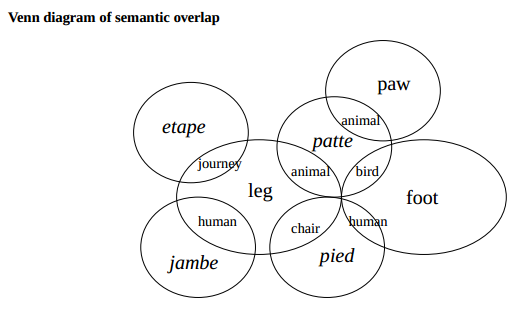
\includegraphics[width=12cm]{hutchins-leg-etc.png}
  \caption{Overlap of words related to ``leg"; relationships between English
  and French words. Translation is pretty complicated.}
  \label{fig:leg}
\end{figure}


%% XXX: this sentence needs some help
We will develop and extend at least two broad approaches for CL-WSD: the use
of multilingual evidence where available and sequence labeling.

Both of these techniques have been prototyped and presented at workshops, but
they will be refined significantly and integrated into a more general tool for
use in practice with MT systems.

\subsection{Using multilingual evidence}
For many languages, we have multiple bitext corpora, where each corpus covers a
different language pair. There are, for example, many bitext corpora available
for English and other languages, or for Spanish and other languages.
We would like to be able to make use of evidence from all of these corpora when
translating into any particular target language, if possible.
Each corpus may contain useful examples of a given source-language word,
and senses of that word may be lexicalized in varying, non-overlapping ways in
the different target languages.
We would want a CL-WSD system to be able to pick up on the relationships
between senses of a given word -- two target languages may happen to surface
the same sense distinctions, perhaps due to being related languages, or simply
by coincidence. Alternatively, a combination of translations into several
languages may provide evidence for a certain lexical choice in the target
language.

We could also imagine using a sense-annotated corpus to train a ``monolingual"
WSD system, and use this as a 
... basically ensemble methods for WSD.

This approach is informed by the work of Lefever and Hoste
\cite{lefever-hoste-decock:2011:ACL-HLT2011}, although their technique requires
an entire machine translation system to perform CL-WSD, which is somewhat
unwieldy when we want to use CL-WSD as a subcomponent of a machine translation
system.

Earlier this year, we developed a prototype CL-WSD system that makes use of
multilingual evidence \cite{rudnick-liu-gasser:2013:SemEval-2013} and produced
some of the best results in a SemEval shared task on CL-WSD \cite{task10}.
The task was to translate polysemous nouns from English into other European
languages. In our SemEval paper, we presented three variations on the approach:
a straightforward classification approach (without multilingual evidence), a
classifier stacking approach, and a graphical model system based on loopy
belief propagation over Markov networks.

The simplest system presented in that work, based on a maximum entropy
classifier, simply extracted features from a window around the English noun to
be translated and used these to make a prediction. The same system could also
return a probability distribution over target-language words or phrases. This
simple system was used as a subcomponent in the two more sophisticated systems.

The classifier stacking approach used 
for each available bitext corpus, for each source-language word that we want to
model, we train a classifier to predict translations from the source language
into the other language of the bitext.
Then we can include the output of that classifier as a feature when training
our classifier for the desired target language.


In the graphical model approach, we treat the problem of 
... this also has the property of explicitly handling the uncertainty of each
of the component classifiers.

\subsection{Lexical selection as a sequence labeling problem}
We will also investigate the use of sequence-labeling models for lexical
selection.  The intuition behind the sequence-labeling approach is that machine
translation implies an ``all-words" WSD task, in that we need to choose a
translation for every word or phrase in the source sentence, and that the
sequence of translations chosen should make sense when taken together.

One promising formalism for this line of work is the Maximum Entropy Markov
Model \cite{icml00/mccallum}, which can be combined in a straightforward way
with the simpler Hidden Markov Model (HMM).
This combination allows for efficient inference and the ability to trade more
computational resources for richer modeling. More sophisticated sequence
models, such as Conditional Random Fields, may be useful in this task as well.

We also developed a prototype CL-WSD system based on sequence labeling and
applied it to both English-Spanish and Spanish-Guarani translation tasks; this
work was presented at the HyTra workshop in August
\cite{rudnick-gasser:2013:HyTra-2013}.

For the sequence labeling approach in which only some words have their
translations modeled explicitly with a classifier, we have yet to explore what
the best approaches are for choosing \emph{which} words should get classifiers.

We will also look into the best ways to integrate the multilingual approach
with this one.

TODO look at the papers Nathan sent and be able to explain what other people
are doing for hard sequence labeling problems. That might go in the related
work section, or perhaps here.

\subsection{CL-WSD system combination}

Think about and expand the conversation I had with Markus.

You could imagine different CL-WSD systems rating each option separately and
then using MERT to get like an ensemble.
The question we were trying to address is like:
what if your n-gram model over labels for your source language has one idea
(this is the next likely label), and your emission probabilities say something
else (this is the label most likely to generate the observed input word)...
well, we could imagine just making several different decisions and letting the
decoder sort it out. We're doing that already actually, by including
phrase-table probabilities and a language model.
Are we just converging on the idea of a log-linear model again?
But the point here is that we don't have to have just one CL-WSD system. We can
have a bunch and let them fight it out. Hopefully this will help!

\subsection{Applying similar techniques for morphology prediction}

Sequence labeling has also been applied to the problem of generating
morphological features in target language text, so that target language output
words are appropriately inflected...
\cite{toutanova-suzuki-ruopp:2008:ACLMain}

This will be one of the approaches we investigate in the development of
Tereré...


%% \section{CL-WSD for Hybrid Machine Translation in Low-Resource Settings}
In recent years, we have seen renewed interest in machine translation systems
that take into account syntactic structure, linguistic knowledge, and semantic
representations.
Hopefully, these will provide better translation for language pairs with
significant reordering or syntactic divergences, and where one or both of the
languages has rich morphology.
The boundaries between rule-based and statistical MT systems are becoming
increasingly blurred, and hybrid systems are being developed in both
directions, with RBMT systems incorporating components based on machine
learning, as well as SMT systems making use of linguistic knowledge for
morphology and syntax.
Additionally, for most of the world's language pairs, there is simply no large
bitext corpus available, so training a purely statistical machine translation
system is infeasible.
Thus, while SMT approaches have had great success, and drastically changed the
machine translation landscape since the 1990s, RBMT approaches are still
relevant for many language pairs.

We would like for RBMT or hybrid systems, once developed, to be able to make
use of any bitext on hand.  Like SMT systems, they should be able to produce
better translations as larger corpora become available, without additional code
changes.

In this dissertation work, we will apply the CL-WSD techniques we develop to a
number of different MT systems with different designs, translating several
different language pairs.  These will include, at least: a hybrid SCFG-based
system that makes use of both bilingual transfer rules and a monolingual
language model, translating from Spanish to Guarani (Tereré) and a classic
transfer-based system translating Spanish to Quechua (Squoia).
We would also like to integrate into a more sophisticated RBMT system based on
constraint solving and synchronous dependency grammars (L3),
and a second system based on shallow transfer (Apertium), which has been
applied to a large number of language pairs.

\subsection{Tereré}
Since we hope that our ideas about lexical selection will make sense in several
different contexts, we will develop a new machine translation system out of
open-source SMT components, particularly relying on the cdec decoder and its
associated tools \cite{Dyer_etal_2010}.

This new system is called ``Tereré"
\footnote{\url{http://github.com/alexrudnick/terere}; 
Tereré is a cold variety of yerba mate brewed with ice water; it is a
specifically Paraguayan specialty.}.
Tereré will make use of modern hybrid MT techniques; our current design is
fairly similar to the Stat-XFER approach \cite{DBLP:conf/cicling/Lavie08}
developed by researchers at CMU.
Like Stat-XFER, Tereré will make use of bilingual transfer rules, a lexical
transfer stage, a target-language LM, and statistical decoding.

While the initial transfer rules will likely be written by hand, based the
respective grammars of Spanish and Guarani, we may also include
automatically-extracted rules, perhaps via Thrax \cite{weese-EtAl:2011:WMT} or
a forthcoming tool for extracting Inversion Transduction Grammars, from Dekai
Wu's team at HKUST \cite{saers-addanki-wu:2013:HyTra}.
The use of automatically-extracted transfer rules would make the system more
similar to the SAMT approaches of Zollmann and Venugopal
\shortcite{zollmann-venugopal:2006:WMT}.

In order to integrate our CL-WSD systems into Tereré, we will automatically
produce a SCFG rules just before decoding, in which features that encodes the
preferences of the WSD system are added to each lexical transfer rule. Then
the weights for all of the features provided to the system (translation
probabilities, LM scores, CL-WSD scores, and perhaps others) can be tuned with
MERT \cite{och:2003:ACL}, and the decoder will use these to search the space of
licensed translations.

We will approach the rich morphology of Guarani and the associated data
sparsity by having the system produce uninflected Guarani stems, which we will
then inflect in a second pass.
In the second pass, we will predict the appropriate morphological features will
with a discriminative sequence-labeling approach based on work at Microsoft
Research \cite{toutanova-suzuki-ruopp:2008:ACLMain}.
Thus both the transfer rules and the language model will be in terms of stemmed
Guarani.
As an alternative, we could adapt the techniques in
\cite{chahuneau:2013:emnlp} to generate translation rules that contain the
appropriately inflected target forms, just before running the decoder.
Rule-based approaches may also be sensible for generating Guarani morphology,
in some cases, and these will have to be investigated. In any case, once the
appropriate morphological features have been predicted, surface forms of
Guarani words will be generated with the FST-based morphological analyzer and
generator developed by Michael Gasser and described in
\cite{rudnick-gasser:2013:HyTra-2013}.

\subsection{SQUOIA}
SQUOIA\footnote{Described in detail at
\url{http://www.cl.uzh.ch/research/maschinelleuebersetzung/hybridmt_en.html}; 
Code available at \url{http://code.google.com/p/squoia/}}
is a project for MT from Spanish to Quechua, another relatively large
indigenous American language. SQUOIA is being developed by a team at the
University of Zurich. For the most part, it is a classical rule-based transfer
system, although the team has recently developed techniques for predicting verb
morphology with machine learning methods, in cases when rules cannot reliably
disambiguate \cite{riosgonzales-gohring:2013:HyTra}. It does not currently use
machine learning for lexical selection, although we have been in contact with
the team and are planning to collaborate to add CL-WSD features.

SQUOIA's architecture is based on the Matxin system \cite{matxin_2005}, which
was originally intended for translating from Spanish to Basque.
It consists of a pipeline of scripts, each of which passes along a tree
describing the current input sentence, in XML form. Adding CL-WSD to this
system will involve adding another script somewhere in the pipeline that
extracts features from the current annotated sentence, makes lexical choices,
and then passes these choices to subsequent scripts.

\subsection{L3}
L3 is an RBMT system based on synchronous dependency grammars and constraint
solving \cite{gasser:sxdg,gasser:aflat2012}.  It makes use of syntactic
knowledge about the source and target languages and can also include abstract
semantic representations as an intermediate stage in processing. Notably, L3
does not use a pipeline architecture: all of the constraints about the source
syntax, target syntax, semantic representation, and their relationships are
instantiated in one step, then solved jointly. L3 integrates morphological
analysis and generation for use in translating morphologically rich languages,
such as Guarani and Ethiopian semitic languages;
the morphological analyzers and generators to be used in Tereré were originally
developed for L3.

However, the constraints in L3 are currently unweighted, and it could use a way
to rank the licensed translations of an input sentence. It faces syntactic and
lexical ambiguity both in its analysis of the input sentence and in the
construction of output sentences. Ideally, a good lexical selection module
would constrain its other choices, yielding the higher-quality translations
first.

\subsection{Apertium}
Apertium\footnote{\url{http://www.apertium.org/}} \cite{Forcada_theapertium} is
another transfer-based RBMT system, originally designed for translating between
the languages of Spain but now handling over thirty language pairs. Some
language pairs are quite mature, while others are in prototype stages.

Apertium is a ``shallow transfer" system, meaning that it does not depend on
complete syntactic analysis of input sentences, but typically works by
chunking.
In his dissertation work (\cite{tyers-fst,tyers-thesis}), Francis Tyers has
been developing a new lexical selection system for Apertium, one that learns
lexical selection rules in the form of finite-state transducers from available
bitext. These rules are also human readable and editable, which seems like a
useful feature so that users can debug and tweak a translation system as
desired.
Tyers' lexical selection system is a strong baseline against which we should
compare our new CL-WSD approaches, and time and ingenuity permitting, we would
also like to integrate our system into Apertium.

%% \urldef{\leydelenguas}\url{http://www.cultura.gov.py/lang/es-es/2011/05/ley-de-lenguas-n%C2%BA-4251/}

\chapter{Paraguay and the Guarani Language}
Guarani is an indigenous language spoken in Paraguay and the surrounding
region.
Historically, it was the native language of the indigenous Guarani people. The
word for the Guarani language in Guarani is \emph{avañe'e} (``people's
language", where \emph{ñe'e} means ``language").

Guarani is unique among indigenous American languages in that a substantial
number of non-indigenous people speak it.  The majority of Paraguayans are
conversant in Guarani, although they are likely to be bilingual with Spanish.
In practice, many Paraguayans use a combination of Guarani and Spanish called
\emph{Jopar{\'a}}, which is the Guarani word for ``mixture".

Paraguay is officially a bilingual, pluricultural country, as described by its
famous \emph{Ley de Lenguas} \footnote{\leydelenguas} (``Law of Languages").
However, the Guarani language is at a significant social and economic
disadvantage and is typically not used in formal situations, as Spanish is
often considered more prestigious. There are, however, an engaged activist
community, many Guarani-language educators, and a government agency devoted
specifically to policy regarding language.
The Guarani language figures significantly into a sense of Paraguayan national
identity and history.

Guarani has a rich, polysynthetic, agglutinative morphology, in which roots can
derive into different parts of speech, and often several roots can combine into
a single word. Guarani morphology can mark tense, aspect (even on nouns),
number, negation, and other features. However, unlike Spanish, it has no
grammatical gender.  Guarani's rich morphology can make many NLP tasks,
including ones seemingly as simple as spell-checking, rather challenging.

We are in contact with a number of collaborators in Paraguay, including
language activists and educators from the \emph{Ateneo de la Lengua y Cultura
Guaraní} \footnote{\url{http://www.ateneoguarani.edu.py/}} and the
\emph{Fundación Yvy Marãe'{\~y}} \footnote{\url{http://yvymaraey.org/}},
both of which are schools that offer training for Guarani-language translators.

We have also started discussing development plans with several local software
developers -- including some from the local One Laptop Per Child organization
-- interested in building open source software, such as the corpus-building
websites described in the next section.

%% \section{Acquiring larger bitext corpora}
As part of the ongoing work for the practical goal of building a useful
Spanish-Guarani MT system, we would like to build larger training corpora,
containing both bitext and monolingual Guarani text.
To help in the collection, we plan to build two websites:
a collaborative online space for building translations of documents, 
and a searchable repository of Guarani and bilingual documents.
Initial designs for both of these sites were done as a master's project in HCI
by Alberto Samaniego\footnote{\url{http://albsama.com}}, who will hopefully
continue collaborating on this project from his native Paraguay.
We have also had helpful software contributions from
Rodrigo Villalba Zayas\footnote{\url{https://github.com/rodrigovz}} --
also from Paraguay -- and more potential collaborators have expressed
interest in helping, from Paraguay, Indiana, and the broader open-source world.

\subsection{Collecting Guarani Documents}
The first website we will develop is called ``Tahekami", which means
\emph{let's search together} in Guarani.
Tahekami is a repository of Guarani and bilingual documents that will allow
searching, browsing documents by tag, and uploading new documents.

An initial version of this site is already well underway
\footnote{\url{http://github.com/hltdi/gn-documents}}.  We have a working
search engine based on the Whoosh library
\footnote{\url{https://bitbucket.org/mchaput/whoosh/wiki/Home}} and some sample
documents -- twelve masters theses from the \emph{Ateneo}. We will need to
develop policies for which documents are permissible for distribution through
this site and work on integrating morphological analysis into the search
engine. Currently, new documents must be approved by an administrator before
being added to the index.

\subsection{Collecting Translations}
The second website, tentatively called ``Guampa"
\footnote{A ``guampa", in Paraguay, is the cup from which one drinks yerba mate
or tereré. The term ``guampa" is also local to Paraguay; in other parts of
South America, the container itself is called a ``mate".},
will be used by Guarani speakers and learners to produce translations of
relevant documents from Spanish to Guarani or vice-versa.
It will be something like a bilingual wiki, although the interface will
encourage users to edit sentences individually.
The software will segment the sentences in the initial
source-language documents and allow users to contribute translations for each
source sentence in turn, while showing the complete document context.
As a result of this, not only will will we be able to collect bitext training
data, but we will also produce useful translations.

Initially, this site will be seeded with documents from the Spanish and Guarani
Wikipedias. Successful translations of the Spanish-language articles could be
fed back into the Guarani Wikipedia. Other documents will be added by
Guarani-language educators and perhaps also pulled from Tahekami. Translations
may be assigned as homework by Guarani-language teachers.

The website will keep track of translations contributed by individual users;
there may be game-like features and community voting, where large number of
translations, or particularly good ones, are recognized, perhaps with virtual
prizes and badges.
Ideally, community management will be addressed by Paraguayan volunteers and
the gamification features can be built by contributors from the open source
world; this website and its richer features are not the primary focus of this
dissertation.

We may eventually collect enough bitext with this website such that it makes
sense to develop approaches for determining which sentences are the most
reliable and the most useful for training; this may correlate with quality
judgements from the human volunteers.
Investigating this relationship would make a good research question.

In the medium-term, this website will get an integrated ability to search
a translation memory and automatic suggestions from a machine translation
system\footnote{Features described in a presentation in Spanish here:
\url{http://www.cs.indiana.edu/~gasser/Taller2013/} ; English-language similar
presentation: \url{http://tinyurl.com/alexr-clingding-guarani} }
. While these features will be both useful and present a number of
interesting research questions, they are outside the scope of this
dissertation.

%% \section{Related Work}
\label{sec:relatedwork}

\subsection{Cross-lingual Word Sense Disambiguation}

While most SMT systems do not make use of an explicit WSD module, recently
Carpuat and Wu have shown how to use word-sense disambiguation techniques to
improve modern phrase-based SMT systems, in a normally 

\cite{carpuatpsd,carpuat-wu:2007:EMNLP-CoNLL2007,carpuat2008evaluation}


ParaSense, the system of Lefever
and Hoste, takes into account evidence from all of the available parallel
corpora. Let $S$ be the set of five target languages and $t$ be the particular
target language of interest at the moment; ParaSense creates bag-of-words
features from the translations of the target sentence into the languages $S -
\lbrace{t \rbrace}$.
Given corpora that are parallel over many languages, this is straightforward at
training time. However, at testing time it requires a complete MT system for
each of the four other languages, which is computationally prohibitive. Thus in
our work, we learn from several parallel corpora but require neither a locally
running MT system nor access to an online translation API.

Following the work of Lefever and Hoste
\shortcite{lefever-hoste-decock:2011:ACL-HLT2011}, we wanted to make use of
multiple bitext corpora for the CL-WSD task.

To our knowledge, there has not been other work on framing all-words WSD as a
sequence labeling problem. However, in monolingual WSD, Molina \textit{et al.}
\shortcite{DBLP:conf/iberamia/MolinaPS02}
have made use of HMMs for WSD. 


\subsection{Translation into Morphologically Rich Languages}



Chris Dyer's recent paper at EMNLP
\cite{chahuneau:2013:emnlp}

Talk about prediction for morphology.
\cite{toutanova-suzuki-ruopp:2008:ACLMain}

Also factored models...
\cite{yeniterzi-oflazer:2010:ACL}

\subsection{Hybrid Machine Translation for Under-Resourced Languages}
HMT for low-resource languages...

%% text from the HyTra paper
However, there has been work recently on using WSD techniques for translation
into lower-resourced languages, such as the English-Slovene language pair, as
in \cite{vintar-fivser-vrvsvcaj:2012:ESIRMT-HyTra2012}. 

The Apertium team has a particular practical interest in improving lexical
selection in RBMT; they recently have been developing
a new system, described in \cite{tyers-fst}, that learns finite-state
transducers for lexical selection from the available parallel corpora. It is
intended to be both very fast, for use in practical translation systems, and
to produce lexical selection rules that are understandable and modifiable by
humans.

Put in some stuff about SAMT and Stat-XFER.

Who's doing transfer rules that are hand-written?


\subsection{Creating Corpora Through Crowdsourcing}
There has been some work on creating multilingual corpora through
crowdsourcing, in several variations. Some projects have explicitly had the
goal of creating sentence-aligned bitexts useful for training MT systems, while
others have aimed to create useful resources for humans. Also the means of
crowdsourcing has varied; some contributors have been paid, and others are
volunteers.

Vamshi Ambati's recent work \cite{ambati_naacl,ambati_act} focuses on using
crowdsourcing and active learning to produce a corpus for English-Spanish SMT.
His system has a representation of which words and phrases it should learn
about, finding n-grams that are common in a development set but have little
support in the training set, and then automatically creates Mechanical Turk
tasks to elicit translations containing translations of these n-grams. This
work makes use of the relatively large population of Internet users (and thus
MTurk users) familiar with both English and Spanish, and succeeded in building
a large bitext corpus quickly and cheaply.

The Joshua team at Johns Hopkins has also successfully used Mechanical Turk to
crowdsource the creation of corpora for SMT
\cite{post-callisonburch-osborne:2012:WMT}. In this work, the team built
large parallel corpora for many languages of the Indian
subcontinent\footnote{\url{http://joshua-decoder.org/indian-parallel-corpora/}}
and developed a simple approach for discovering the high-quality contributions,
in which MTurk users vote on which translations they consider the best.

There's also MonoTrans
\url{http://www.cs.umd.edu/hcil/monotrans/}
"... an iterative protocol in which monolingual human participants work
together to improve imperfect machine translations." 

Contrastingly, the Tatoeba project is a repository of 
%% Tatoeba
Tatoeba -- repository of a bunch of example sentences translated into a variety
of languages.
\url{http://tatoeba.org/}

%% Tradubi
Tradubi project
\url{http://wiki.apertium.org/wiki/Tradubi}

(project seems to have died, though)

%% Traduwiki
Traduwiki
\url{http://traduwiki.org}

This looks awesome. If we could just bring up an instance of this, that would
be close to the right thing.

%% OPUS
OPUS, "the open parallel corpus".
\url{http://opus.lingfil.uu.se/}

\subsection{Online Language Tools for Guarani}

While there are not currently many online language tools for the Guarani, there
are a few ...

Notably, there is 
iGuarani
\url{http://iguarani.com/}

Wolf Lustig's dictionary
\footnote{\url{http://www.uni-mainz.de/cgi-bin/guarani2/dictionary.pl}}, which
has versions in Spanish, German, and English.


\footnote{\url{http://cafehistoria.ning.com/profiles/blogs/la-lengua-guarani-o-avanee-en}}

%% \section{Status and Expected Contributions}

Thus far, we have prototyped our CL-WSD systems that make use of multilingual
evidence and sequence labeling techniques and seen promising initial results
with these approaches, as described in \S\ref{sec:clwsd} and our papers
mentioned in that section.

Initial experiments are underway with building Tereré on top of the cdec
toolkit; we can already train Guarani-language LMs with KenLM
\cite{Heafield-estimate}, trained on the Guarani-language Wikipedia.
Additionally, we have mocked up the inclusion of CL-WSD features into the
decoder and started experimenting with writing SCFG transfer rules.

The Tahekami website is already well underway, and we have a web server on
which we can run Tahekami and Guampa. Fairly enthusiastic volunteers, including
developers from Paraguay, will likely continue helping in their development.

As a result of this work, we will have developed some new approaches for
CL-WSD and for building translation systems that target lower-resourced
languages. In this setting, phrase-based SMT is not feasible, so we have to
make effective use of our resources for the source language.
Practically, we should also have a new MT system for the Spanish-Guarani
language pair where there was previously none, an open-source reusable
package for helping RBMT systems make appropriate lexical choices, and a freely
available bitext corpus for a resource-poor language.


\bibliographystyle{is-abbrv}
\bibliography{dissertation}

\printindex

\end{document}
